% Chapter 4.  Four experiments, each with a simulation slot and a real-robot
% slot: eight slots.  Every slot follows one order: status; objective; process;
% dataset; results and analysis; summary; future plan.  Since 6 November 2026
% the slots of Experiments 1-3 are lifted from the raw write-ups under
% docs/report/insights/experiment_N/ (transformed by heading level only; edit
% the write-up, then regenerate); Experiment 4 still carries a verbatim
% fragment of the retired minor report for the tiny map.  An empty slot carries
% its status, the reason and the next action, and nothing else -- it never
% borrows the other domain's numbers.
\chapter[EXPERIMENTS AND RESULTS]{Experiments and Results}
\label{chap:results}

\textbf{Reporting cutoff:} 7 November 2026. On 6 November the dataset set was
fixed to the realistic-warehouse family in simulation
(\repo{dataset_allsensor_realistic_000}--\repo{003}, the two mapping
recordings and \repo{dataset_map_tiny}) and to \repo{dataset_realv6_000} and
\repo{dataset_realv7_000}--\repo{002} on the real robot; every result drawn
from any other recording was retired and is not reported.
\Cref{tab:slot-status} gives the status of the eight result slots. All four
simulation slots hold data; two real-robot slots hold provisional data and
two are planned, for the reason stated in each. Each
filled slot reports what was measured and its validity limits. Passages whose
evidence is not yet trustworthy, and the status note of each slot, are
collected in the separate Open Concerns document
(\repo{docs/report/concerns/concerns.pdf}), generated from this chapter's
source.

\begin{table}[htbp]
\centering
\caption{Status of the eight result slots at the reporting cutoff.}
\label{tab:slot-status}
\small
\begin{tabularx}{\textwidth}{>{\raggedright\arraybackslash}p{0.30\textwidth}>{\raggedright\arraybackslash}X>{\raggedright\arraybackslash}X}
\toprule
Experiment & Simulation & Real robot \\
\midrule
1. Estimator comparison against a non-visual baseline & \status{completed}:
  four realistic recordings, two layouts, with and without traffic; the
  non-visual estimators and twenty visual runs, one per cell; the loop closer
  decides ORB-SLAM3's error; latency and resources from eighteen repeats on
  the two mapping recordings & \status{partial}: wheel+gyro dead reckoning
  with a fitted speed scale and sixteen ORB-SLAM3 runs on four tracker-truthed
  recordings, the two families in the same accuracy class; VINS-Fusion has no
  valid run; no EKF (no steering measurement) \\
2. Offline YOLO detector performance & \status{completed}: four realistic
  recordings, 12\,698 frames, four-class checkpoint; precision 0.75,
  moving-object recall 0.29 & \status{planned}: no annotated frames \\
3. Dense map reconstruction and map quality & \status{partial}: tiny map
  passes; four realistic maps fail the criterion; large map \status{failed};
  no map built with traffic present & \status{planned} \\
4. Autonomous navigation on the reconstructed map & \status{partial}: seven
  live runs in three of the four worlds track ground truth to a median of
  \SI{0.50}{\metre} over hand-driven routes, one losing the pose; no goal was
  commanded, so the goal-reaching half remains \status{planned} &
  \status{planned} \\
\bottomrule
\end{tabularx}
\end{table}

% =====================================================================
\FloatBarrier
\section{Experiment 1: Estimator Comparison Against a Non-Visual Baseline}
\label{sec:exp1}

\FloatBarrier
\subsection{Simulation}
\label{sec:results-proprio}
\label{sec:results-validity}
\label{sec:realistic-ab}
\label{sec:rpe}
\label{sec:trajectory-results}
\label{sec:exp1-sim}

\slotstatus{completed}{Four \repo{dataset_allsensor_realistic} recordings, two
layouts each recorded without and with warehouse traffic. Two families of
estimator are scored over the full common interval of each: the non-visual
ones --- wheel odometry, IMU dead reckoning, an EKF at the visual systems' own
inertial noise configuration and a measured-noise EKF as diagnostic --- and
the visual ones, VINS-Fusion once per recording and ORB-SLAM3 with a CPU or
GPU feature extractor and its loop closer active or disabled. Traffic is noted
as a condition, not tested as a factor. The latency and resource measurement
is taken from eighteen repeated runs on the two mapping recordings, three
repeats of each of six configurations, and those repeats are the only
within-configuration spread the campaign measures.}

\textbf{Objective.} Establish how well each estimator localises the robot on
the realistic warehouse, whether a non-visual estimator is competitive with the
visual pipelines on the same recordings, which of a visual pipeline's own
switches decides its error, and at what compute cost. A secondary question is
whether each estimator's reported uncertainty describes its error.

\textbf{Process.} Two groups of runs share these recordings.

\emph{Non-visual.} \repo{script/proprio_estimator.py calibrate} measured
each recording's wheel and inertial biases and wheel noise against ground truth
from its stationary head and its driven length; \repo{run} produced the wheel,
IMU and EKF trajectories offline; \repo{script/analyse_proprio.py} scored them
with the live VINS-Fusion and ORB-SLAM3 runs over the common interval. The
EKF reported here does \emph{not} use the measured inertial noise: by the
design decision of 6 November 2026 its three inertial noise terms are the
values both visual configurations declare (\repo{config/wil_sim/stereo_imu.yaml}:
gyroscope density \num{0.002}, accelerometer density \num{0.02}, gyroscope bias
walk \num{1e-4}), converted to per-sample $\sigma$ at \SI{200}{\hertz} by
\repo{script/make_vslam_noise_yaml.py}, so that the proprioceptive and visual
families run on the same hand-set inertial model; biases and both wheel
$\sigma$ have no visual counterpart and stay measured. The measured-noise
filter is run beside it as a diagnostic row and is not the baseline.

\emph{Visual.} Every run replayed at rate 1.0 from the bag with the
node live on the laptop, the deployment condition; no detector ran. VINS-Fusion
ran once per recording (run \repo{cpu}). ORB-SLAM3 ran four times per
recording: the CPU or the GPU feature extractor (fork patches 10/10b, runs
\repo{*_cpu} and \repo{*_gpu}), each with the loop closer active
(\repo{loopclosing_*}) or disabled (\repo{noloopclosing_*}), all on 6 November
2026 with the same node binary and configuration
(\repo{config/wil_sim/stereo_imu.yaml}). One run per cell, so no
within-condition spread exists.

\textbf{Datasets.} \Cref{tab:exp1-datasets}: the two static twins and the
two traffic recordings of the realistic worlds, both layouts. Traffic is noted
as a condition of a recording, not treated as a factor, since no two
recordings share a route.

\begin{table}[htbp]
\centering
\caption[Recordings of Experiment 1.]{Recordings of Experiment~1 (names without the
\repo{dataset_allsensor_} prefix), from the bags. Route is the ground-truth
path length; samples are ground-truth odometry messages.}
\label{tab:exp1-datasets}
\small
\begin{tabular}{lllrrr}
\toprule
Recording & Layout & Traffic & Route [\si{\metre}] & Span [\si{\second}] & Samples \\
\midrule
\repo{realistic_000} & U & none (static twin) & 171.3 & 125.5 & 6\,278 \\
\repo{realistic_001} & I & none (static twin) & 133.0 & 96.9 & 4\,847 \\
\repo{realistic_002} & U & pallet jacks and people & 102.7 & 79.5 & 3\,975 \\
\repo{realistic_003} & I & pallet jacks and people & 158.0 & 117.0 & 5\,852 \\
\bottomrule
\end{tabular}
\end{table}

\emph{Which recording is which.} \repo{realistic_000} (U layout) and \repo{_001} (I
layout) are the static twins; \repo{_002} (U) and \repo{_003} (I) carry ten and
twelve moving props, pallet jacks on pick--carry--drop jobs and walking people.
Routes are 103 to \SI{171}{\metre} over 80 to \SI{126}{\second}
(\cref{tab:exp1-datasets}); no two recordings share a
route.

\textbf{Reporting rules.} Aligned ATE is RMSE after a rigid $SE(3)$ fit
with scale fixed, the convention of every slot; anchored error is the direct
difference from ground truth with no alignment and is defined only for the
estimators that start from the ground-truth pose; aligned rotation is the
geodesic angle after the same fit, defined for every estimator; ANEES is the
average normalised estimation error squared over decorrelated \SI{1}{\hertz}
samples, 3.0 for a consistent planar filter. Ground truth is the bag's
\repo{/ground_truth/odometry} moved from the model origin to the IMU point
every estimator reports (lever arm \SI{0.338}{\metre} forward,
\SI{0.192}{\metre} up). The visual runs are pinned by name: VINS-Fusion
\repo{cpu}; ORB-SLAM3 \repo{loopclosing_gpu} and \repo{noloopclosing_gpu},
both with the GPU feature extractor, at replay rate 1.0. The loop-closer
state is read from each run's \repo{loop_closing.csv} (patch-7 signature:
sub-millisecond rows mean a disabled closer), not from the run name. On
\repo{realistic_002} the directory named \repo{loopclosing_gpu} first held a
run whose manifest names the \repo{realistic_003} bag (3\,535 stereo pairs
received against the 2\,409 that recording holds); it was scored against the
wrong truth for a day, is set aside under
\repo{trash/output/misfiled_20261106/}, and the run reported here was made on
the right bag on the evening of 6 November (2\,382 pairs received). Sources: \path{output/compare/simulation/exp1-realistic/}
(\repo{proprio_metrics.csv}, \repo{proprio_rpe_metrics.csv}, the noise models
under \repo{noise/}), run directories under \path{output/output_{wheel,imu,ekf,ekf_measured}/simulation/}. One run per cell, $n=1$.

\paragraph{Reporting rules, visual arms.}
Every run is reported on its own. Aligned ATE is RMSE after a rigid $SE(3)$
fit with scale fixed, in three dimensions; RPE at \SI{1}{\second} is
translational over pairs that span no jump (a step above
\SI{10}{\metre\per\second} between consecutive poses). The loop-closer state
is read from \repo{loop_closing.csv} (sub-millisecond rows mean a disabled
closer), not from the run name, and every closure the closer accepted is
listed with its time and correction. Ground truth is the bag's
\repo{/ground_truth/odometry}, moved from the model origin to the IMU point
both estimators report (lever arm \SI{0.338}{\metre} forward,
\SI{0.192}{\metre} up) before alignment; the figures draw that moved path.
``Kept'' is the fraction of the bag's stereo pairs the node processed, so
frames lost before the node's own counter count as lost. The onset analysis
uses the start-anchored planar error against a threshold of three times the
estimator's median error over its two static runs (VINS-Fusion
\SI{1.07}{\metre}, ORB-SLAM3 \SI{1.31}{\metre}). Sources: \path{output/compare/simulation/exp-realistic-ab/}
(\repo{runs_metrics.csv}, \repo{baseline_table.tex}),
\path{output/compare/simulation/exp3-timelines/}
(\repo{timelines.csv}, \repo{thresholds.csv}), run directories under
\path{output/output_orb/simulation/} and \path{output/output_vins/simulation/}.
The run that first occupied \path{realistic_002/loopclosing_gpu} had been
launched on the \repo{realistic_003} bag with the wrong output path (its
manifest names that bag and world, and it received 3\,535 stereo pairs where
\repo{realistic_002} holds 2\,409); it is set aside under
\path{trash/output/misfiled_20261106/} and the cell was re-run on the right
bag on the evening of 6 November.

\subsubsection{Non-visual estimators}

\paragraph{Results.} At the visual systems' inertial noise the EKF holds
\SIrange{0.68}{2.80}{\metre} aligned ATE and is behind VINS-Fusion on all four
recordings; the measured-noise diagnostic holds \SIrange{0.21}{0.58}{\metre}.
\Cref{tab:exp1-accuracy} gives every estimator on every recording,
\cref{tab:exp1-rpe} the relative pose error at \SI{1}{\second}, and
\cref{fig:exp1-grid} the trajectories.

\begin{table}[htbp]
\centering
\caption[Estimator comparison on the four realistic recordings.]{Estimator
comparison on the four realistic recordings. The closer state of each
ORB-SLAM3 run is read from its artefact. ANEES is reported for the
proprioceptive estimators, which carry a covariance; a consistent filter
gives 3.0, and every value here is above it. \textbf{Bold} marks the lowest aligned ATE of a recording; the measured-noise filter is a diagnostic row, not the baseline, so it is shown bold where it is lowest but is not the slot's result.}
\label{tab:exp1-accuracy}
\scriptsize
\setlength{\tabcolsep}{3pt}
\resizebox{\textwidth}{!}{%
\begin{tabular}{lllrrrrrr}
\toprule
Recording & Estimator & Closer & Anch.\ RMS & Anch.\ final & Aligned ATE & Aligned rot. & Yaw RMS & ANEES \\
 & & & [\si{\metre}] & [\si{\metre}] & [\si{\metre}] & [\si{\degree}] & [\si{\degree}] & \\
\midrule
\repo{realistic_000} & Wheel odometry & -- & 5.89 & 5.66 & 2.56 & 9.14 & 18.05 & 1810 \\
 & IMU dead reckoning & -- & 36.19 & 76.01 & 23.02 & 177.21 & 0.84 & 454 \\
 & EKF, VSLAM-config noise & -- & 2.49 & 3.42 & 1.34 & 5.83 & 10.62 & 19 \\
 & EKF, measured noise (diag.) & -- & 0.33 & 0.35 & \textbf{0.23} & 0.47 & 0.43 & 111 \\
 & VINS-Fusion & -- & -- & -- & 0.29 & 1.85 & -- & -- \\
 & ORB-SLAM3 GPU, LC run & active & -- & -- & 0.29 & 12.80 & -- & -- \\
 & ORB-SLAM3 GPU, no-LC run & disabled & -- & -- & 0.52 & 12.84 & -- & -- \\
\midrule
\repo{realistic_001} & Wheel odometry & -- & 1.40 & 2.90 & 1.03 & 6.04 & 7.27 & 176 \\
 & IMU dead reckoning & -- & 15.40 & 39.82 & 13.05 & 0.25 & 0.55 & 160 \\
 & EKF, VSLAM-config noise & -- & 0.94 & 0.83 & 0.68 & 3.81 & 4.51 & 8 \\
 & EKF, measured noise (diag.) & -- & 0.26 & 0.26 & \textbf{0.21} & 0.33 & 0.36 & 31 \\
 & VINS-Fusion & -- & -- & -- & 0.22 & 1.18 & -- & -- \\
 & ORB-SLAM3 GPU, LC run & active & -- & -- & 4.78 & 18.98 & -- & -- \\
 & ORB-SLAM3 GPU, no-LC run & disabled & -- & -- & 0.40 & 15.13 & -- & -- \\
\midrule
\repo{realistic_002} & Wheel odometry & -- & 6.54 & 6.08 & 4.81 & 17.03 & 25.00 & 1778 \\
 & IMU dead reckoning & -- & 25.88 & 39.17 & 19.01 & 118.74 & 1.91 & 695 \\
 & EKF, VSLAM-config noise & -- & 2.06 & 3.29 & 1.58 & 9.92 & 13.65 & 37 \\
 & EKF, measured noise (diag.) & -- & 0.59 & 0.30 & 0.37 & 0.70 & 1.03 & 191 \\
 & VINS-Fusion & -- & -- & -- & 0.66 & 3.57 & -- & -- \\
 & ORB-SLAM3 GPU, LC run & active & -- & -- & 0.40 & 16.04 & -- & -- \\
 & ORB-SLAM3 GPU, no-LC run & disabled & -- & -- & \textbf{0.17} & 16.08 & -- & -- \\
\midrule
\repo{realistic_003} & Wheel odometry & -- & 6.71 & 7.19 & 4.30 & 19.24 & 35.82 & 3399 \\
 & IMU dead reckoning & -- & 13.72 & 35.47 & 11.60 & 180.00 & 1.68 & 140 \\
 & EKF, VSLAM-config noise & -- & 4.44 & 6.23 & 2.80 & 15.92 & 28.01 & 158 \\
 & EKF, measured noise (diag.) & -- & 0.79 & 1.49 & 0.58 & 3.90 & 5.72 & 106 \\
 & VINS-Fusion & -- & -- & -- & \textbf{0.27} & 1.51 & -- & -- \\
 & ORB-SLAM3 GPU, LC run & active & -- & -- & 0.50 & 13.16 & -- & -- \\
 & ORB-SLAM3 GPU, no-LC run & disabled & -- & -- & 1.91 & 13.53 & -- & -- \\
\bottomrule
\end{tabular}}
\end{table}

\begin{table}[htbp]
\centering
\caption[Relative pose error at $\Delta t=\SI{1}{\second}$ on the four
realistic recordings.]{Relative pose error at $\Delta t=\SI{1}{\second}$, RMSE
over all pairs and over pairs that span no detected jump (a step above
\SI{10}{\metre\per\second} between consecutive poses); the jump count is per
run. \textbf{Bold} marks the lowest jump-free translational RPE of a recording.}
\label{tab:exp1-rpe}
\scriptsize
\setlength{\tabcolsep}{3pt}
\begin{tabular}{llrrrrr}
\toprule
Recording & Estimator & Jumps & \multicolumn{2}{c}{Translation [\si{\metre}]} & \multicolumn{2}{c}{Rotation [\si{\degree}]} \\
 & & & all pairs & clean & all pairs & clean \\
\midrule
\repo{realistic_000} & Wheel odometry & 0 & 0.028 & 0.028 & 1.720 & 1.720 \\
 & IMU dead reckoning & 0 & 1.941 & 1.941 & 0.023 & 0.023 \\
 & EKF & 44 & 0.240 & 0.218 & 0.979 & 0.893 \\
 & EKF & 0 & 0.039 & 0.039 & 0.098 & 0.098 \\
 & VINS-Fusion & 0 & 0.021 & 0.021 & 0.443 & 0.443 \\
 & ORB-SLAM3 GPU, LC run & 3 & 0.246 & 0.017 & 5.902 & 0.094 \\
 & ORB-SLAM3 GPU, no-LC run & 3 & 0.254 & \textbf{0.013} & 5.909 & 0.090 \\
\midrule
\repo{realistic_001} & Wheel odometry & 0 & 0.033 & 0.033 & 1.733 & 1.733 \\
 & IMU dead reckoning & 0 & 0.980 & 0.980 & 0.023 & 0.023 \\
 & EKF & 42 & 0.254 & 0.202 & 0.964 & 0.811 \\
 & EKF & 0 & 0.045 & 0.045 & 0.090 & 0.090 \\
 & VINS-Fusion & 0 & 0.018 & \textbf{0.018} & 0.366 & 0.366 \\
 & ORB-SLAM3 GPU, LC run & 7 & 1.191 & 0.034 & 7.031 & 0.120 \\
 & ORB-SLAM3 GPU, no-LC run & 2 & 0.302 & 0.020 & 6.845 & 0.155 \\
\midrule
\repo{realistic_002} & Wheel odometry & 0 & 0.027 & 0.027 & 1.997 & 1.997 \\
 & IMU dead reckoning & 0 & 1.505 & 1.505 & 0.033 & 0.033 \\
 & EKF & 67 & 0.243 & 0.158 & 0.985 & 0.780 \\
 & EKF & 0 & 0.035 & 0.035 & 0.075 & 0.075 \\
 & VINS-Fusion & 0 & 0.038 & 0.038 & 0.790 & 0.790 \\
 & ORB-SLAM3 GPU, LC run & 4 & 0.463 & \textbf{0.017} & 10.403 & 0.084 \\
 & ORB-SLAM3 GPU, no-LC run & 1 & 0.147 & 0.028 & 7.422 & 0.070 \\
\midrule
\repo{realistic_003} & Wheel odometry & 0 & 0.023 & 0.023 & 1.447 & 1.447 \\
 & IMU dead reckoning & 0 & 0.936 & 0.936 & 0.023 & 0.023 \\
 & EKF & 22 & 0.202 & 0.185 & 1.026 & 0.969 \\
 & EKF & 0 & 0.036 & 0.036 & 0.154 & 0.154 \\
 & VINS-Fusion & 0 & 0.014 & \textbf{0.014} & 0.327 & 0.327 \\
 & ORB-SLAM3 GPU, LC run & 3 & 0.165 & 0.028 & 6.068 & 0.174 \\
 & ORB-SLAM3 GPU, no-LC run & 3 & 0.151 & 0.036 & 6.088 & 0.333 \\
\bottomrule
\end{tabular}
\end{table}

\begin{figure}[p]
  \centering
  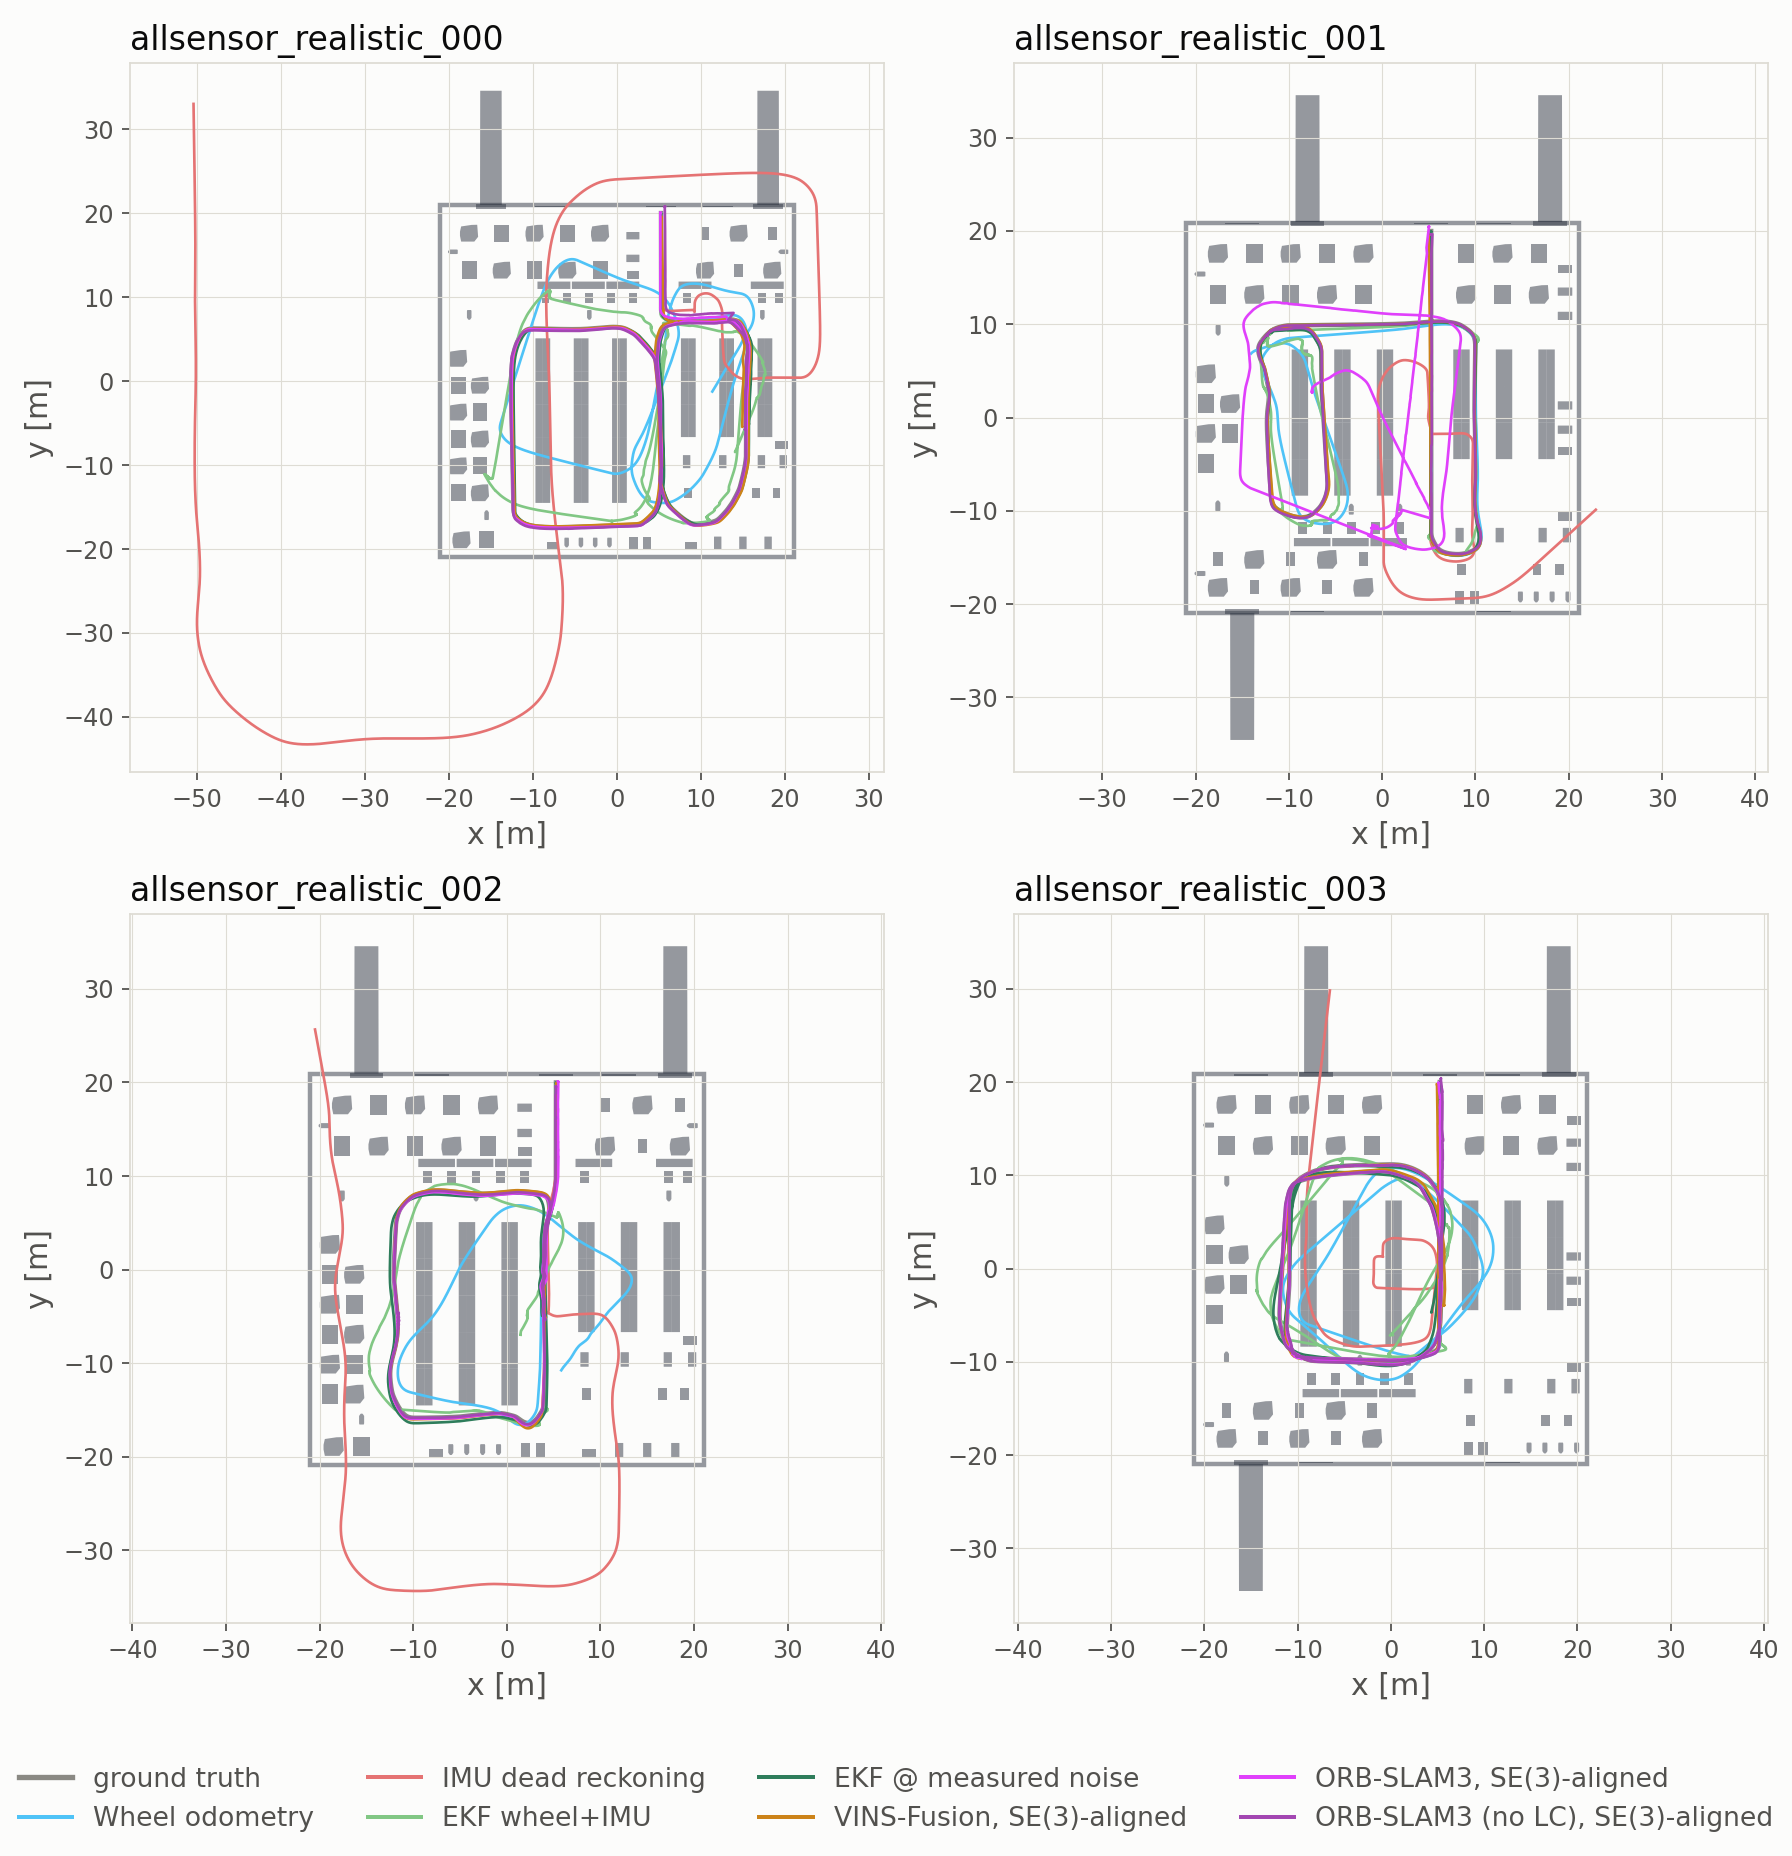
\includegraphics[width=0.96\textwidth]{figures/proprio_trajectories_grid_realistic.png}
  \caption[Estimator comparison on every realistic recording, world frame.]{
  Estimator comparison on every realistic recording, world frame: the
  dead-reckoning estimators as estimated from the ground-truth start pose,
  the visual estimators after the rigid $SE(3)$ alignment used for their
  metrics, one legend for all four panels. The IMU leaves the building on
  every recording; the EKF at the visual systems' noise (light green) wanders
  in heading where the measured-noise filter (dark green) stays on the route;
  ORB-SLAM3's divergent runs are the excursions on \repo{001} (loop closer
  active) and \repo{003} (closer disabled).}
  \label{fig:exp1-grid}
\end{figure}

\paragraph{Analysis.} With both families on the same hand-set inertial model
the ordering is settled: VINS-Fusion is the most accurate estimator on every
recording (\SIrange{0.22}{0.66}{\metre}) and the EKF, at
\SIrange{0.68}{2.80}{\metre}, is behind it on all four and behind the better
ORB-SLAM3 run on three. The measured-noise diagnostic puts the same filter at
\SIrange{0.21}{0.58}{\metre}, ahead of VINS-Fusion on three of four, so the
whole of the EKF's deficit is the noise model and none of it the
architecture --- the September control, reproduced on new recordings and
larger.

The mechanism is the one isolated in September. The configuration's
gyroscope density is five to seven times the measured value, which inflates
the heading process noise forty-fold; with the heading unobserved except
through the wheel yaw-rate residual, that residual steers the heading instead
of the bias, and yaw RMS rises from \SIrange{0.4}{5.7}{\degree} to
\SIrange{4.5}{28.0}{\degree}. On routes of 100 to \SI{170}{\metre} with
repeated turns that heading error is what the aligned ATE measures.

ORB-SLAM3's divergences are not a loop-closure effect. With the GPU front end
six of eight runs hold \SIrange{0.17}{0.52}{\metre} and two diverge, to
\SI{4.78}{\metre} with the closer active on \repo{realistic_001} and to
\SI{1.91}{\metre} with it disabled on \repo{realistic_003}, while the other
closer state on each of those recordings holds \SI{0.40}{} and
\SI{0.50}{\metre}. Each divergent run carries three or seven jumps
(\cref{tab:exp1-rpe}) and its clean relative error is as low as the stable
runs', so the error is a few discrete events, not steady-state tracking.
Which front-end condition produces them is not isolated here; the CPU runs of
the same recordings are scored below, where the same pattern recurs.

Traffic appears as a condition, not a tested factor. VINS-Fusion is
\SI{0.66}{\metre} on the U traffic recording against \SI{0.29}{\metre} on its
static twin and \SI{0.27}{\metre} against \SI{0.22}{\metre} on the I layout;
the proprioceptive estimators are unaffected by construction. The U recordings
do not share a route, so the difference cannot be credited to traffic alone.

The complementary failure of the two proprioceptive sensors holds. The IMU
keeps heading to \SIrange{0.5}{1.9}{\degree} RMS and loses position by
\SIrange{12}{23}{\metre}; the wheels keep position to \SIrange{1.0}{4.8}{\metre}
and lose \SIrange{7}{36}{\degree} of heading. Every proprioceptive covariance
is overconfident: ANEES \SIrange{8}{3399}{} against 3.0, the EKF at the
configuration noise least so because its inflated process noise is closer to
the error it actually makes.

\subsubsection{Visual estimators}

\paragraph{Results.} VINS-Fusion holds \SIrange{0.22}{0.66}{\metre} aligned
ATE on the four recordings with no jump and \SIrange{1.2}{3.6}{\degree} of
rotation error; its worst recording is the U layout with traffic,
\SI{0.66}{\metre} against \SI{0.29}{\metre} on that layout's static twin,
while on the I layout traffic changes nothing (\SI{0.27}{} against
\SI{0.22}{\metre}). ORB-SLAM3 spans \SIrange{0.14}{6.02}{\metre}: eleven of its
sixteen runs lie between \SI{0.14}{} and \SI{0.52}{\metre} and five diverge, and
which five is decided by the loop closer and the recording, not by the front
end (\cref{tab:realistic-baseline}, \cref{fig:realistic-traj,fig:realistic-metrics}).
Neither front end loses tracking on any recording, with or without traffic:
zero tracking-loss events and zero resets in twenty runs.

Two columns of \cref{tab:realistic-baseline} qualify those RMSE figures. The
first is the worst single error each run reaches after its initialisation
transient, which the RMSE averages away: over the fifteen runs that held it is
\SIrange{0.26}{1.25}{\metre}, between \num{0.8} and \num{2.6} times the run's
own RMSE, so no run that tracked was ever more than about
\SI{1.25}{\metre} from the truth; over the five that diverged it is
\SIrange{2.25}{13.42}{\metre}. The two orderings are not the same one. On
\repo{realistic_000} VINS-Fusion has the lower RMSE
(\SI{0.290}{} against \SI{0.338}{\metre}) and ORB-SLAM3 the smaller worst
case (\SI{0.260}{} against \SI{0.576}{\metre}), so which estimator is
``better'' on that recording depends on whether the question is average
accuracy or the largest excursion --- and for a vehicle in a \SI{3.0}{\metre}
aisle it is the second. The exclusion matters: every ORB-SLAM3 run peaks near
\SI{2.5}{\second} at three to four metres on the gravity re-alignment that
ends its inertial initialisation, and a raw maximum would report that
initialisation as though it were driving.

The second column is the same ATE as a percentage of the ground-truth path
length. It exists so that these \SIrange{103}{172}{\metre} routes can be set
beside the real robot's much shorter ones
(\cref{sec:sim-vs-real}), and it separates the two outcomes more sharply than
the metre figure does: \SIrange{0.09}{0.64}{\percent} for the fifteen runs
that held against \SIrange{1.11}{4.51}{\percent} for the five that diverged.
It is a ratio of two quantities already in the table, not a KITTI-style
sub-sequence drift rate, and it is not comparable to one.

% Generated by script/analyse_realistic_runs.py -- do not edit by hand.
\begin{table}[htbp]
\centering
\caption[Visual estimators on the four realistic-warehouse recordings.]{Visual estimators on the four realistic-warehouse recordings, 6 November 2026, replay rate 1.0. Aligned ATE is RMSE after a rigid $SE(3)$ fit with scale fixed; RPE is translational, at $\Delta=\SI{1}{\second}$ over pairs that do not span a jump; ``Jumps'' counts steps above \SI{10}{\metre\per\second}; ``Kept'' is the fraction of the bag's stereo pairs the estimator processed (frames lost before the node's own queue count as lost). Loop-closer state is read from \repo{loop_closing.csv}, not from the run name. Static and dynamic rows of one layout share a world geometry and differ in traffic only. ``Max'' is the largest single position error the run reaches \emph{after} its initialisation transient --- the same cut the onset analysis of \cref{tab:realistic-timelines-baseline} makes, after the last jump inside the first \SI{15}{\second} --- on the same alignment as the ATE column, and records the excursion that the RMSE averages away. Every ORB-SLAM3 run peaks near \SI{2.5}{\second} on the gravity re-alignment that ends its inertial initialisation, at three to four metres; that peak is excluded here because it measures the initialisation and not the driving. ``ATE/path'' is the aligned ATE as a percentage of the ground-truth path length, so that runs over routes of different length can be compared; it is a ratio, not a sub-sequence drift rate. \textbf{Bold} marks the lowest ATE, the lowest Max and the lowest jump-free RPE among the five arms of a recording; with one run per arm it records which run came lowest, not that the arm is better.}
\label{tab:realistic-baseline}
\small
\resizebox{\textwidth}{!}{%
\begin{tabular}{llll rrrrrrrr}
\toprule
Recording & Layout & Scene & Estimator & ATE [\si{\metre}] & Max [\si{\metre}] & ATE/path [\si{\percent}] & Rot.\ [\si{\degree}] & RPE$_{1\,\mathrm{s}}$ [\si{\metre}] & Jumps & Kept & Resets \\
\midrule
\repo{realistic_000} & U & static & ORB-SLAM3 & 0.338 & \textbf{0.260} & 0.20 & 13.74 & 0.083 & 2 & 0.72 & 0 \\
 &  &  & ORB-SLAM3 GPU & 0.293 & 0.525 & 0.17 & 12.80 & 0.079 & 3 & 0.99 & 0 \\
 &  &  & ORB-SLAM3 (no LC) & 0.483 & 1.249 & 0.28 & 14.05 & 0.090 & 2 & 0.74 & 0 \\
 &  &  & ORB-SLAM3 GPU (no LC) & 0.523 & 0.995 & 0.30 & 12.84 & \textbf{0.078} & 3 & 0.99 & 0 \\
 &  &  & VINS-Fusion & \textbf{0.290} & 0.576 & 0.17 & 1.85 & 0.084 & 0 & 0.77 & 0 \\
\addlinespace
\repo{realistic_001} & I & static & ORB-SLAM3 & 6.021 & 12.591 & 4.51 & 16.92 & 0.094 & 6 & 0.73 & 0 \\
 &  &  & ORB-SLAM3 GPU & 4.780 & 13.421 & 3.58 & 18.98 & 0.092 & 7 & 0.99 & 0 \\
 &  &  & ORB-SLAM3 (no LC) & 0.496 & 0.642 & 0.37 & 16.05 & 0.093 & 1 & 0.74 & 0 \\
 &  &  & ORB-SLAM3 GPU (no LC) & 0.400 & 0.514 & 0.30 & 15.13 & \textbf{0.088} & 2 & 0.97 & 0 \\
 &  &  & VINS-Fusion & \textbf{0.221} & \textbf{0.456} & 0.17 & 1.18 & 0.089 & 0 & 0.78 & 0 \\
\addlinespace
\repo{realistic_002} & U & dynamic & ORB-SLAM3 & 1.393 & 2.254 & 1.35 & 16.99 & \textbf{0.078} & 4 & 0.77 & 0 \\
 &  &  & ORB-SLAM3 GPU & 0.400 & 0.595 & 0.39 & 16.04 & \textbf{0.078} & 4 & 0.98 & 0 \\
 &  &  & ORB-SLAM3 (no LC) & 0.293 & 0.501 & 0.28 & 17.12 & 0.080 & 2 & 0.83 & 0 \\
 &  &  & ORB-SLAM3 GPU (no LC) & \textbf{0.170} & \textbf{0.255} & 0.16 & 16.08 & 0.083 & 1 & 0.99 & 0 \\
 &  &  & VINS-Fusion & 0.663 & 1.136 & 0.64 & 3.57 & 0.116 & 0 & 0.88 & 0 \\
\addlinespace
\repo{realistic_003} & I & dynamic & ORB-SLAM3 & \textbf{0.139} & \textbf{0.316} & 0.09 & 13.52 & 0.075 & 2 & 0.94 & 0 \\
 &  &  & ORB-SLAM3 GPU & 0.504 & 0.756 & 0.32 & 13.16 & 0.076 & 3 & 0.99 & 0 \\
 &  &  & ORB-SLAM3 (no LC) & 1.755 & 2.741 & 1.11 & 14.22 & 0.080 & 2 & 0.88 & 0 \\
 &  &  & ORB-SLAM3 GPU (no LC) & 1.911 & 2.800 & 1.21 & 13.53 & 0.083 & 3 & 0.99 & 0 \\
 &  &  & VINS-Fusion & 0.268 & 0.537 & 0.17 & 1.51 & \textbf{0.071} & 0 & 0.87 & 0 \\
\bottomrule
\end{tabular}}
\end{table}


\begin{figure}[p]
  \centering
  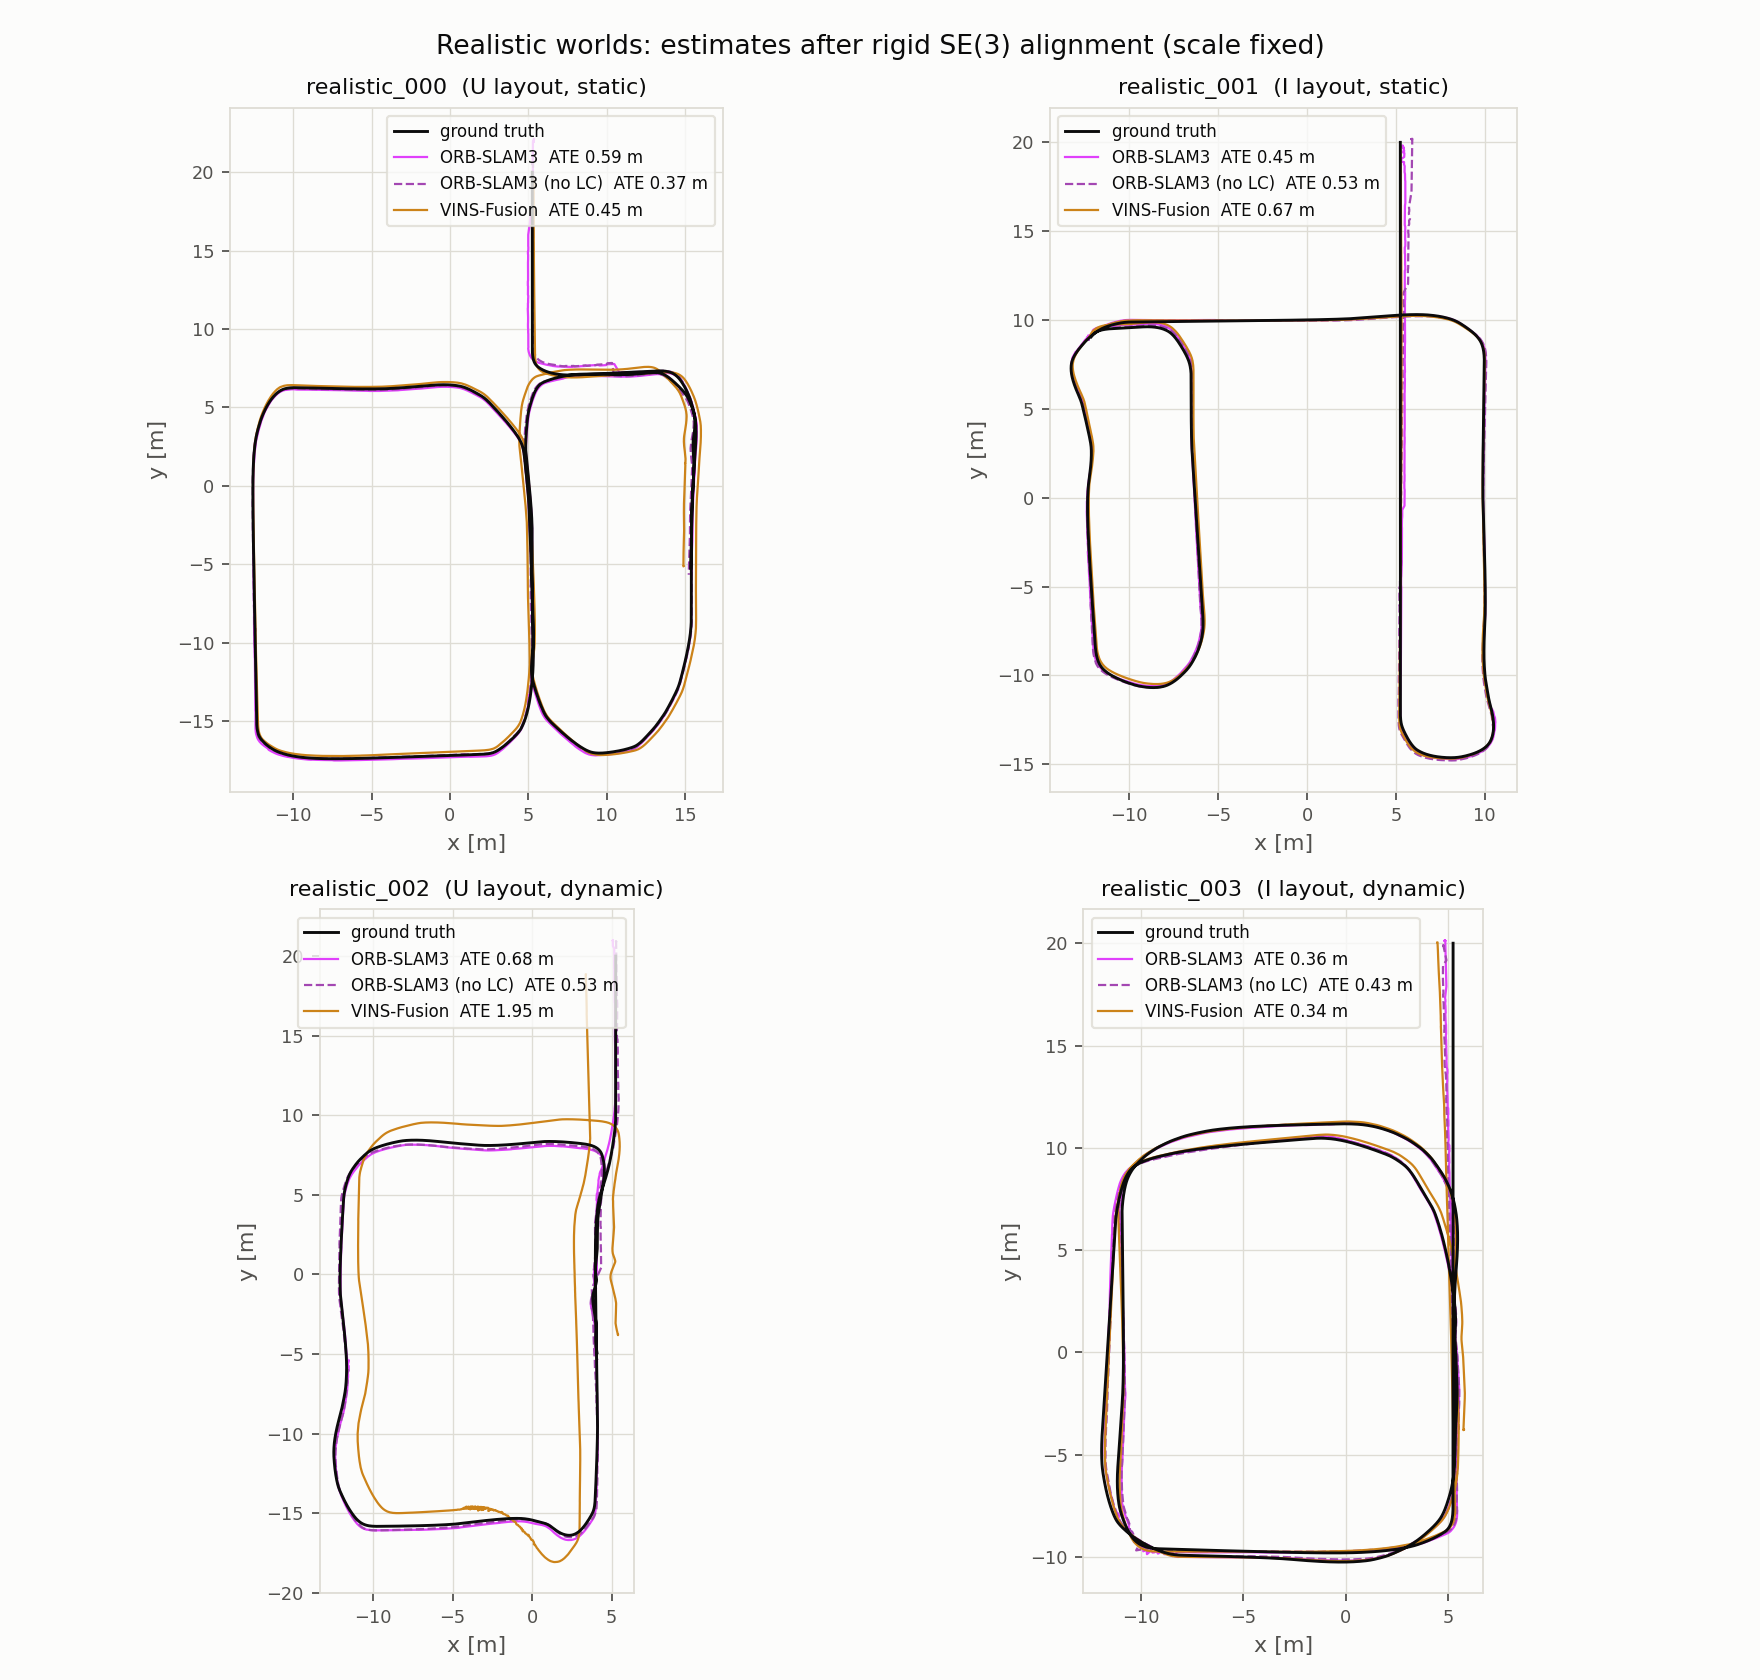
\includegraphics[width=0.92\textwidth]{figures/realistic_trajectories.png}
  \caption[Visual estimates on the four realistic recordings.]{Unfiltered
  estimates on the four realistic-warehouse recordings
  after rigid $SE(3)$ alignment with scale fixed, on the warehouse footprint.
  Top: the static twins; bottom: the same layouts with traffic. Solid magenta
  is ORB-SLAM3 with its loop closer active, dashed with it disabled, lighter
  for the GPU front end; orange is VINS-Fusion. The two excursions on
  \repo{realistic_001} are the loop-closing runs after their false closure;
  the \SI{1.4}{\metre} run on \repo{realistic_002} is the CPU loop-closing
  run; the closure-free runs on \repo{realistic_003} lie on the route in plan
  and diverge vertically.}
  \label{fig:realistic-traj}
\end{figure}

\begin{figure}[htbp]
  \centering
  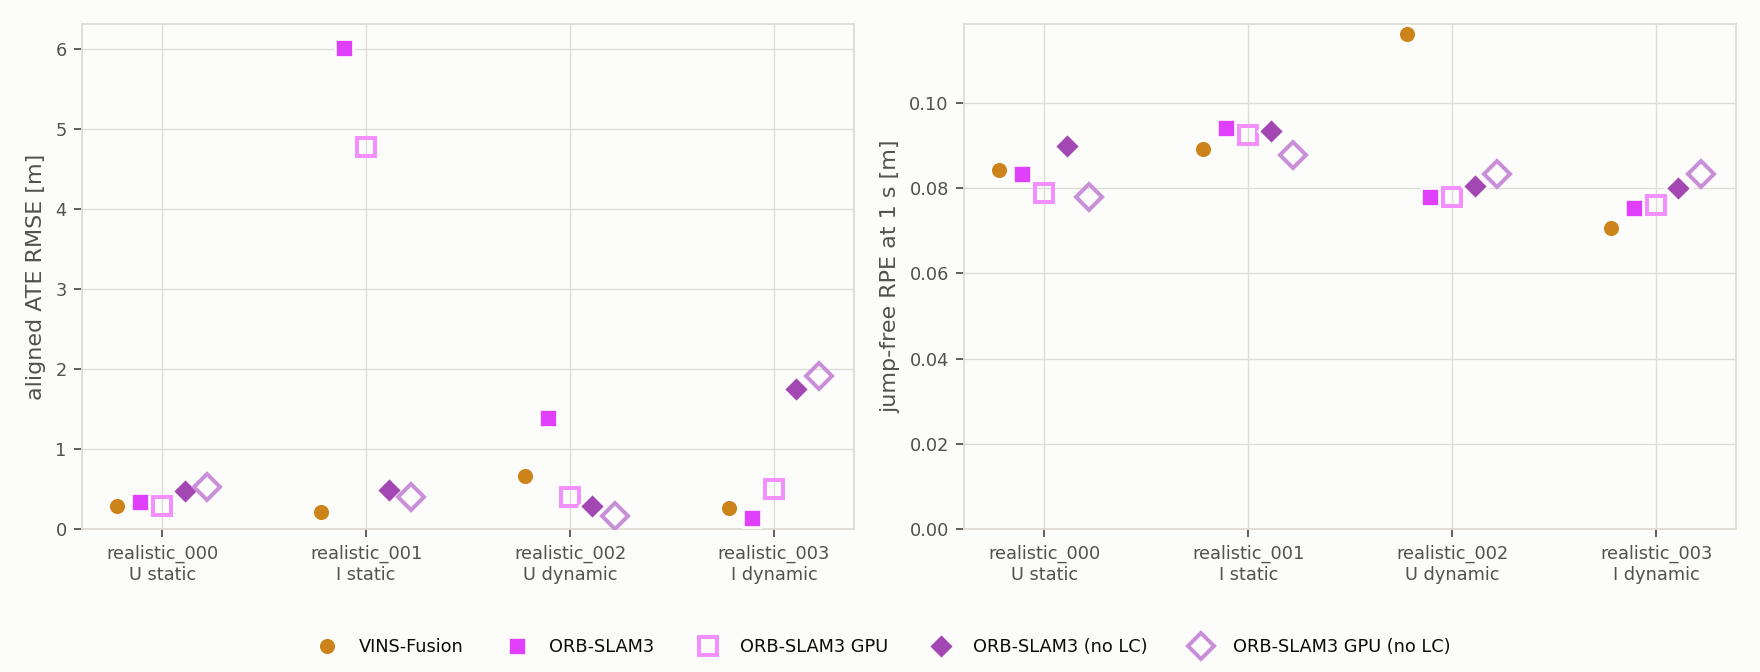
\includegraphics[width=\textwidth]{figures/realistic_metrics.png}
  \caption[Aligned ATE and jump-free RPE of the visual arms.]{Aligned ATE
  (left) and jump-free translational RPE at
  \SI{1}{\second} (right) of every visual run, one marker per run; filled
  markers are the CPU front end, open markers the GPU front end of the same
  configuration. The relative error is \SIrange{0.07}{0.12}{\metre} for every
  run, so the ATE differences are discrete events, not tracking quality.}
  \label{fig:realistic-metrics}
\end{figure}

\paragraph{Analysis: the loop closer decides, in both directions.} On the
static I layout both loop-closing runs accept one closure at \SI{73.2}{\second},
in the heading change at \SI{76}{\percent} of the route, with a correction of
\SI{14.7}{\metre} (CPU) and \SI{13.3}{\metre} (GPU) and \SIrange{1.9}{2.8}{\degree};
a global bundle adjustment follows and the trajectory is \SI{6.02}{} and
\SI{4.78}{\metre} off for the rest of the run, where the two closure-free runs
on the same recording hold \SI{0.50}{} and \SI{0.40}{\metre}
(\cref{fig:tl-real-001}). A route with half a metre of accumulated error
cannot need a fourteen-metre correction, so the match is false: the I layout's
long parallel aisles present the same rack faces twice, and the matched
keyframes (97 against 255, 104 against 272) are one aisle apart. The same
candidate was then re-proposed four times and rejected by the inertial
geometry check, after the damage. That both front ends accept it at the same
frame with the same correction says the place-recognition stage, not the
extractor, is where the fault lies.

On the I layout with traffic the sign reverses. Both loop-closing runs accept
one closure at \SI{56.5}{\second} (\SI{48}{\percent} of the route) with a
\SI{0.33}{\metre} correction and hold \SI{0.14}{} and \SI{0.50}{\metre}; the
closure-free runs read \SI{1.76}{} and \SI{1.91}{\metre}, yet their planar
error never exceeds \SI{0.7}{\metre} (\cref{fig:tl-real-003}). The difference
is vertical: the closure-free estimates climb to \SI{4.7}{} and
\SI{5.1}{\metre} above the floor by the end of the run while the loop-closing
runs stay within \SI{0.6}{} and \SI{1.4}{\metre}, and the three-dimensional
ATE reports that climb. The GPU loop-closing run on this recording also
rejected 148 further candidates by inertial geometry, every one of them after
its single accepted closure. On the U layout the closer is nearly inert: two
accepted closures per run on \repo{realistic_000} with corrections of
\SIrange{0.07}{0.12}{\metre}, one of \SIrange{0.26}{0.33}{\metre} per run on
\repo{realistic_002}, and the eight U-layout ORB-SLAM3 runs within
\SIrange{0.17}{0.52}{\metre} except the CPU loop-closing run on
\repo{realistic_002}, whose \SI{1.39}{\metre} is an offset present from
\SI{6.5}{\second} on, before any closure (\cref{fig:tl-real-002}); with four
jumps and the lowest relative error on the recording it is an initialisation
event, not a tracking one, and the GPU run of the same configuration, which
accepts the same closure at \SI{65}{\second}, does not reproduce it
(\SI{0.40}{\metre}).

\paragraph{Analysis: the front end changes throughput, not accuracy.} The GPU
extractor processes \SIrange{97}{99}{\percent} of each bag's frames where the
CPU extractor processes \SIrange{72}{94}{\percent}, and its tracking median
is \SIrange{30}{37}{\milli\second} against \SIrange{49}{55}{\milli\second}
(from the per-run \repo{performance.csv}). Across the eight CPU/GPU pairs
with the same closer state the ATE differs by at most \SI{0.16}{\metre} in
five; the three larger differences (\SI{-1.2}{}, \SI{-1.0}{} and
\SI{+0.4}{\metre}) are each one run's discrete event, in both directions,
and the two divergence patterns above occur in both front ends alike. At this frame budget the extractor is not the limiting
stage of accuracy on these recordings.

\paragraph{Analysis: traffic as a condition.} VINS-Fusion is \SI{0.37}{\metre}
worse on the U layout with traffic than on its static twin and \SI{0.05}{\metre}
worse on the I layout; its relative error on \repo{realistic_002} is the
highest of any run (\SI{0.116}{\metre}) and its error trace carries two
waves of \SI{0.7}{\metre} at \SI{25}{} and \SI{45}{\second} on the western and
southern aisles, where the pallet jacks work, that no static run shows
(\cref{fig:tl-real-002}). ORB-SLAM3's closure-free runs are \emph{better} on
the U traffic recording (\SI{0.29}{}, \SI{0.17}{\metre}) than on its static
twin (\SI{0.48}{}, \SI{0.52}{\metre}). With one run per cell and routes that
differ between twin and traffic recording, neither number is a traffic effect;
what the slot establishes is that physically simulated traffic degrades the
tracker that follows features longest, and breaks neither.

\paragraph{Analysis: the two estimators err in perpendicular directions.}
VINS-Fusion drifts sideways and ORB-SLAM3 drifts forwards, which the aligned
ATE cannot show. Decomposing each run's error in the ground-truth heading frame
(% Generated by script/exp1_error_pattern.py -- do not edit by hand.
\begin{table}[htbp]
\centering
\caption[Translation error of the visual arms, split by direction.]{Translation error of the visual arms split in the ground-truth heading frame, on the same aligned series the reported ATE is computed from, so that the parts account for the whole. ``Along'' is the component along the truth's heading and ``cross'' the one perpendicular to it; ``bias'' is the mean of the signed component, so a bias near the RMS means a constant offset rather than scatter. ``Cross share'' is the cross-track fraction of the planar squared error: \num{0.5} is isotropic and above it the estimate drifts sideways, which is the direction that matters in a \SI{3.0}{\metre} aisle. One run per cell; ORB-SLAM3's run-to-run spread reaches \SI{0.277}{\metre}, so differences smaller than that between single runs are not evidence.}
\label{tab:exp1-translation-pattern}
\small
\resizebox{\textwidth}{!}{%
\begin{tabular}{llrrrrrrr}
\toprule
Recording & Estimator & ATE [\si{\metre}] & Along [\si{\metre}] & Cross [\si{\metre}] & Vert.\ [\si{\metre}] & Along bias & Cross bias & Cross share \\
\midrule
\repo{realistic_000} & VINS-Fusion & 0.290 & 0.148 & 0.211 & 0.133 & -0.028 & +0.074 & 0.67 \\
 & ORB-SLAM3 & 0.338 & 0.281 & 0.095 & 0.162 & -0.072 & +0.029 & 0.10 \\
 & ORB-SLAM3 GPU & 0.293 & 0.237 & 0.093 & 0.145 & -0.077 & +0.019 & 0.13 \\
 & ORB-SLAM3 (no LC) & 0.483 & 0.412 & 0.185 & 0.171 & -0.098 & +0.035 & 0.17 \\
 & ORB-SLAM3 GPU (no LC) & 0.523 & 0.422 & 0.263 & 0.161 & -0.073 & +0.063 & 0.28 \\
\addlinespace
\repo{realistic_001} & VINS-Fusion & 0.221 & 0.070 & 0.107 & 0.180 & -0.011 & -0.044 & 0.70 \\
 & ORB-SLAM3 & 6.021 & 3.687 & 4.756 & 0.213 & -1.598 & -1.372 & 0.62 \\
 & ORB-SLAM3 GPU & 4.780 & 2.644 & 3.978 & 0.182 & -0.909 & -1.166 & 0.69 \\
 & ORB-SLAM3 (no LC) & 0.496 & 0.259 & 0.093 & 0.413 & -0.079 & +0.036 & 0.11 \\
 & ORB-SLAM3 GPU (no LC) & 0.400 & 0.196 & 0.046 & 0.346 & -0.051 & +0.022 & 0.05 \\
\addlinespace
\repo{realistic_002} & VINS-Fusion & 0.663 & 0.236 & 0.091 & 0.613 & -0.019 & +0.030 & 0.13 \\
 & ORB-SLAM3 & 1.393 & 1.311 & 0.454 & 0.118 & -0.297 & +0.044 & 0.11 \\
 & ORB-SLAM3 GPU & 0.400 & 0.328 & 0.148 & 0.175 & -0.081 & -0.008 & 0.17 \\
 & ORB-SLAM3 (no LC) & 0.293 & 0.222 & 0.100 & 0.163 & +0.001 & -0.048 & 0.17 \\
 & ORB-SLAM3 GPU (no LC) & 0.170 & 0.100 & 0.051 & 0.127 & -0.002 & -0.032 & 0.21 \\
\addlinespace
\repo{realistic_003} & VINS-Fusion & 0.268 & 0.101 & 0.167 & 0.184 & +0.035 & +0.020 & 0.73 \\
 & ORB-SLAM3 & 0.139 & 0.070 & 0.042 & 0.112 & -0.011 & -0.012 & 0.26 \\
 & ORB-SLAM3 GPU & 0.504 & 0.104 & 0.045 & 0.491 & -0.003 & -0.022 & 0.16 \\
 & ORB-SLAM3 (no LC) & 1.755 & 0.072 & 0.071 & 1.752 & -0.014 & -0.005 & 0.50 \\
 & ORB-SLAM3 GPU (no LC) & 1.911 & 0.199 & 0.114 & 1.897 & -0.042 & +0.016 & 0.25 \\
\bottomrule
\end{tabular}}
\end{table}
, \cref{fig:exp1-translation-pattern}),
VINS-Fusion's cross-track share of the planar error is
\numrange{0.67}{0.73} on three of the four recordings while every ORB-SLAM3 run
that held tracking lies between \num{0.11} and \num{0.25}. On
\repo{realistic_000} the two score \SI{0.293}{} and \SI{0.290}{\metre}:
indistinguishable, and perpendicular. For a \num{0.83} by \SI{0.50}{\metre}
robot in a \SI{3.0}{\metre} aisle they are not equally safe, because
cross-track error closes the gap to the racking and along-track error does not.

The false closure is also the failure that throws the estimate sideways. The
two loop-closing runs on \repo{realistic_001} are the only ORB-SLAM3 runs whose
cross-track share exceeds \num{0.5} (\num{0.62} and \num{0.69}), with
cross-track RMS of \SI{4.76}{} and \SI{3.98}{\metre}; of the five diverged runs
only those two are cross-track dominated, so the direction belongs to the false
closure and not to divergence in general. The error is scatter rather than
offset throughout: the mean of each signed component is
\numrange{0.17}{0.36} of its RMS in every arm. Both decompositions are computed
on the same aligned series the reported ATE uses, so the parts account for the
whole, and both are pooled over the twenty runs rather than ranked, because one
run per cell cannot separate arms that differ by less than ORB-SLAM3's
\SI{0.277}{\metre} run-to-run spread.

\paragraph{Analysis: the rotation column.} ORB-SLAM3's \SIrange{13}{19}{\degree}
rotational RMSE is one event on every run: the first jump lies at
\SIrange{2.5}{4.8}{\second} (\cref{tab:realistic-timelines-baseline}), where
inertial initialisation re-aligns the world frame to gravity, and after it the
clean rotational RPE is \SIrange{0.07}{0.33}{\degree}. The jump detector is
translational, so the column includes the event; the median is the number to
read. Splitting the error by axis confirms what kind of event it is
(% Generated by script/exp1_error_pattern.py -- do not edit by hand.
\begin{table}[htbp]
\centering
\caption[Orientation error of the visual arms, by axis and by turn rate.]{Orientation error of the visual arms. Yaw, pitch and roll are the wrapped per-axis differences between the aligned estimate and the truth; for a robot on a flat floor a sustained pitch or roll error is a gravity-alignment defect rather than drift. The median is given beside the RMS because the RMS of an ORB-SLAM3 run is dominated by the single re-alignment at its inertial initialisation. ``Turning'' is a ground-truth turn rate above \SI{10}{\degree\per\second}, the threshold the onset analysis uses; the two medians are paired within a run. One run per cell.}
\label{tab:exp1-rotation-pattern}
\small
\resizebox{\textwidth}{!}{%
\begin{tabular}{llrrrrrrr}
\toprule
Recording & Estimator & Yaw [\si{\degree}] & Pitch [\si{\degree}] & Roll [\si{\degree}] & Rot.\ RMS & Rot.\ med. & Med.\ turning & Med.\ straight \\
\midrule
\repo{realistic_000} & VINS-Fusion & 0.45 & 1.20 & 1.34 & 1.85 & 0.85 & 0.80 & 0.89 \\
 & ORB-SLAM3 & 23.60 & 13.66 & 23.58 & 13.74 & 0.28 & 0.30 & 0.28 \\
 & ORB-SLAM3 GPU & 18.75 & 12.75 & 18.71 & 12.80 & 0.33 & 0.37 & 0.32 \\
 & ORB-SLAM3 (no LC) & 19.99 & 14.01 & 19.98 & 14.05 & 0.25 & 0.28 & 0.25 \\
 & ORB-SLAM3 GPU (no LC) & 23.26 & 12.74 & 23.27 & 12.84 & 0.49 & 0.48 & 0.49 \\
\addlinespace
\repo{realistic_001} & VINS-Fusion & 0.24 & 0.90 & 0.72 & 1.18 & 0.93 & 0.86 & 0.96 \\
 & ORB-SLAM3 & 24.27 & 15.16 & 24.39 & 16.92 & 6.83 & 6.82 & 6.83 \\
 & ORB-SLAM3 GPU & 26.16 & 14.55 & 24.24 & 18.98 & 6.57 & 6.58 & 6.56 \\
 & ORB-SLAM3 (no LC) & 17.02 & 15.05 & 17.31 & 16.05 & 3.52 & 3.44 & 3.52 \\
 & ORB-SLAM3 GPU (no LC) & 17.08 & 14.43 & 17.19 & 15.13 & 2.62 & 2.61 & 2.62 \\
\addlinespace
\repo{realistic_002} & VINS-Fusion & 0.21 & 1.65 & 3.15 & 3.57 & 2.74 & 2.55 & 2.77 \\
 & ORB-SLAM3 & 2.06 & 16.95 & 1.93 & 16.99 & 1.31 & 1.33 & 1.30 \\
 & ORB-SLAM3 GPU & 14.51 & 15.94 & 14.46 & 16.04 & 0.59 & 0.62 & 0.56 \\
 & ORB-SLAM3 (no LC) & 19.80 & 17.02 & 19.75 & 17.12 & 0.62 & 0.65 & 0.60 \\
 & ORB-SLAM3 GPU (no LC) & 12.13 & 16.05 & 12.09 & 16.08 & 0.34 & 0.44 & 0.32 \\
\addlinespace
\repo{realistic_003} & VINS-Fusion & 0.24 & 0.70 & 1.31 & 1.51 & 1.04 & 0.99 & 1.06 \\
 & ORB-SLAM3 & 14.97 & 13.44 & 14.91 & 13.52 & 0.45 & 0.47 & 0.44 \\
 & ORB-SLAM3 GPU & 10.39 & 12.99 & 10.49 & 13.16 & 1.39 & 1.61 & 1.24 \\
 & ORB-SLAM3 (no LC) & 15.56 & 13.70 & 15.70 & 14.22 & 2.24 & 2.07 & 2.24 \\
 & ORB-SLAM3 GPU (no LC) & 13.54 & 13.04 & 13.68 & 13.53 & 2.54 & 2.60 & 2.52 \\
\bottomrule
\end{tabular}}
\end{table}
, \cref{fig:exp1-rotation-pattern}): yaw,
pitch and roll RMS are all \SIrange{14}{19}{\degree} while their medians are
\SIrange{0.88}{1.51}{\degree}, and an error that moves all three axes together
and persists in none is a frame re-alignment rather than drift. Turning does
not raise the rotation error either: pooled over the twenty runs the median
while turning exceeds the median while straight by \SI{+0.01}{\degree}, and
eleven of twenty runs are positive, which is a coin flip. VINS-Fusion carries a
smaller signature of the same kind, pitch and roll RMS of \SI{1.05}{} and
\SI{1.33}{\degree} against a yaw RMS of \SI{0.24}{\degree};
\flag{whether that is a residual gravity error or the rigid fit absorbing a
tilt has not been separated, and it is reported as an observation.}

% Generated by script/analyse_exp3_timelines.py -- do not edit by hand.
\begin{table}[htbp]
\centering
\caption{Realistic world, unfiltered runs: onset of sustained error and its place on the route, per run, under the same definitions as \cref{tab:realistic-timelines-filtered}. One entry per run, in repeat order; ``never'' means the error stayed below the threshold for the whole run.}
\label{tab:realistic-timelines-baseline}
\scriptsize
\resizebox{\textwidth}{!}{%
\begin{tabular}{lll l l}
\toprule
Recording & Estimator & LC & Onset [\si{\second}] (where) & First jump [\si{\second}] \\
\midrule
\repo{realistic_000} & ORB-SLAM3 & active & never & 6 \\
 & ORB-SLAM3 & disabled & never & 6 \\
 & VINS-Fusion & --- & 110 (straight 90\,\%) & --- \\
\repo{realistic_001} & ORB-SLAM3 & active & never & --- \\
 & ORB-SLAM3 & disabled & never & 5 \\
 & VINS-Fusion & --- & never & --- \\
\repo{realistic_002} & ORB-SLAM3 & active & never & 3 \\
 & ORB-SLAM3 & disabled & never & 3 \\
 & VINS-Fusion & --- & 30 (turn 39\,\%) & --- \\
\repo{realistic_003} & ORB-SLAM3 & active & never & 4 \\
 & ORB-SLAM3 & disabled & never & 3 \\
 & VINS-Fusion & --- & never & --- \\
\bottomrule
\end{tabular}}
\end{table}


\begin{figure}[p]
  \centering
  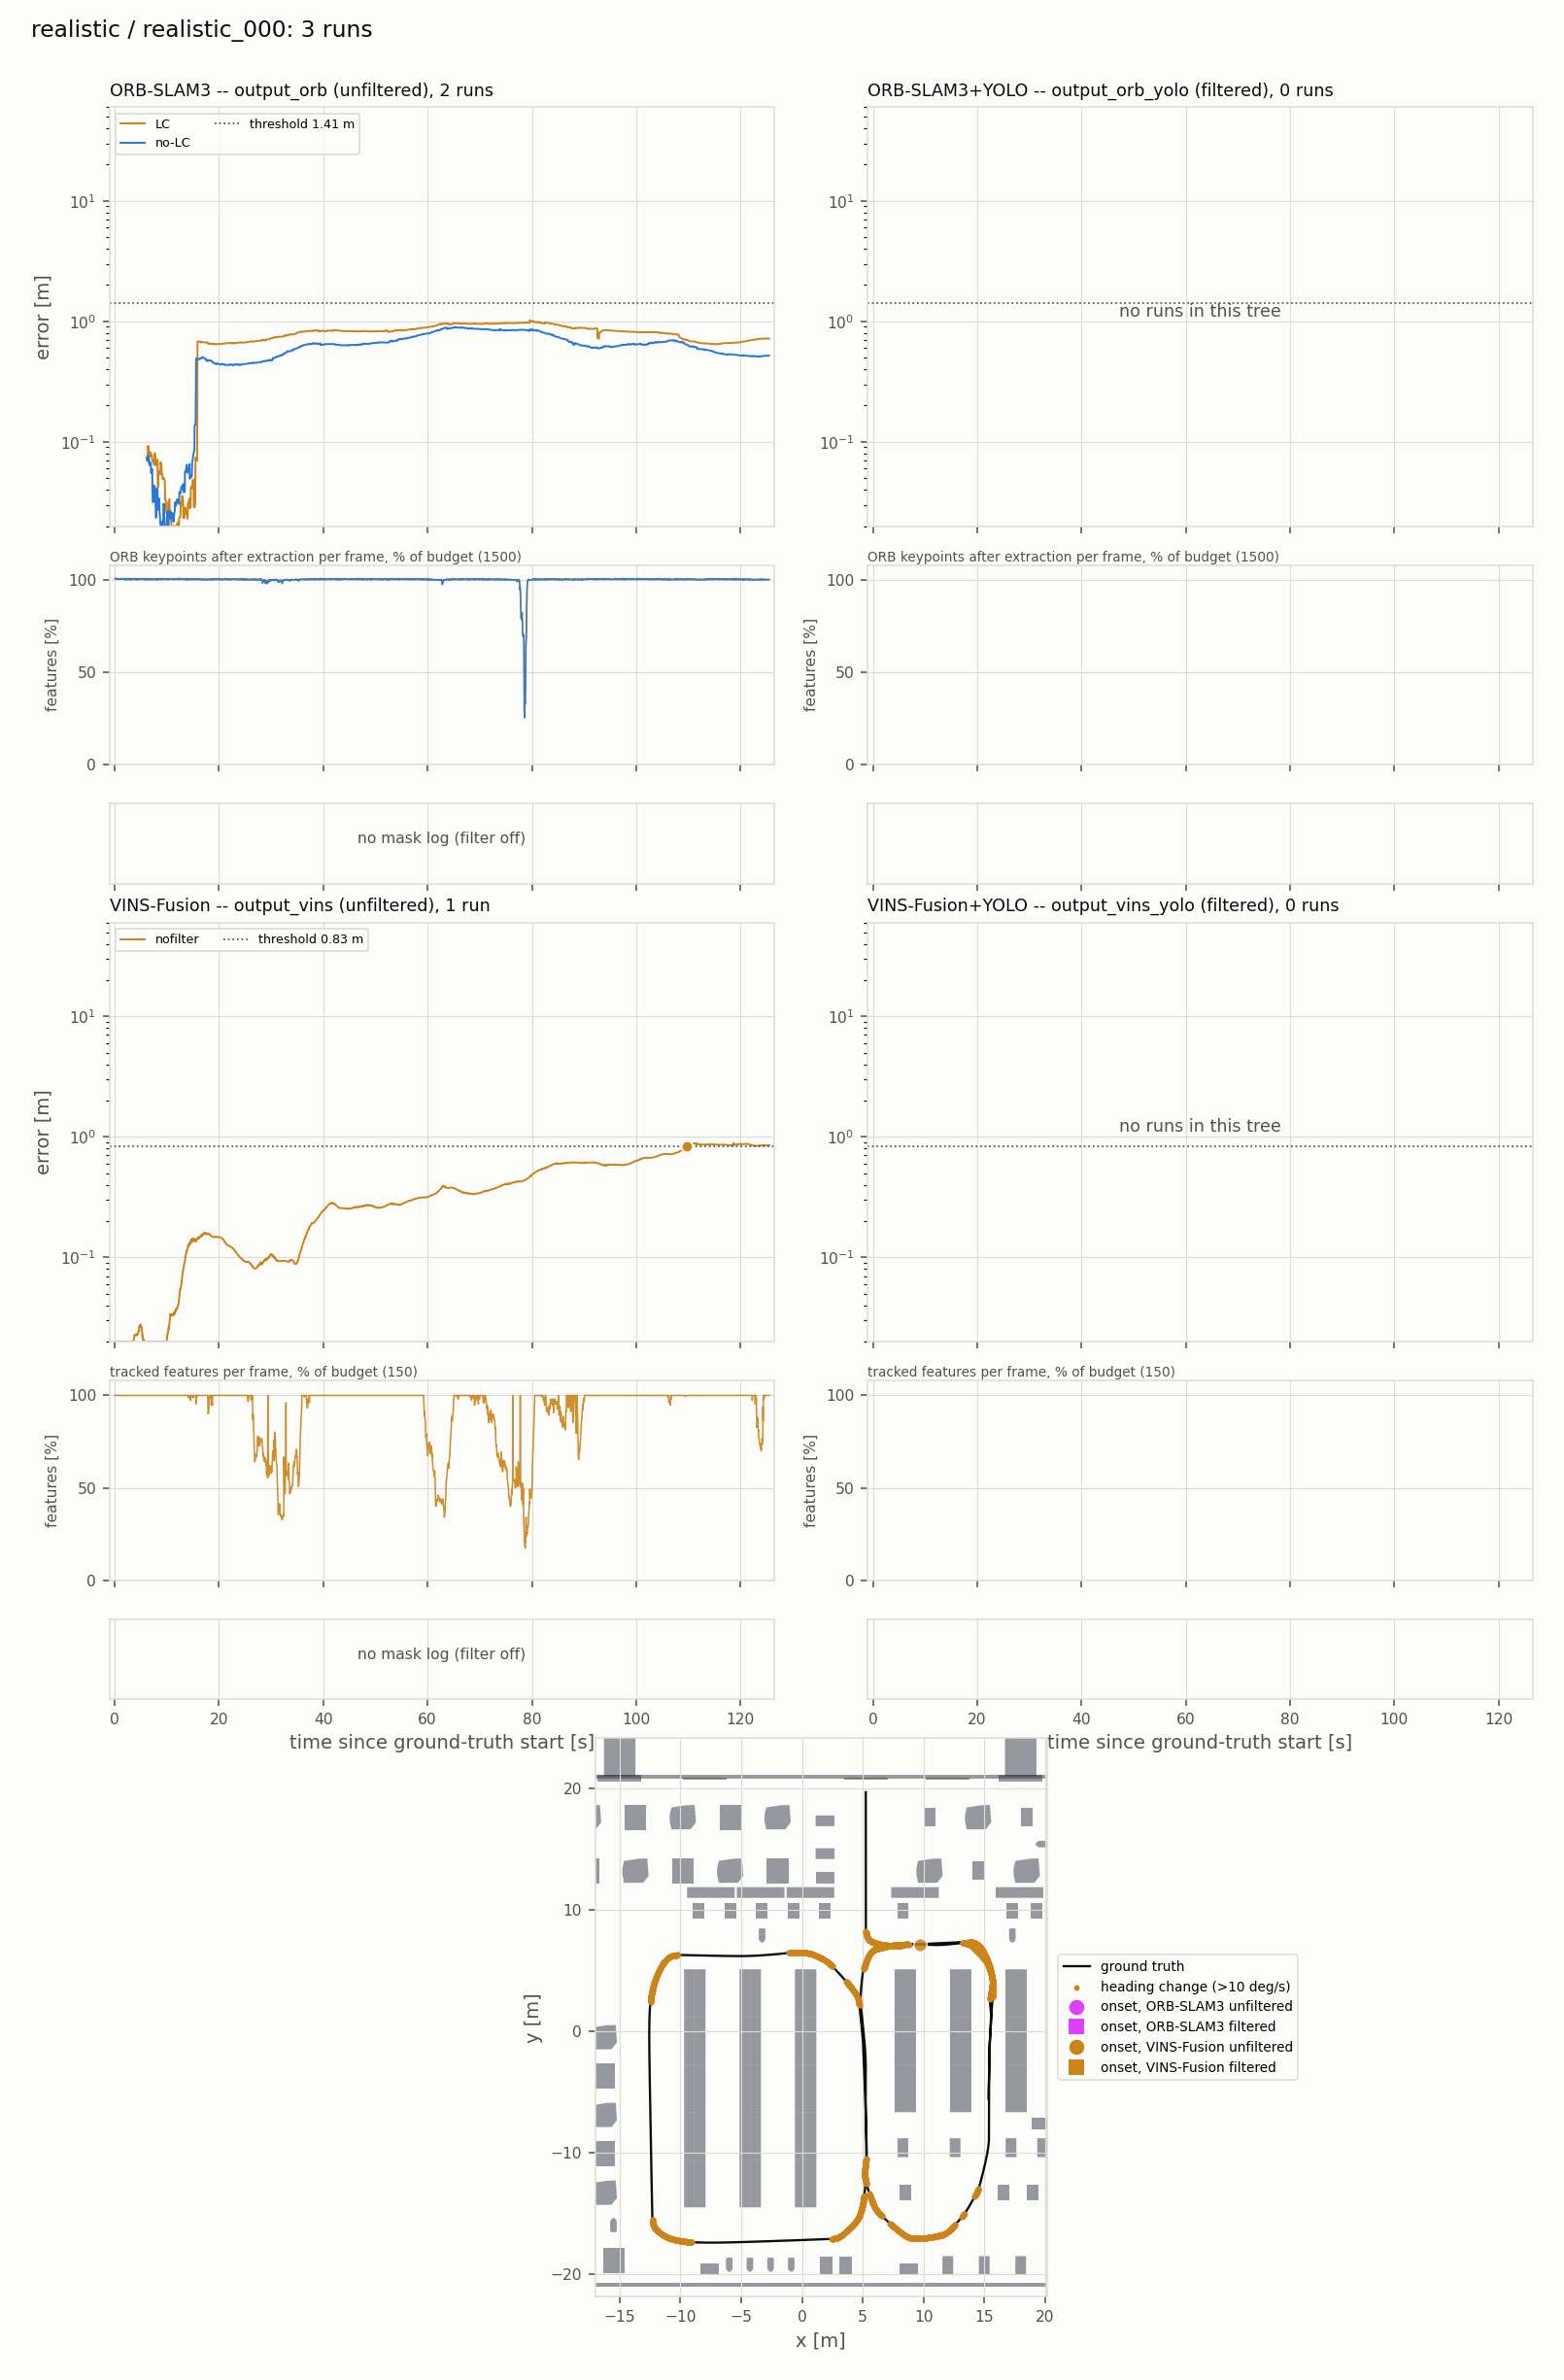
\includegraphics[width=0.98\textwidth]{figures/timeline_realistic__realistic_000.png}
  \caption[Timelines, static U-layout recording.]{\repo{realistic_000} (U,
  static), every run. Left: start-anchored
  planar error on a log axis, solid for loop closing active, dotted for
  disabled, lighter for the GPU front end, with each estimator's threshold;
  the dot marks the onset of sustained excess. Right: the route with heading
  changes in orange and every onset placed on it. The one onset is the GPU
  closure-free run at \SI{60}{\second}, a sustained \SI{1.3}{\metre} offset on
  the straight, not a jump.}
  \label{fig:tl-real-000}
\end{figure}
\begin{figure}[p]
  \centering
  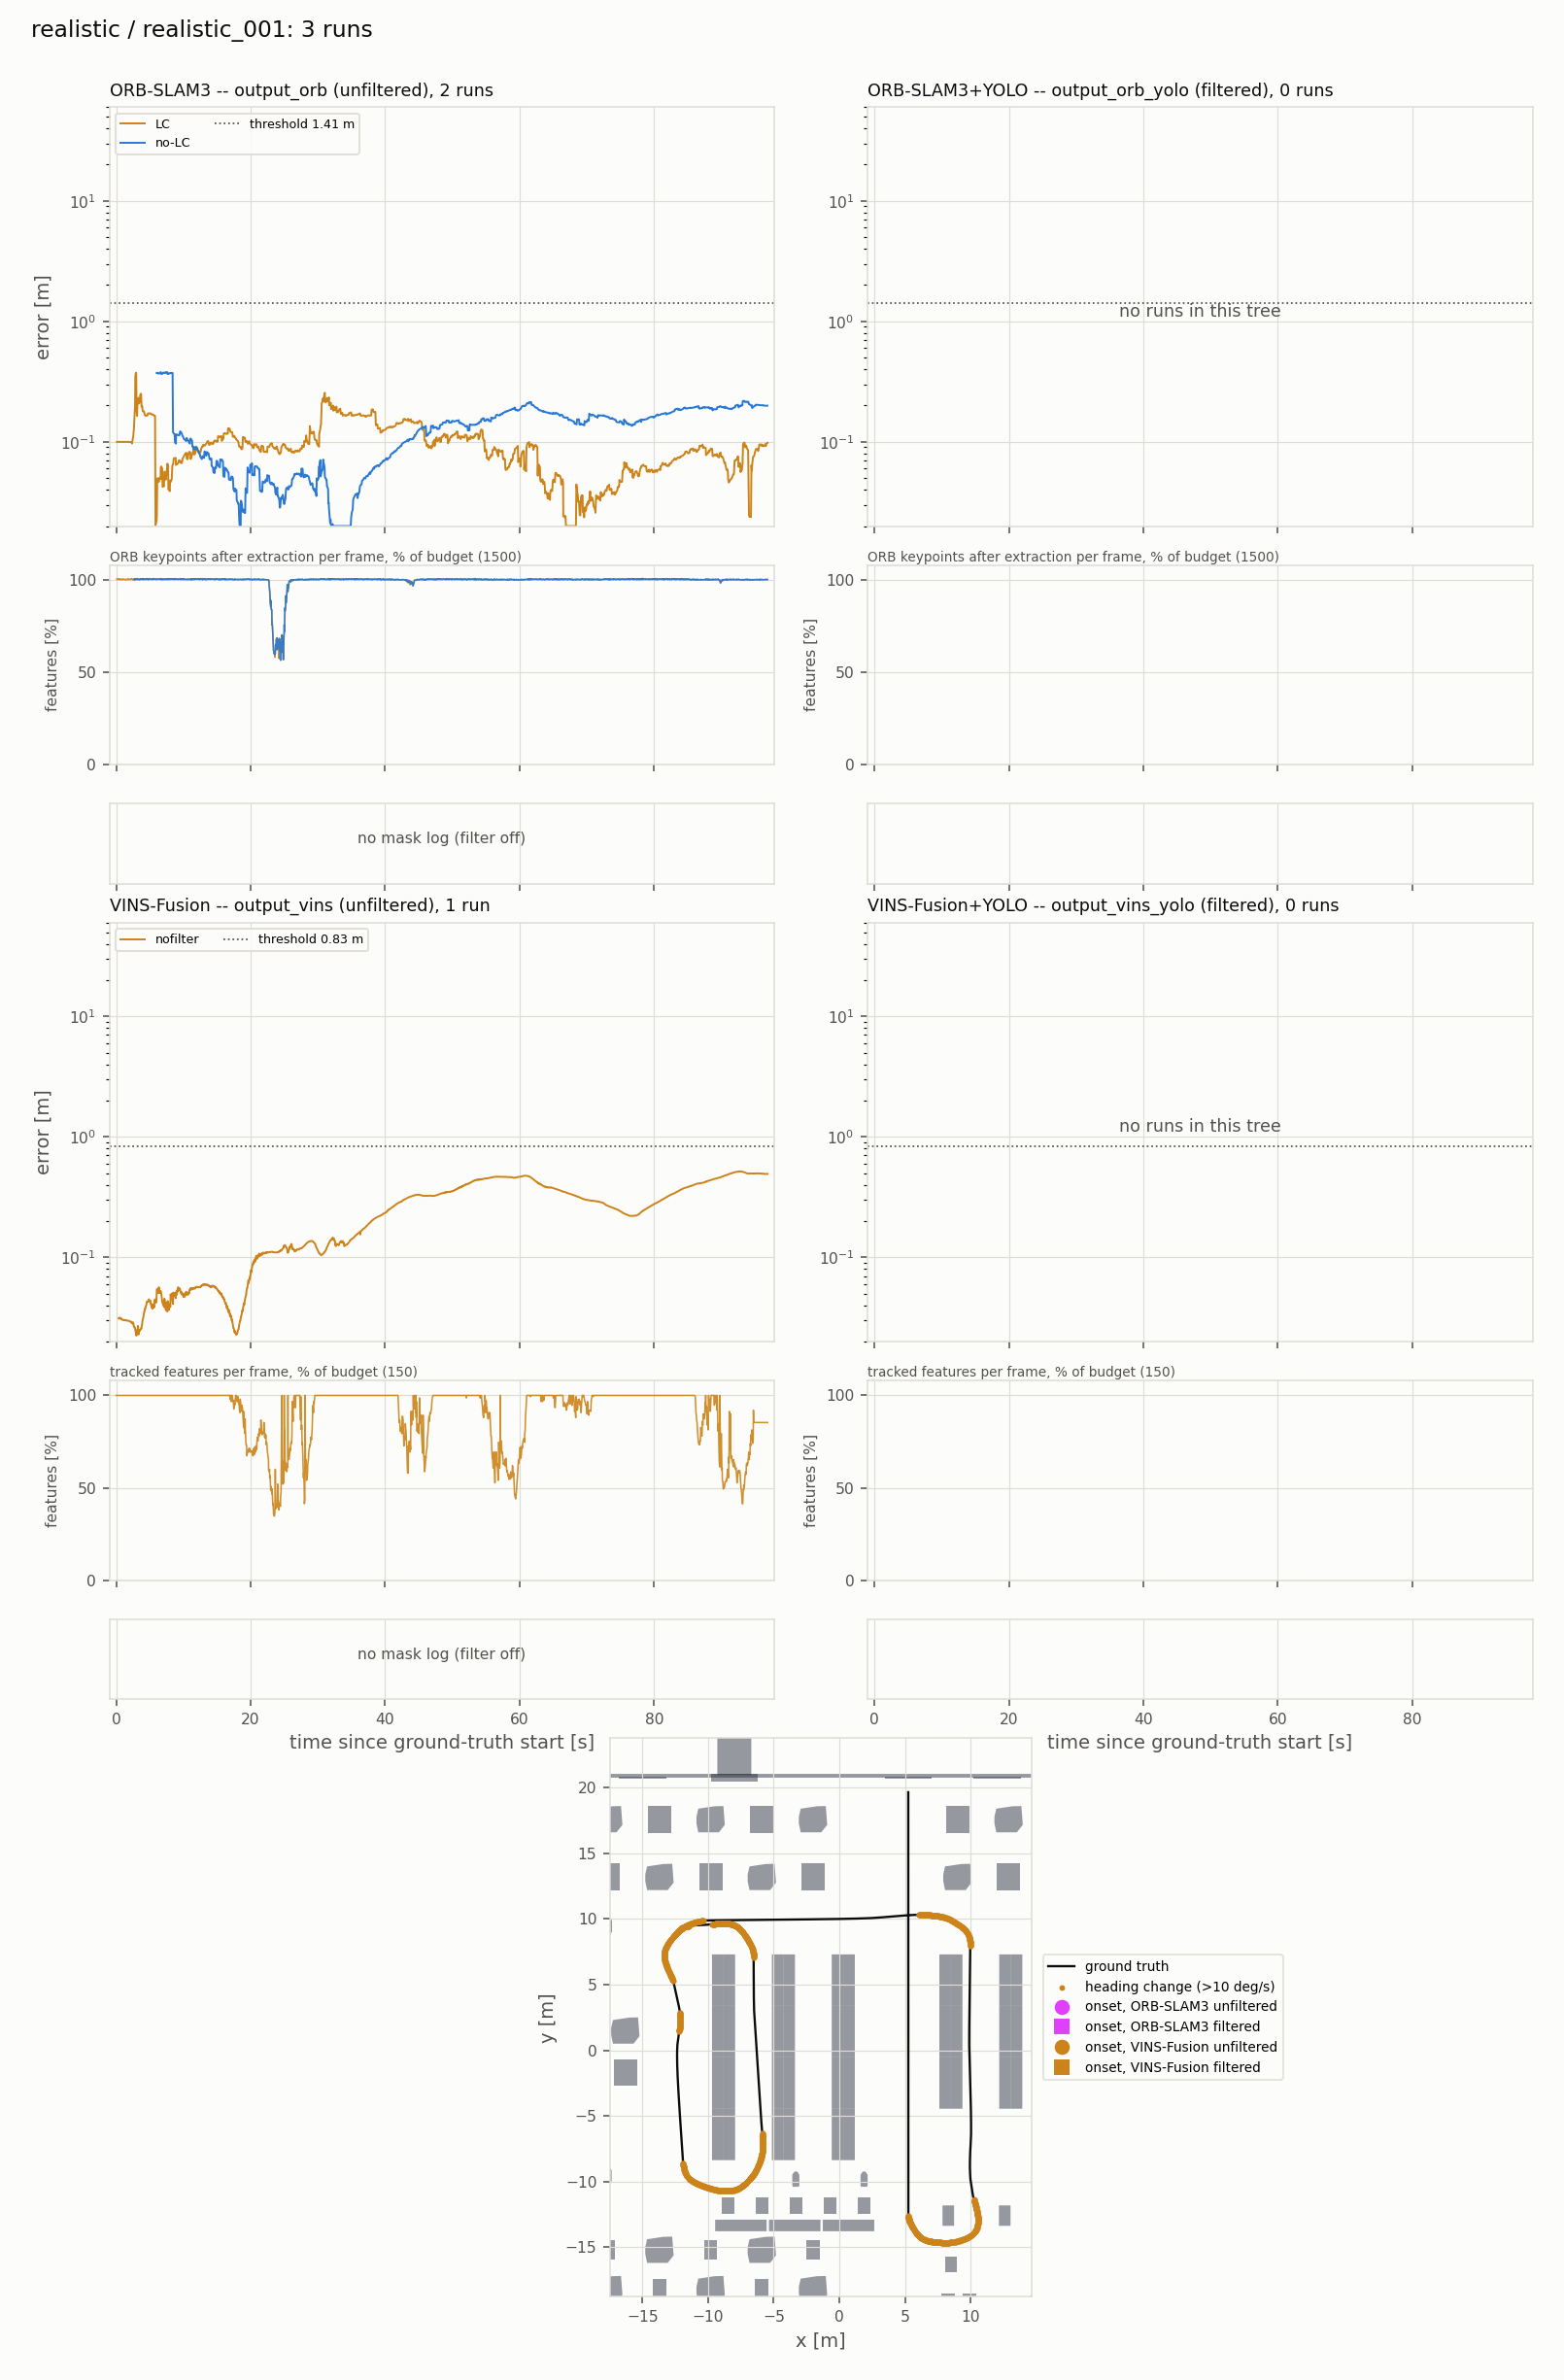
\includegraphics[width=0.98\textwidth]{figures/timeline_realistic__realistic_001.png}
  \caption[Timelines, static I-layout recording.]{\repo{realistic_001} (I,
  static), every run; panels as in
  \cref{fig:tl-real-000}. Both loop-closing runs step to \SI{14}{\metre} of
  error at \SI{73}{\second}, in the heading change at \SI{76}{\percent} of the
  route, at the single accepted closure; the closure-free runs and VINS-Fusion
  never cross.}
  \label{fig:tl-real-001}
\end{figure}
\begin{figure}[p]
  \centering
  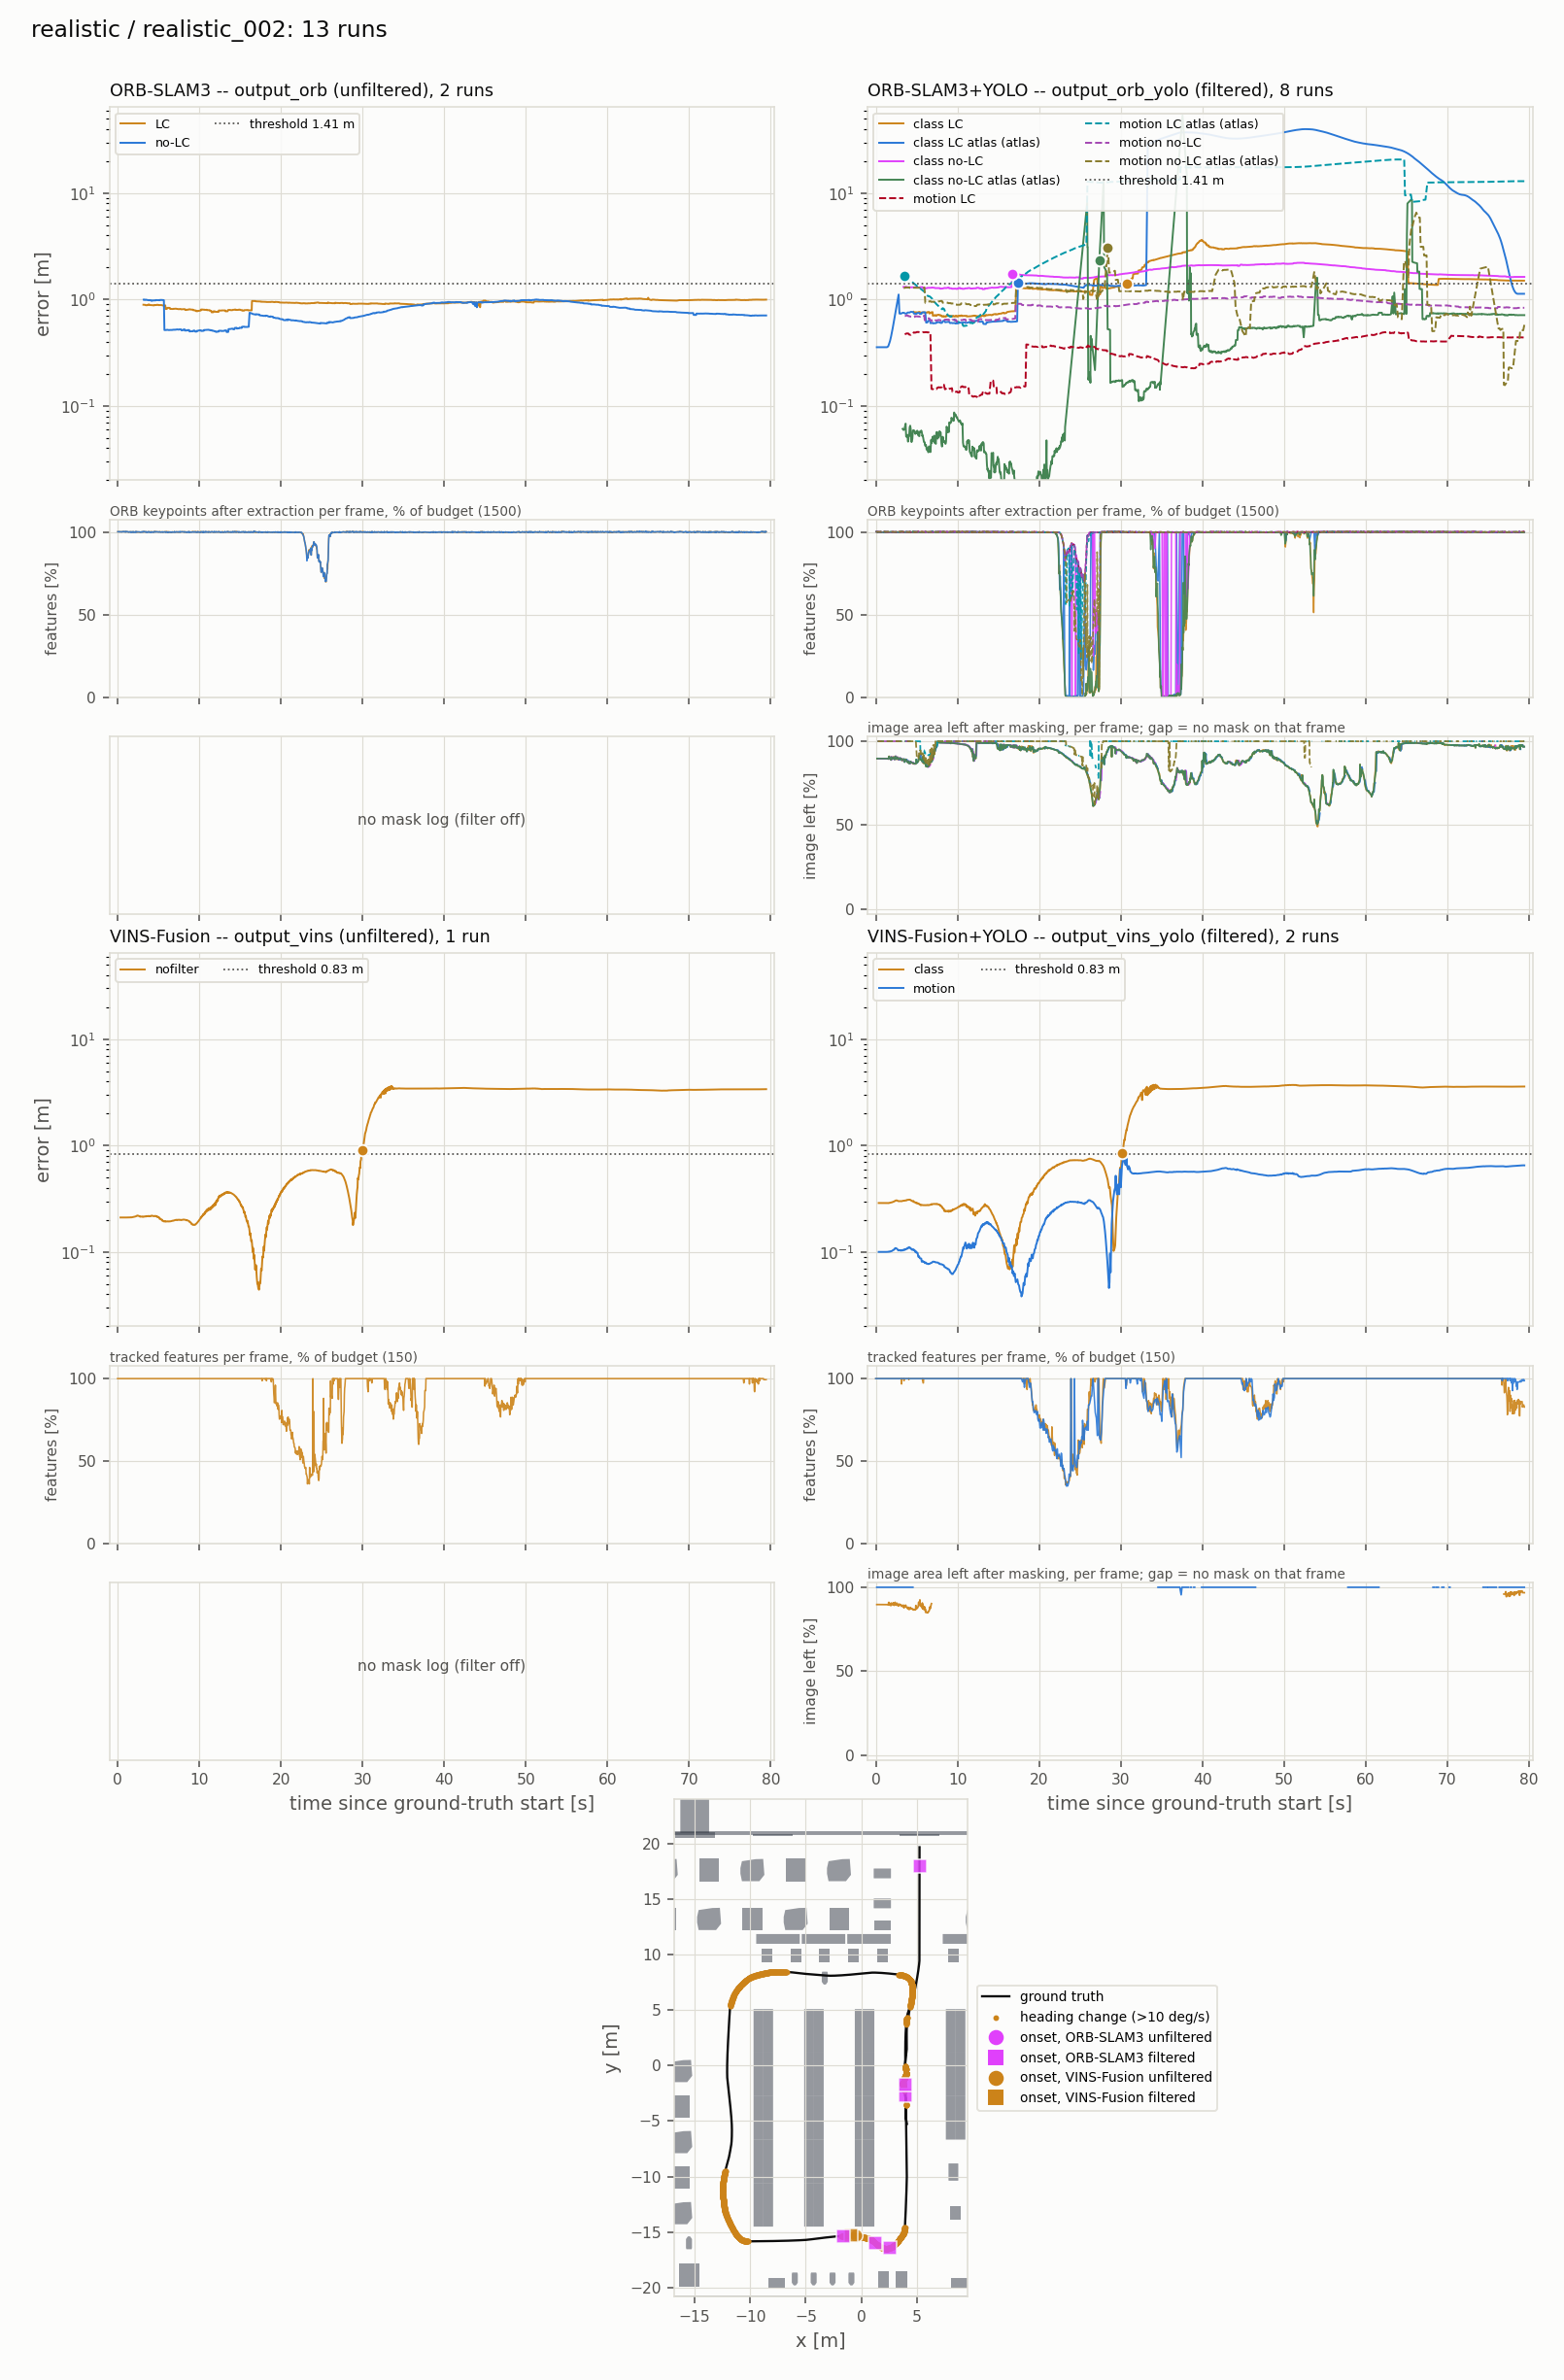
\includegraphics[width=0.98\textwidth]{figures/timeline_realistic__realistic_002.png}
  \caption[Timelines, U-layout recording with traffic.]{\repo{realistic_002}
  (U, traffic), every run; panels as in
  \cref{fig:tl-real-000}. The CPU loop-closing run carries a \SI{1.5}{\metre}
  offset from \SI{6.5}{\second}, which the GPU loop-closing run does not
  share; VINS-Fusion's two \SI{0.7}{\metre} waves at \SI{25}{} and
  \SI{45}{\second} lie on the aisles where the pallet jacks work.}
  \label{fig:tl-real-002}
\end{figure}
\begin{figure}[p]
  \centering
  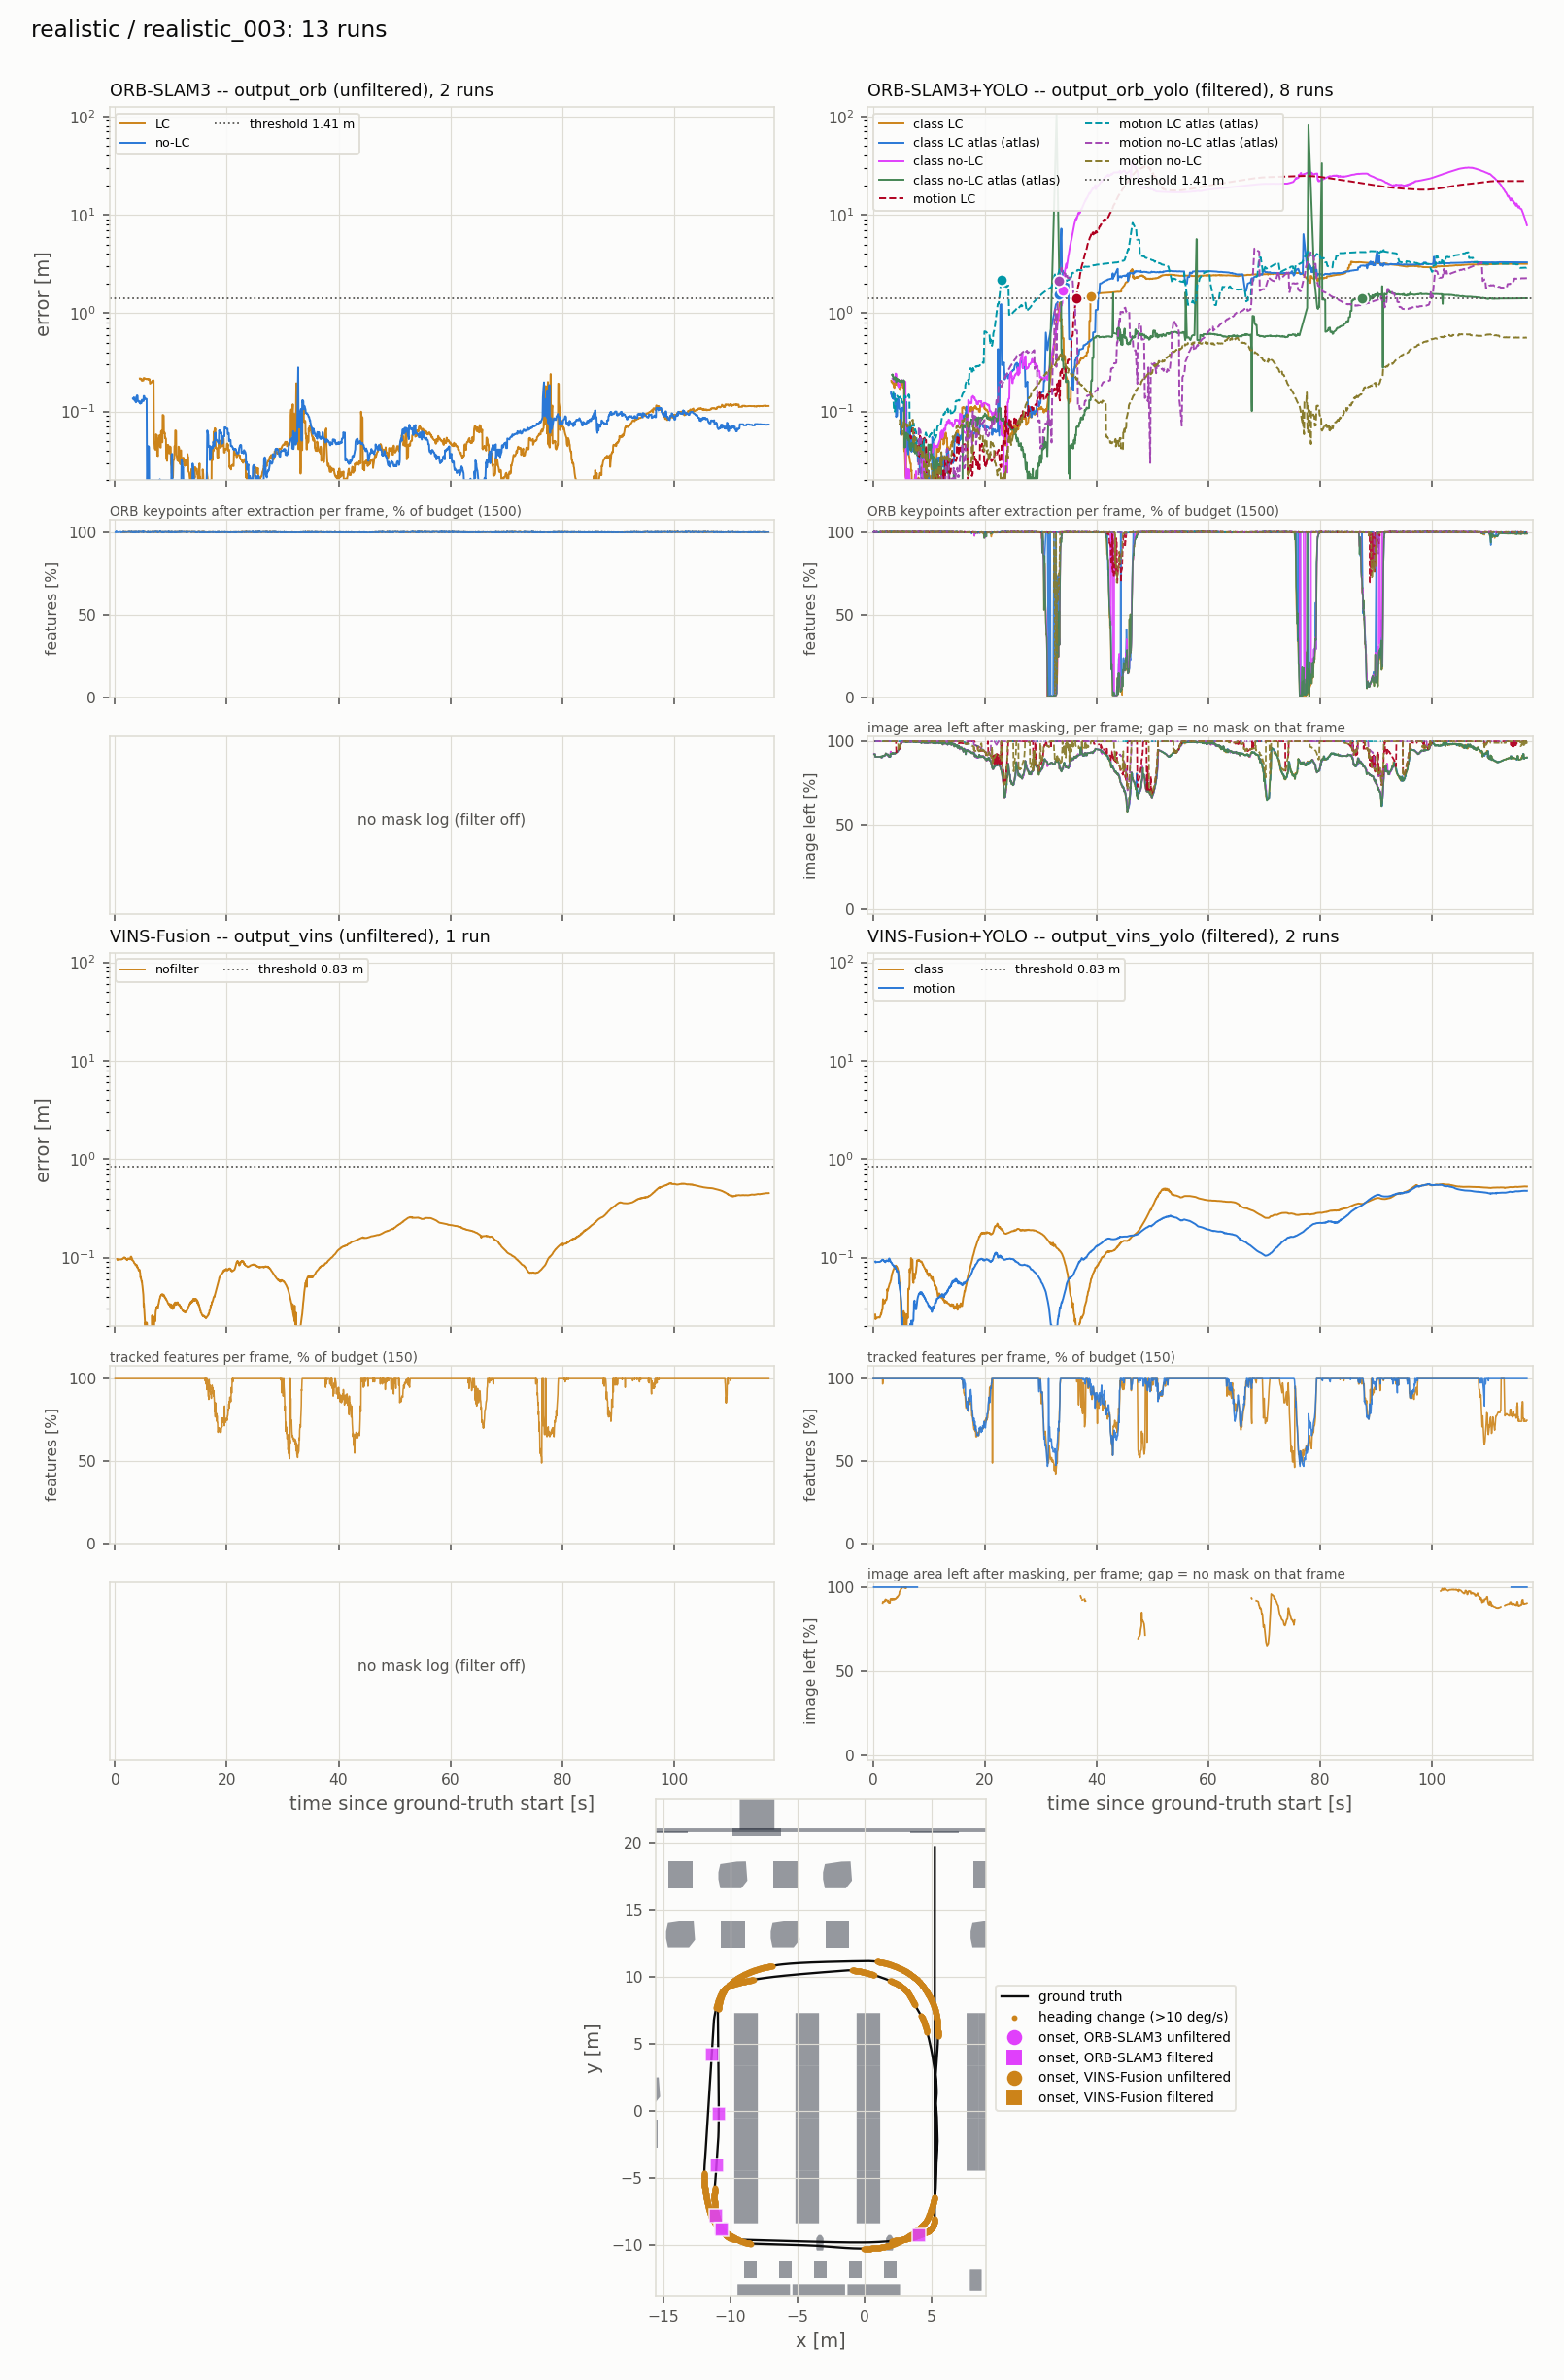
\includegraphics[width=0.98\textwidth]{figures/timeline_realistic__realistic_003.png}
  \caption[Timelines, I-layout recording with traffic.]{\repo{realistic_003}
  (I, traffic), every run; panels as in
  \cref{fig:tl-real-000}. No run crosses its threshold in the plane; the
  \SI{1.8}{} and \SI{1.9}{\metre} ATE of the closure-free runs is vertical
  drift, which the single accepted closure of the loop-closing runs removes.}
  \label{fig:tl-real-003}
\end{figure}

\begin{figure}[p]
  \centering
  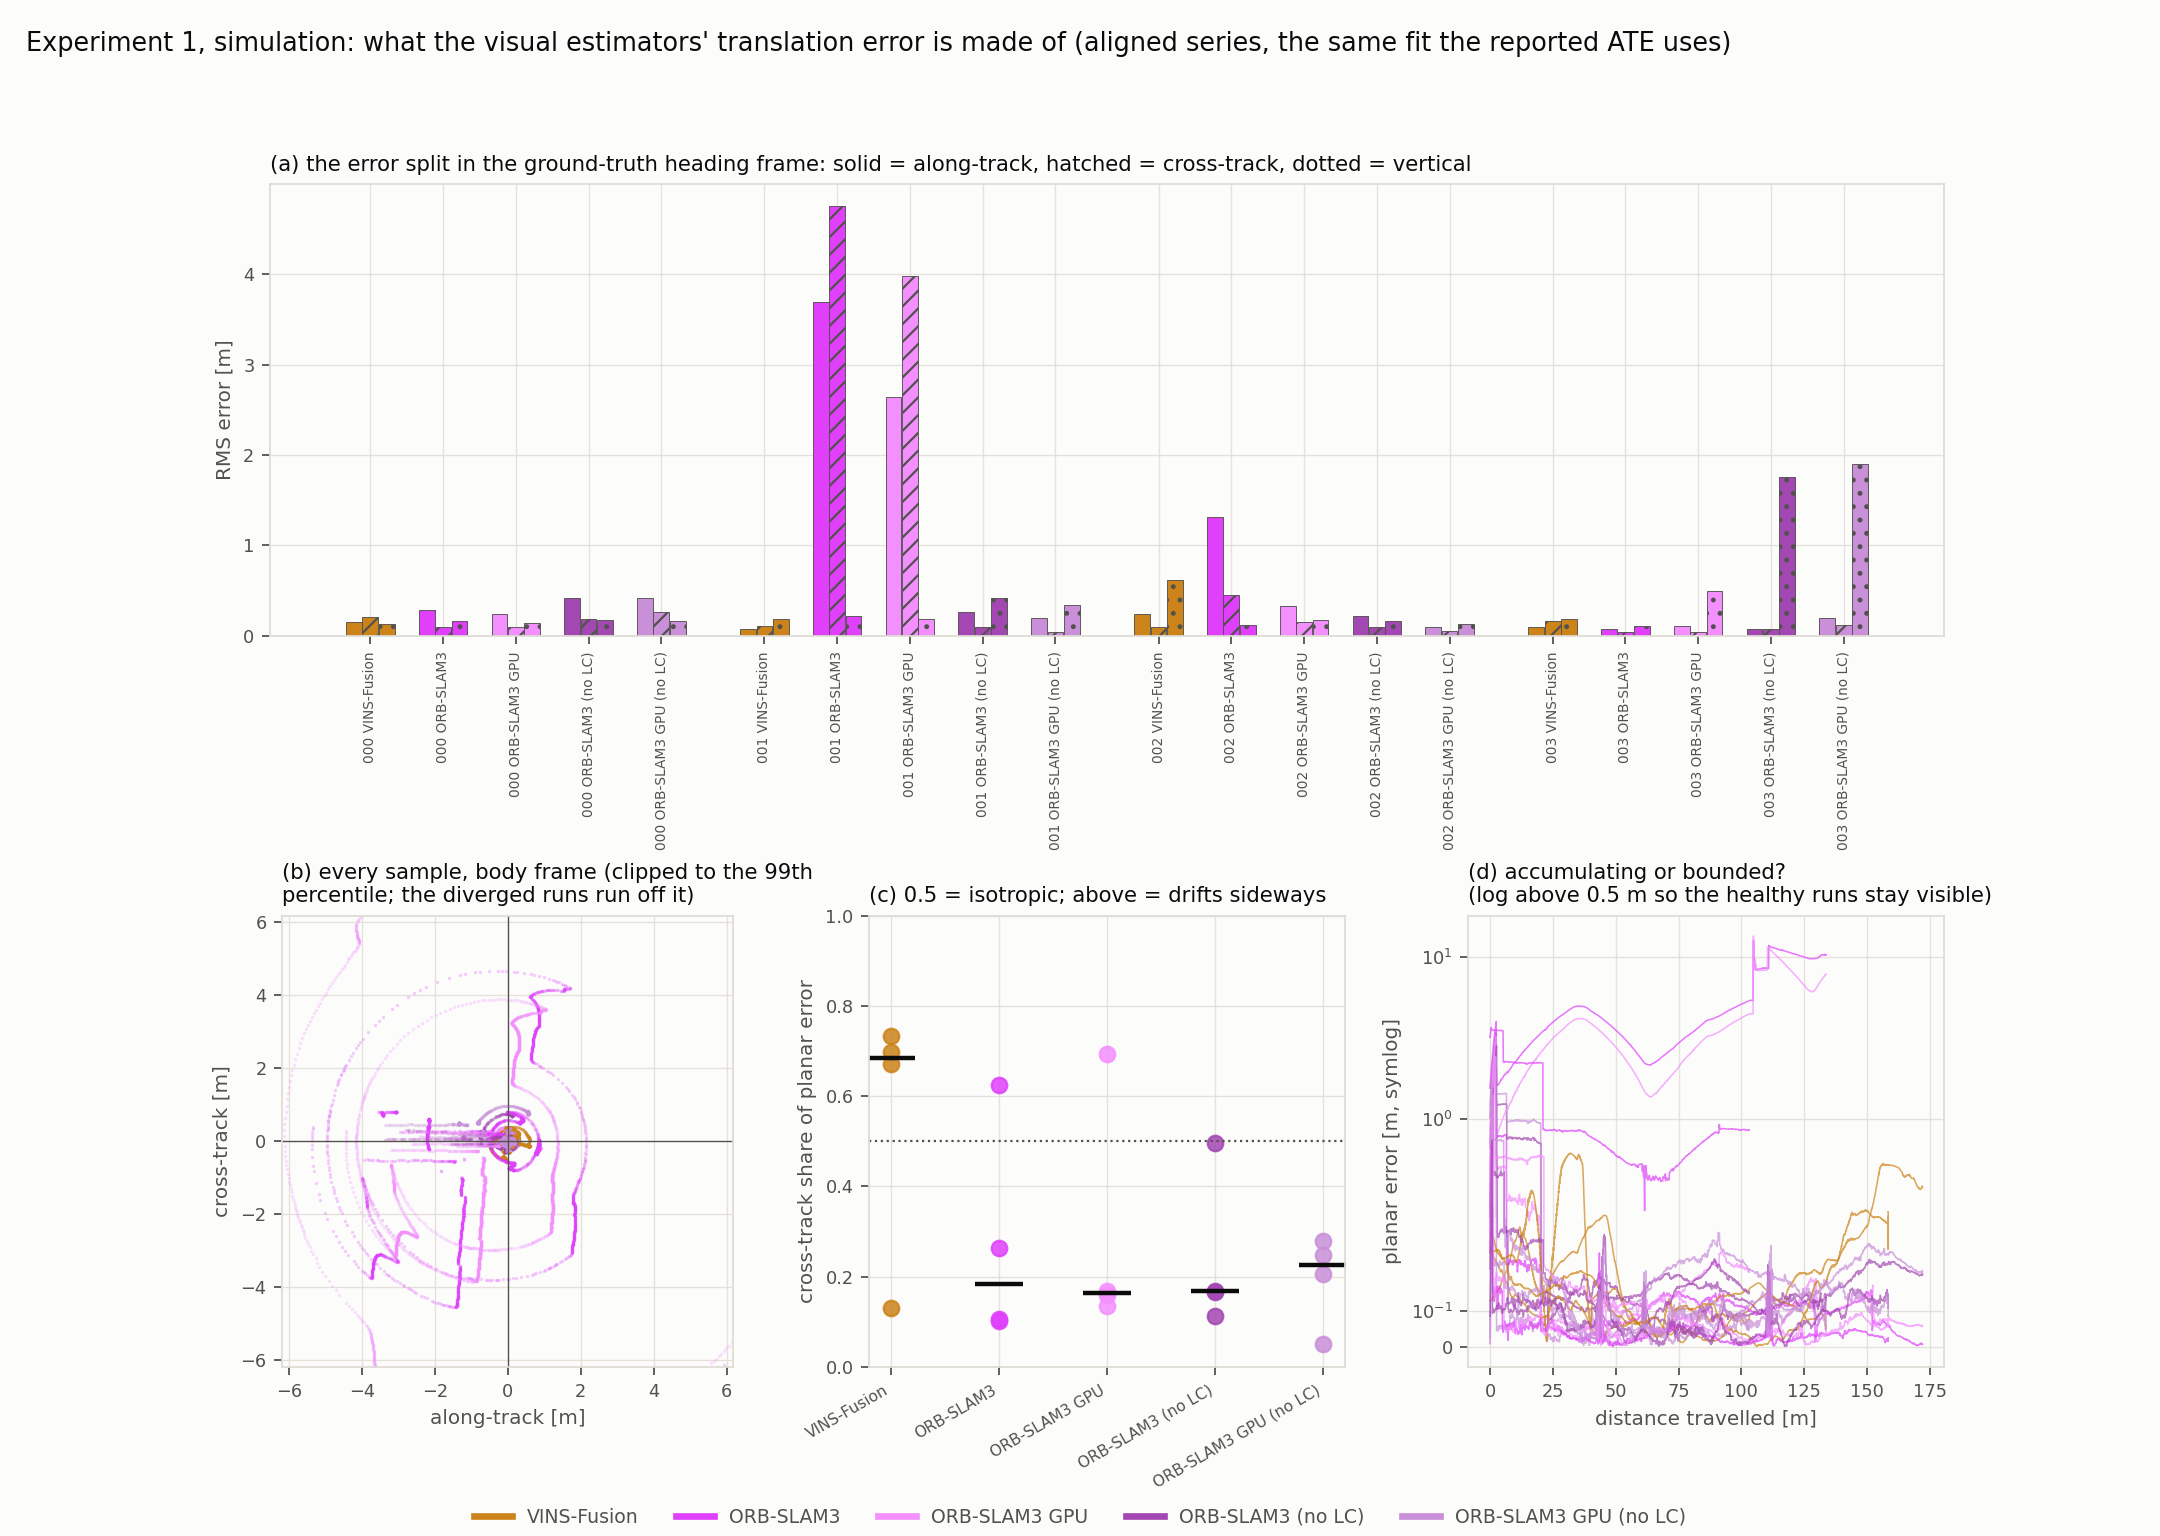
\includegraphics[width=\textwidth]{figures/exp1_translation_pattern.png}
  \caption[What the visual estimators' translation error is made of.]{What the
  translation error is made of, on the aligned series the reported ATE uses.
  (a) the error split per run into along-track, cross-track and vertical;
  (b) every sample in the body frame, clipped to the 99th percentile because
  the five diverged runs reach metres; (c) the cross-track share of the planar
  error, where \num{0.5} is isotropic and above it the estimate drifts
  sideways; (d) error against distance travelled, on a symmetric-log axis above
  \SI{0.5}{\metre} so that the eighteen runs that held tracking stay visible.}
  \label{fig:exp1-translation-pattern}
\end{figure}

\begin{figure}[p]
  \centering
  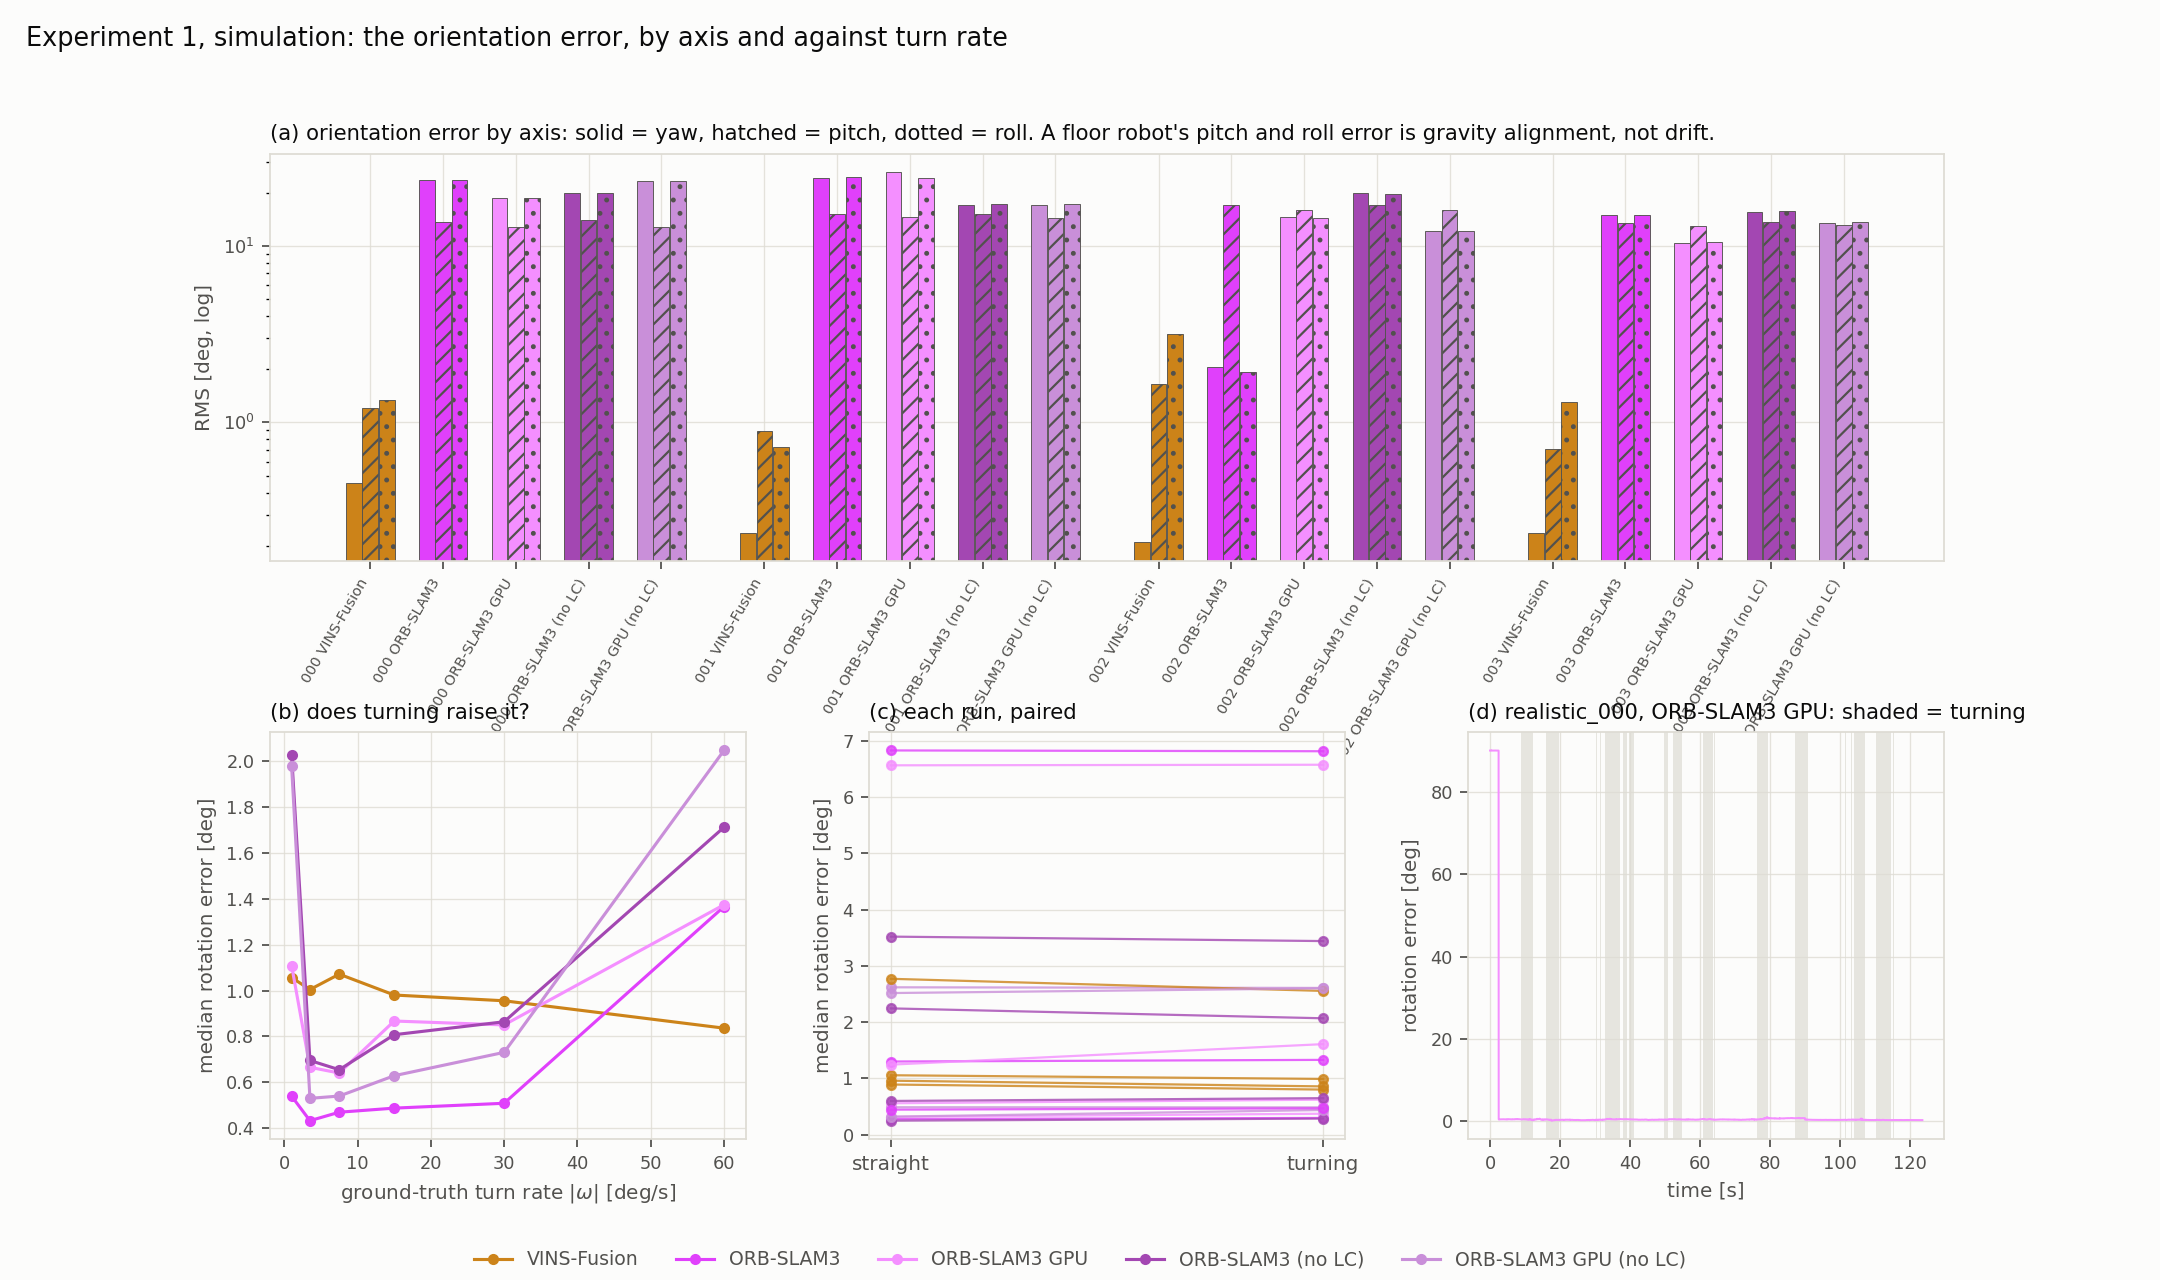
\includegraphics[width=\textwidth]{figures/exp1_rotation_pattern.png}
  \caption[The orientation error by axis and against turn rate.]{The
  orientation error. (a) yaw, pitch and roll RMS per run on a logarithmic axis;
  (b) median rotation error binned by the ground truth's own turn rate;
  (c) the same two medians paired within each run; (d) one run's rotation error
  against time, with the turning segments shaded.}
  \label{fig:exp1-rotation-pattern}
\end{figure}

\paragraph{Latency and resources.} By the design decision of 6 November
2026 the real-time and resource measurement of this experiment is taken only
on the two mapping recordings, each configuration run three times:
\repo{dataset_allsensor_realistic_map} (U layout, \SI{286}{\second}, 8\,725
stereo pairs) and \repo{dataset_allsensor_realistic_01_map} (I layout,
\SI{315}{\second}, 9\,552 pairs). Eighteen runs exist, six configurations of
three repeats each at replay rate 1.0 with no detector: ORB-SLAM3 with the
CPU and with the GPU front end, loop closer disabled, and VINS-Fusion
(\cref{tab:mapping-resources}). The repeats are tight, front-end medians
within \SIrange{1}{7}{\milli\second} of their mean and peak memory within
\SI{30}{\mebi\byte}.

The two pipelines divide the cost differently, and neither is cheaper than
the other outright. VINS-Fusion optimises in \SI{44}{\milli\second} where
ORB-SLAM3's local mapping takes \SIrange{211}{406}{\milli\second}, and holds
its state in a quarter of the memory, but spends more than twice the
processor time: about eight cores of one against three and a half. Their
front ends are within \SI{6}{\milli\second} of each other, and every
configuration keeps \SIrange{75}{96}{\percent} of the bag's frames, so the
choice between them is a memory-against-cores trade, not a speed one.

Between ORB-SLAM3's two front ends the recordings disagree. On the U
recording the GPU extractor behaves as the single runs showed, tracking in
\SI{37}{} against \SI{42}{\milli\second} and keeping \SI{96}{} against
\SI{93}{\percent} of frames; on the I recording the sign reverses, \SI{52}{}
against \SI{44}{\milli\second} and \SI{75}{} against \SI{91}{\percent} kept,
with the local-mapping median at \SI{406}{\milli\second}. VINS-Fusion reads
the same on both recordings (front end \SI{38.1}{} and \SI{38.6}{},
back end \SI{44.3}{} and \SI{44.5}{\milli\second}), so the recordings
themselves do not impose a difference of that size.

\begin{queried}[Confound: run order] The six GPU runs were made consecutively
from 21:04 to 22:04 and the six CPU runs from 23:27 to 00:18, so the
I-recording GPU repeats were the fourth to sixth GPU runs of a session on a
laptop that throttles at \SI{90}{\celsius}; the front-end record notes that
timing comparisons need a cool-start, interleaved order. The six VINS-Fusion
runs are a separate session of 7 November and are not a control for that
state. The U-recording figures are the ones to quote until the I recording is
repeated interleaved. \end{queried} 
% Generated by script/analyse_exp3_rules.py -- do not edit by hand.
\begin{table}[htbp]
\centering
\caption[Real-time and resource measurements on the mapping recordings.]{Real-time and resource measurements on the two mapping recordings, replay rate 1.0, no detector: mean $\pm$ SD over $n$ repeats of each configuration. \textbf{Bold} marks the best mean in each column within a recording. Front-end and back-end are each run's median module latency (ORB-SLAM3: tracking and local mapping; VINS-Fusion: feature tracking and back-end optimisation); throughput is processed frames per second of sensor time; ``Kept'' is the processed fraction of the bag's stereo pairs; CPU is process time over wall time, in percent of one core; RSS the peak resident set. The loop-closer state is read from \repo{loop_closing.csv}.}
\label{tab:mapping-resources}
\scriptsize
\resizebox{\textwidth}{!}{%
\begin{tabular}{lll r rr rrrr}
\toprule
Recording & Estimator & LC & $n$ & Front-end [\si{\milli\second}] & Back-end [\si{\milli\second}] & Throughput [\si{\hertz}] & Kept [\si{\percent}] & CPU [\si{\percent}] & Peak RSS [\si{\mebi\byte}] \\
\midrule
\repo{realistic_map} & ORB-SLAM3 & disabled & 3 & 42.0 $\pm$ 3.3 & 211.3 $\pm$ 14.8 & 28.3 $\pm$ 0.9 & 93 $\pm$ 3 & 379 $\pm$ 11 & 1732 $\pm$ 15 \\
 & ORB-SLAM3 GPU & disabled & 3 & \textbf{36.7 $\pm$ 1.2} & 284.2 $\pm$ 14.7 & \textbf{29.1 $\pm$ 0.4} & \textbf{96 $\pm$ 1} & \textbf{332 $\pm$ 7} & 1794 $\pm$ 19 \\
 & VINS-Fusion & --- & 3 & 38.1 $\pm$ 3.3 & \textbf{44.3 $\pm$ 5.0} & 27.5 $\pm$ 2.7 & 91 $\pm$ 9 & 819 $\pm$ 10 & \textbf{479 $\pm$ 15} \\
\repo{realistic_01_map} & ORB-SLAM3 & disabled & 3 & 43.9 $\pm$ 1.0 & 220.4 $\pm$ 12.6 & \textbf{27.5 $\pm$ 0.3} & \textbf{91 $\pm$ 1} & 381 $\pm$ 6 & 1816 $\pm$ 29 \\
 & ORB-SLAM3 GPU & disabled & 3 & 51.9 $\pm$ 3.8 & 405.7 $\pm$ 22.6 & 22.9 $\pm$ 1.4 & 75 $\pm$ 4 & \textbf{361 $\pm$ 9} & 1719 $\pm$ 21 \\
 & VINS-Fusion & --- & 3 & \textbf{38.6 $\pm$ 0.8} & \textbf{44.5 $\pm$ 1.5} & 27.4 $\pm$ 0.5 & 90 $\pm$ 2 & 814 $\pm$ 5 & \textbf{497 $\pm$ 11} \\
\bottomrule
\end{tabular}}
\end{table}


\paragraph{What each accuracy run cost.} The twenty accuracy runs were
measured for cost as well, on the same machine and in the same sessions, and
\cref{tab:realistic-resources} reports them one row per run. They are not a
substitute for \cref{tab:mapping-resources}: they are single runs on four
short recordings rather than three repeats on two long ones, and the
divergences of \cref{tab:realistic-baseline} are inside them. What they add is
that accuracy and cost can be read on the same runs, which
\cref{fig:realistic-cost-accuracy} draws.

The separation between the two pipelines is the one the mapping recordings
show, at the same sizes. VINS-Fusion holds its state in \SIrange{477}{492}{\mebi\byte}
against ORB-SLAM3's \SIrange{1029}{1350}{\mebi\byte} and optimises in
\SIrange{45}{60}{\milli\second} against \SIrange{189}{286}{\milli\second},
for \SIrange{707}{801}{\percent} of one core against
\SIrange{285}{448}{\percent}. Within ORB-SLAM3 the GPU front end tracks in
\SIrange{29.6}{36.7}{\milli\second} against the CPU front end's
\SIrange{49.2}{54.9}{\milli\second} and draws about a core less, at
\SI{150}{\mebi\byte} more memory. These runs were not interleaved either, so
they carry the same thermal caveat as \cref{tab:mapping-resources} and are
quoted as a second observation of the same separation, not as an independent
one.

The figure's own result is a negative one: no panel shows cost buying
accuracy. Every run that diverged is ORB-SLAM3, and within each front end the
diverged runs cost what the runs that held cost --- with the GPU front end
\SIrange{31.6}{36.7}{\milli\second} against \SIrange{29.6}{36.2}{\milli\second},
overlapping entirely, and with the CPU front end
\SIrange{52.6}{54.9}{\milli\second} against \SIrange{49.2}{51.6}{\milli\second},
a gap of one to five milliseconds across three runs and two recordings, which
one run per cell cannot separate from the recording. A run about to be thrown
several metres by a false loop closure is not working harder beforehand, so no
resource measure on this machine is a usable early warning for the failure
mode this experiment actually found.

% Generated by script/analyse_exp3_rules.py -- do not edit by hand.
\begin{table}[htbp]
\centering
\caption{Realistic world, real-time and resource measurements, one row per run (replay rate 1.0, live detector). Columns as in \cref{tab:extreme-resources}; ``Kept'' here is the processed fraction of the bag's frames, so frames lost before the node's own queue count as lost. Accuracy for the same runs is in \cref{tab:realistic-baseline,tab:realistic-filtered}.}
\label{tab:realistic-resources}
\scriptsize
\resizebox{\textwidth}{!}{%
\begin{tabular}{llllc rr rrrr}
\toprule
Recording & Estimator & Mask & LC & Atlas & Front-end [\si{\milli\second}] & Back-end [\si{\milli\second}] & Throughput [\si{\hertz}] & Kept & CPU [\si{\percent}] & Peak RSS [\si{\mebi\byte}] \\
\midrule
\repo{realistic_000} & ORB-SLAM3 & off & active & no & 57.3 & 313.9 & 18.2 & 60\,\% & 422 & 1167 \\
 & ORB-SLAM3 & off & disabled & no & 49.4 & 260.6 & 21.0 & 69\,\% & 407 & 1205 \\
 & VINS-Fusion & off & --- & no & 50.6 & 63.6 & 17.7 & 58\,\% & 780 & 480 \\
\repo{realistic_001} & ORB-SLAM3 & off & active & no & 63.7 & 321.4 & 17.5 & 58\,\% & 424 & 1101 \\
 & ORB-SLAM3 & off & disabled & no & 59.2 & 311.1 & 18.5 & 59\,\% & 415 & 1094 \\
 & VINS-Fusion & off & --- & no & 47.8 & 62.2 & 20.2 & 67\,\% & 734 & 478 \\
\repo{realistic_002} & ORB-SLAM3 & off & active & no & 59.8 & 308.7 & 20.2 & 67\,\% & 416 & 1182 \\
 & ORB-SLAM3 & off & disabled & no & 58.4 & 300.6 & 20.8 & 69\,\% & 404 & 1060 \\
 & VINS-Fusion & off & --- & no & 47.5 & 61.1 & 22.2 & 73\,\% & 721 & 461 \\
 & ORB-SLAM3+YOLO & class & active & no & 54.3 & 233.0 & 21.2 & 70\,\% & 404 & 1170 \\
 & ORB-SLAM3+YOLO & class & active & yes & 147.7 & 530.1 & 8.4 & 28\,\% & 467 & 1153 \\
 & ORB-SLAM3+YOLO & motion & active & no & 129.6 & 570.7 & 9.6 & 32\,\% & 454 & 1083 \\
 & ORB-SLAM3+YOLO & motion & active & yes & 160.7 & 644.3 & 7.8 & 26\,\% & 462 & 1121 \\
 & ORB-SLAM3+YOLO & class & disabled & no & 97.0 & 426.5 & 13.4 & 44\,\% & 429 & 1028 \\
 & ORB-SLAM3+YOLO & class & disabled & yes & 58.9 & 261.2 & 18.8 & 62\,\% & 385 & 1204 \\
 & ORB-SLAM3+YOLO & motion & disabled & no & 106.6 & 511.0 & 11.6 & 38\,\% & 435 & 1008 \\
 & ORB-SLAM3+YOLO & motion & disabled & yes & 135.6 & 545.9 & 8.9 & 29\,\% & 443 & 1136 \\
 & VINS-Fusion+YOLO & class & --- & no & 63.6 & 85.3 & 17.1 & 56\,\% & 718 & 485 \\
 & VINS-Fusion+YOLO & motion & --- & no & 86.3 & 103.5 & 12.9 & 43\,\% & 701 & 489 \\
\repo{realistic_003} & ORB-SLAM3 & off & active & no & 54.2 & 292.5 & 24.8 & 81\,\% & 398 & 1190 \\
 & ORB-SLAM3 & off & disabled & no & 62.0 & 323.5 & 22.0 & 73\,\% & 402 & 1182 \\
 & VINS-Fusion & off & --- & no & 48.2 & 63.7 & 25.0 & 82\,\% & 709 & 494 \\
 & ORB-SLAM3+YOLO & class & active & no & 59.6 & 253.6 & 20.9 & 69\,\% & 409 & 1197 \\
 & ORB-SLAM3+YOLO & class & active & yes & 126.6 & 480.0 & 10.6 & 35\,\% & 459 & 1243 \\
 & ORB-SLAM3+YOLO & motion & active & no & 114.2 & 478.0 & 12.3 & 41\,\% & 434 & 1145 \\
 & ORB-SLAM3+YOLO & motion & active & yes & 214.9 & 745.0 & 6.7 & 22\,\% & 446 & 1164 \\
 & ORB-SLAM3+YOLO & motion & active & yes & 164.9 & 654.0 & 8.7 & 29\,\% & 442 & 1223 \\
 & ORB-SLAM3+YOLO & class & disabled & no & 92.0 & 271.4 & 15.1 & 50\,\% & 424 & 1220 \\
 & ORB-SLAM3+YOLO & class & disabled & yes & 77.8 & 321.4 & 17.1 & 56\,\% & 411 & 1307 \\
 & ORB-SLAM3+YOLO & motion & disabled & no & 93.3 & 450.1 & 15.0 & 49\,\% & 415 & 1133 \\
 & VINS-Fusion+YOLO & class & --- & no & 94.3 & 107.3 & 13.0 & 43\,\% & 673 & 471 \\
 & VINS-Fusion+YOLO & motion & --- & no & 77.8 & 100.7 & 15.6 & 51\,\% & 736 & 486 \\
\bottomrule
\end{tabular}}
\end{table}


\begin{figure}[htbp]
  \centering
  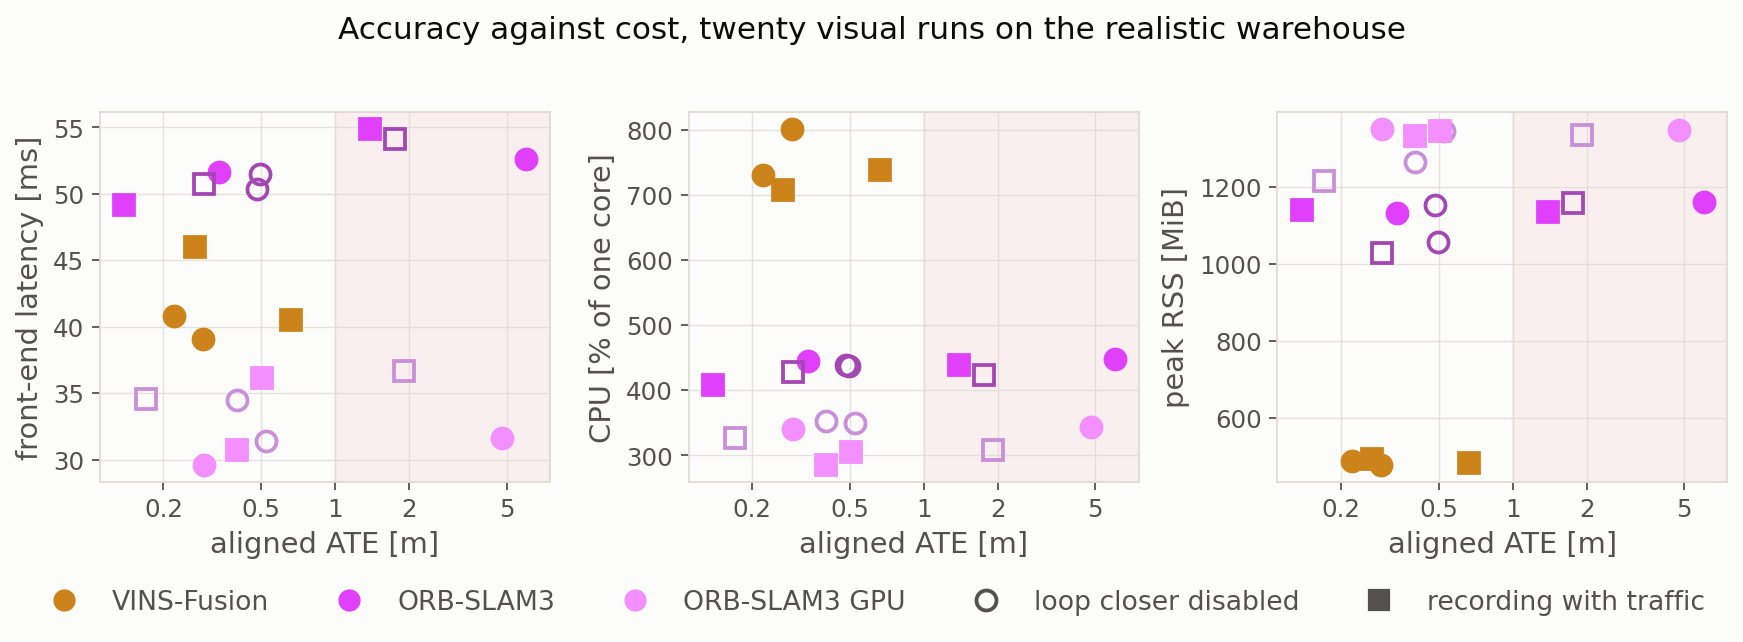
\includegraphics[width=\textwidth]{figures/realistic_cost_accuracy.png}
  \caption[Accuracy against cost on the twenty realistic-world runs.]{Accuracy
  against cost, one point per visual run on the four realistic-warehouse
  recordings, from \cref{tab:realistic-baseline,tab:realistic-resources}.
  Aligned ATE is on a logarithmic axis in all three panels; the shaded band is
  the region above \SI{1}{\metre}, which holds the five diverged runs. Orange
  is VINS-Fusion, magenta ORB-SLAM3 with the CPU front end and light magenta
  with the GPU front end; an open marker is a run with the loop closer
  disabled and a square a recording carrying traffic. Cost is the run's median
  front-end latency, its process time as a percentage of one core, and its
  peak resident set.}
  \label{fig:realistic-cost-accuracy}
\end{figure}



\paragraph{How repeatable is any of this?} The eighteen runs above are the only
repeated runs in the simulation campaign, and scoring them for accuracy as well
as for time measures something no other result in this chapter can:
how much an estimate moves when nothing changes.
\Cref{tab:mapping-repeats} gives the spread over the three repeats of each
configuration. The two estimators answer differently. VINS-Fusion repeats to
\SI{0.094}{\metre} on the U recording and \SI{0.035}{} on the I, five and
seven per cent of its own mean. ORB-SLAM3 does not: its three repeats span
\SI{0.089}{\metre} on the U recording and \SI{0.277}{} on the I with the CPU
front end, and \SI{0.016}{} and \SI{0.236}{\metre} with the GPU front end ---
on the I recording that is half to four fifths of the configuration's own mean,
from the same binary, the same configuration file and the same bag, with the
loop closer disabled in all six.

The frame counts in the same table are consistent with why. VINS-Fusion
processed every frame of both recordings in all six runs, so it saw identical
input each time; ORB-SLAM3 kept \SIrange{90}{97}{\percent} with the CPU front
end and \SIrange{70}{98}{\percent} with the GPU one, and which frames a run
loses depends on how the laptop was scheduling at that moment. That is a
consistent explanation and not a demonstrated one: a keyframe-based system with
a bundle adjustment on its own thread need not be deterministic even on
identical input. Separating the two would need a run at a replay rate slow
enough to drop nothing, which this chapter does not have. The worst spread also
belongs to the I recording, whose repeats carry the thermal confound noted
above, so part of \SI{0.277}{\metre} may be the laptop rather than the
estimator.

Read against \cref{tab:realistic-baseline} this sets a floor under what that
table can be asked. A difference of less than about a quarter of a metre
between two ORB-SLAM3 arms is inside the spread measured here and should not be
read as an effect; this is the quantity the bold marking of that table was
hedged against, now measured. Two of the chapter's findings survive it and one
is strengthened. The five divergences are \SIrange{1.39}{6.02}{\metre}, five to
twenty times the floor, and the false closure that causes the largest of them
is reproduced by both front ends on the same frame. The claim that the front
end changes throughput and not accuracy is supported rather than weakened:
the CPU and GPU arms differ by less than this floor on every recording, which
is what having no effect looks like. What should not be carried further is any
ordering of two ORB-SLAM3 arms that rests on a gap smaller than it.

% Generated by script/analyse_mapping_repeats.py -- do not edit by hand.
\begin{table}[htbp]
\centering
\caption[Run-to-run spread over the three repeats of each mapping-recording configuration.]{Run-to-run spread over the three repeats of each configuration on the two mapping recordings, the only repeated runs in the simulation campaign; the same eighteen runs as \cref{tab:mapping-resources}, scored for accuracy. Every run has its loop closer disabled, read from \repo{loop_closing.csv}. ``ATE'' is mean $\pm$ SD over the three repeats and ``spread'' the largest difference between two of them; ``Max'' is the largest error after the initialisation transient, on the convention of the accuracy table of \cref{sec:exp1-sim}. The three repeats of a configuration were run back to back rather than interleaved, so a drift across them is confounded with the laptop's thermal state (\cref{sec:exp1-sim}); the Kept column is where that would show.}
\label{tab:mapping-repeats}
\small
\resizebox{\textwidth}{!}{%
\begin{tabular}{llr rrrrr}
\toprule
Recording & Estimator & $n$ & ATE [\si{\metre}] & spread [\si{\metre}] & Max [\si{\metre}] & ATE/path [\si{\percent}] & Kept \\
\midrule
\repo{realistic_map} & ORB-SLAM3 & 3 & 0.189 $\pm$ 0.045 & 0.089 & 0.748 $\pm$ 0.267 & 0.05 $\pm$ 0.01 & 0.94 $\pm$ 0.03 \\
 & ORB-SLAM3 GPU & 3 & 0.144 $\pm$ 0.008 & 0.016 & 0.345 $\pm$ 0.033 & 0.04 $\pm$ 0.00 & 0.96 $\pm$ 0.01 \\
 & VINS-Fusion & 3 & 1.915 $\pm$ 0.049 & 0.094 & 3.617 $\pm$ 0.239 & 0.51 $\pm$ 0.01 & 1.00 $\pm$ 0.00 \\
\addlinespace
\repo{realistic_01_map} & ORB-SLAM3 & 3 & 0.348 $\pm$ 0.149 & 0.277 & 1.517 $\pm$ 0.749 & 0.09 $\pm$ 0.04 & 0.91 $\pm$ 0.01 \\
 & ORB-SLAM3 GPU & 3 & 0.433 $\pm$ 0.118 & 0.236 & 2.691 $\pm$ 0.338 & 0.11 $\pm$ 0.03 & 0.76 $\pm$ 0.04 \\
 & VINS-Fusion & 3 & 0.491 $\pm$ 0.017 & 0.035 & 5.088 $\pm$ 0.167 & 0.13 $\pm$ 0.00 & 1.00 $\pm$ 0.00 \\
\bottomrule
\end{tabular}}
\end{table}


\paragraph{Limitations, each stated once.} \emph{$n$:} one run per cell on the
four accuracy recordings, in both families; the three repeats of each
mapping-recording configuration (\cref{tab:mapping-repeats}) are the only
within-configuration spread the campaign measures, and they are on different
routes. \emph{Equal handicap, not equal effort:} the shared inertial model
was fitted to neither family. \emph{Idealised wheels:} simulated encoders
with slip under \SI{1}{\percent}, the proprioceptive estimators' best case.
\emph{Route and traffic confounded:} no two recordings share a route, so
traffic is a condition of a recording and not a tested factor.
\emph{Three-dimensional ATE:} the metric charges vertical drift to a floor
robot; the planar onset table is the complement, not a replacement.
\emph{Deployment rate on one laptop:} frame retention and every latency
figure are properties of this machine at rate 1.0, and the mapping-bag
repeats were not interleaved between front ends. \emph{Run bookkeeping:} one
directory held a run on another recording for a day; the manifest caught it,
and the launch should refuse an output directory whose name disagrees with
its dataset.

\begin{queried}[Resolved: \repo{realistic_002/loopclosing_gpu}]
Earlier on 6 November this run was reported as closure-free from its
\repo{loop_closing.csv} and queried. Its manifest shows the real cause: it was
launched on the \repo{realistic_003} bag with \repo{realistic_002}'s output
path, so it was scored against the wrong truth (\SI{4.94}{\metre},
\SI{48.9}{\degree}, 139\,\% of the recording's frames processed). It is set
aside, not deleted; the configuration was re-run on the right bag the same
evening and every table here carries that run.
\end{queried}

\begin{queried}[Open: the false closure is diagnosed from its correction, not from the images]
The \SI{14}{\metre} correction and the one-aisle keyframe separation identify
the \repo{realistic_001} closure as false, and both front ends agree; the
matched image pair has not been inspected, and the two April-style guards
that would catch it (a covisibility-consistency window, or a maximum
correction against the inertial drift bound) are untested. Until one is, the
finding is a diagnosis, not a fix.
\end{queried}

\paragraph{Summary.} Two families were scored on the same four recordings.
Among the non-visual estimators IMU-only dead reckoning drifts by
\SIrange{12}{23}{\metre} and wheel odometry by \SIrange{1.0}{4.8}{\metre} of
aligned ATE; the EKF, run on the visual systems' own inertial noise as the
design requires, holds \SIrange{0.68}{2.80}{\metre}, while the same filter on
a measured noise model would hold \SIrange{0.21}{0.58}{\metre}. Among the
visual ones VINS-Fusion holds \SIrange{0.22}{0.66}{\metre} with no jump and
is worst on the U layout with traffic; ORB-SLAM3 holds
\SIrange{0.14}{0.52}{\metre} in eleven runs of sixteen, and its five
divergences are the loop closer's: a false closure on the I layout's repeated
aisles that puts both front ends \SIrange{4.8}{6.0}{\metre} off, a vertical
drift on the same layout with traffic that only the closer corrects, and one
initialisation offset. Neither pipeline loses tracking on any recording, with
or without traffic, and the front end changes throughput
(\SIrange{97}{99}{\percent} of frames kept against \SIrange{72}{94}{\percent})
and not accuracy. Across the families the EKF at the shared handicap loses to
VINS-Fusion on every recording and the measured-noise diagnostic beats it on
three of four, so on these routes the noise model is worth more than the
choice of estimator. Against the project's target of \SI{0.05}{\metre} ATE no
estimator qualifies; against the \SI{1.5}{\metre} RPE bound at
\SI{1}{\second}, all but the IMU do. On cost, VINS-Fusion optimises five to
nine times faster than ORB-SLAM3's local mapping and in a quarter of the
memory, for more than twice the processor time.

\paragraph{Future plan.} Fit the visual systems' inertial noise to this
platform rather than copying a file, since the slot shows the noise model is
worth more than the estimator; feed the VIO pose into the EKF as a third
measurement; add a correction bound to the loop closer and test it on
\repo{realistic_001}; repeat the mapping-recording runs interleaved between
all three configurations from a cool start, so that the thermal state is
shared rather than confounded with the configuration; and record a second
route in each layout so that traffic and route are separable.

\FloatBarrier

\FloatBarrier
\subsection{Real robot}
\label{sec:exp1-real}

\slotstatus{partial}{Four real recordings with an independent planar reference
(\repo{dataset_realv6_000}, \repo{dataset_realv7_000} to \repo{_002}). A
non-visual baseline exists: wheel+gyro dead reckoning with the feedback speed
scaled by a factor fitted once against the tracker on \repo{realv7_000} and
held on the other three. The visual arm is ORB-SLAM3 in four configurations on
each recording, sixteen runs, all made with the fork's patch-15
initialisation switches and scored with no repair applied; they give
\SIrange{0.404}{0.480}{\metre} on \repo{realv6_000},
\SIrange{0.251}{0.268}{} on \repo{realv7_000}, \SIrange{0.442}{1.278}{} on
\repo{_001} and \SIrange{0.172}{0.198}{} on \repo{_002}. Across the held
recordings the two families are in the same accuracy class, the baseline
leading on one, tying on one and losing the third. The EKF of the simulation
slot cannot be formed, because the rig publishes no steering measurement;
VINS-Fusion has no valid run on any recording; and every value is provisional
until the marker-to-IMU lever arm is measured.}

\textbf{Objective.} The real-robot half of the simulation question: do the
visual pipelines track the robot against an independent reference, and does a
non-visual estimator match them on the same recordings.

\textbf{Process.} Two groups of runs share these recordings.


\emph{Non-visual.} The bags carry \repo{/feedback/velocity} and
\repo{/feedback/steering} (\SI{50}{\hertz}, \texttt{std\_msgs/Float64}) and
the WitMotion yaw sensor on \repo{/hwt101ct_yaw_publisher} (\SI{200}{\hertz}).
The velocity is in a firmware unit, not metres per second; the steering is a
command echo that takes two values (0 and $-30$) on every recording and so
carries no yaw rate; the yaw sensor's orientation field is identity and its
rate on the $y$ axis is the live gyro (the sensor is mounted with $y$
vertical: that axis integrates to \SI{6.29}{rad} over \repo{realv7_000}, whose
tracker heading sweeps \SI{6.3}{rad}; $x$ and $z$ integrate to under
\SI{0.05}{rad}).

\repo{script/real_wheel_baseline.py} integrates heading from
that gyro with its rest bias removed (\SIrange{3}{7}{\second} at rest at the
head of each bag) and position from the scaled speed. The scale $k$, the gyro
axis and its sign are fitted on \repo{realv7_000} alone by minimising the
planar ATE after rigid $SE(2)$ alignment with scale fixed (a wrong sign
mirrors the path, which a proper rotation cannot align), then held: the fit
recording's own score is a calibration, the three held scores are the result.
The fitted $k=0.325$ agrees with the plain path-length ratio of each
\repo{realv7} bag (0.323 to 0.329). The time offset between tracker and bag is
the wheel-speed cross-correlation of \repo{script/eval_real_gt.py}
($r=0.93$ to $0.99$ on \repo{realv7}, $0.61$ on the sparse \repo{realv6}
export), scoring is that script's planar procedure at the tracker's own
samples, and the one off-path \repo{realv6} sample is removed by the rule the
realv6 analysis fixed.

The rig's wheelbase, \SI{0.60}{\metre}, is recorded
and unused: with no steering measurement there is nothing to put through a
bicycle model, so the yaw-rate observation that gives the simulation EKF its
bias state does not exist, and that filter would reduce to this integration.


\emph{Visual.} The bag was replayed into each node at real time on the
afternoon of 3 November 2026; no detector ran. ORB-SLAM3 used
\repo{config/wil/stereo_imu.yaml} with the repaired library (fork patches
11--14b, node and library built alike), the 3 November stereo extrinsic and
\texttt{IMU.NoiseGyro} 0.1 with \texttt{IMU.NoiseAcc} 1.0, ten times the values
that had been copied from the VINS file, in four configurations: GPU or CPU
feature extractor, loop closing on or off. VINS-Fusion used the same file with
the gravity norm of an August recording. Earlier runs on this bag were
overwritten by these and are not reported. The optical tracker export was scored
with the real-robot procedure of Experiment~1.

\textbf{Dataset.} \SI{220}{\second}, 6\,601 stereo pairs at \SI{30}{\hertz},
RealSense IMU at \SI{200}{\hertz} on the inherited topic name, wheel-speed
feedback, a figure-of-eight of about \SI{27}{\metre} at a median
\SI{0.15}{\metre\per\second} on the Gensurv floor, no scripted moving objects.
Tracker export: 277 samples, median spacing \SI{0.6}{\second}, 66 gaps above
\SI{1}{\second}, one sample \SI{5.2}{\metre} off the path at \SI{184.9}{\second}.

\textbf{Datasets.} The four real recordings that carry an independent
planar reference: routes of \SIrange{22}{37}{\metre} over
\SIrange{97}{219}{\second}. Sources:
\path{output/compare/real/exp1-wheel/} (\repo{wheel_metrics.csv},
\repo{manifest.json}), estimates under \path{output/output_wheel/real/}.

\paragraph{Reporting rules, visual arms.} \path{script/eval_real_gt.py}: rigid SE(2)
alignment with scale fixed, lever arm set to zero and unmeasured, every value
provisional. The export fails the tool's gap and step rules, so the tool labels
each run \emph{failed (ground truth invalid)}; the values below are diagnostics.
All are scored with the one off-path sample removed, an edit recorded here and
applied nowhere else; \cref{tab:realv6-cleaning} shows what that sample does to
one run. The bag was not on the machine, so the time offset is pinned to the
value the wheel-speed cross-correlation found on 2 November and the manifests
record the substitution. Sources: \path{output/compare/real/realv6_1103pm_*/},
\path{output/compare/real/realv6-insights/}, run directories under
\path{output/output_orb/real/dataset_realv6_000/} and
\path{output/output_vins/real/dataset_realv6_000/}.

\subsubsection{Non-visual baseline}

\paragraph{Results.} \Cref{tab:exp1-real-wheel} and \cref{fig:exp1-real-wheel}.
On the fit recording the baseline reads \SI{0.06}{\metre} ATE with a path ratio
of 0.99, which is the calibration. Held, it reads \SI{0.26}{} and
\SI{0.22}{\metre} on \repo{realv7_001} and \repo{_002} with path ratios of
0.99 and 1.01, and \SI{0.46}{\metre} on \repo{realv6_000} against its sparse
export, with no jump and a relative error at \SI{1}{\second} of
\SIrange{0.01}{0.02}{\metre}.

% Generated by script/real_wheel_baseline.py -- do not edit by hand.
\begin{table}[htbp]
\centering
\caption[Wheel+gyro dead reckoning against the optical tracker.]{Wheel+gyro dead reckoning on the real recordings against the optical tracker: the feedback speed scaled by $k$ (fitted on \repo{realv7_000} by minimising planar ATE, held on the others), heading from the integrated gyro with its rest bias removed, rigid $SE(2)$ alignment with scale fixed, lever arm zero and unmeasured. ATE at the tracker's samples; path ratio is estimated over true path length.}
\label{tab:exp1-real-wheel}
\small
\resizebox{\textwidth}{!}{%
\begin{tabular}{llrrrrrrr}
\toprule
Recording & Role & $k$ & Offset [\si{\second}] ($r$) & Samples & ATE RMSE [\si{\metre}] & ATE max [\si{\metre}] & Path ratio & RPE$_{1\,\mathrm{s}}$ [\si{\metre}] \\
\midrule
\repo{realv7_000} & fit & 0.325 & -2.57 (0.99) & 491 & 0.057 & 0.11 & 0.990 & 0.008 \\
\repo{realv7_001} & held & 0.325 & -3.77 (0.98) & 632 & 0.259 & 0.47 & 0.988 & 0.021 \\
\repo{realv7_002} & held & 0.325 & -2.60 (0.93) & 499 & 0.219 & 0.27 & 1.006 & 0.008 \\
\repo{realv6_000} & held & 0.325 & -4.14 (0.61) & 233 & 0.463 & 0.70 & 1.041 & 0.015 \\
\bottomrule
\end{tabular}}
\end{table}


\begin{figure}[htbp]
  \centering
  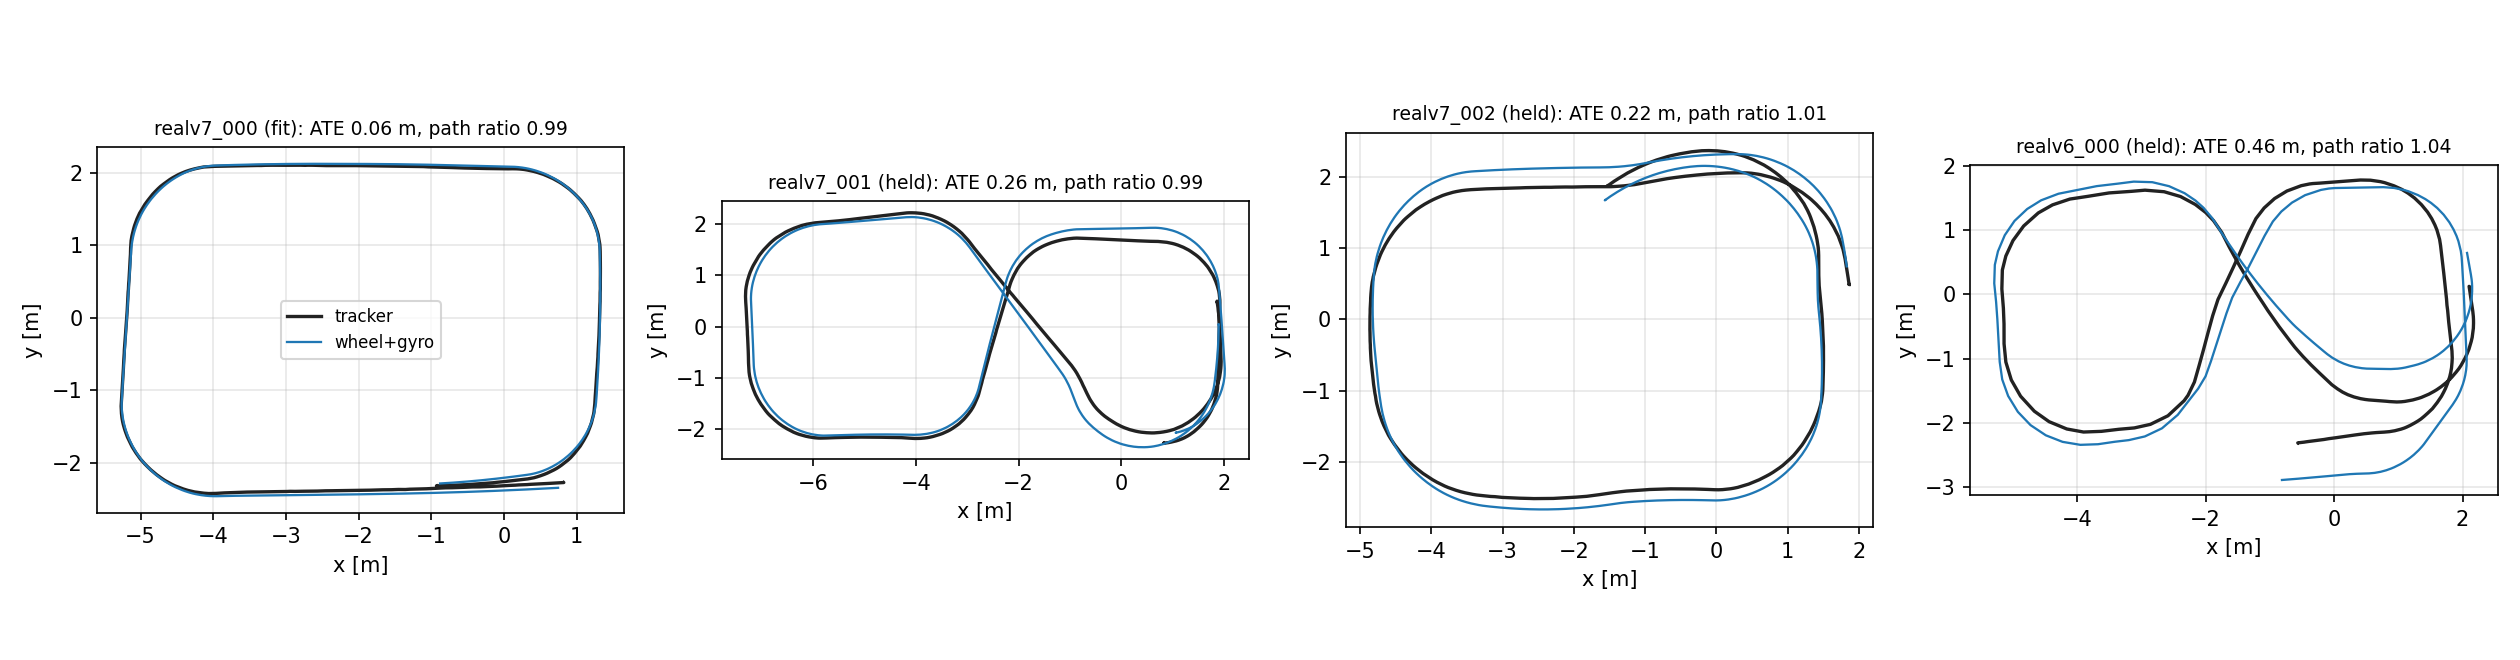
\includegraphics[width=\textwidth]{../../../output/compare/real/exp1-wheel/wheel_paths_light.png}
  \caption[Wheel+gyro dead reckoning against the tracker.]{Wheel+gyro dead
  reckoning (blue) against the tracker (black) after
  rigid planar alignment, one panel per recording; the first is the recording
  the speed scale was fitted on.}
  \label{fig:exp1-real-wheel}
\end{figure}

\paragraph{Analysis.} The comparison this slot exists for now has a number on
both sides, and it does not favour vision. On the same recordings the best
ORB-SLAM3 configuration reads \SI{0.44}{\metre} on \repo{realv7_001},
\SI{0.47}{\metre} on \repo{realv7_002} and \SI{0.46}{\metre} on
\repo{realv6_000} (the real-robot section below, after the scorer's frame
repair); the scaled dead reckoning reads \SI{0.26}{}, \SI{0.22}{} and
\SI{0.46}{\metre}, with path ratios within \SI{4}{\percent} of one where the
visual runs read \SIrange{5}{15}{\percent} long.

Three things bound that reading. The scale is a fitted constant, not a measured one, so the baseline
has had one parameter tuned against the truth it is scored on, on a different
recording; a second calibration route, the wheel circumference and the gear
ratio, would remove that. The routes are \SIrange{22}{37}{\metre} with the
robot at \SI{0.2}{\metre\per\second}: a gyro drifting at the measured rest
bias of \SIrange{0.003}{0.006}{\radian\per\second} accumulates
\SIrange{0.3}{1.3}{\radian} over a run if the bias is not removed and under
\SI{0.1}{\radian} after the rest-window removal, and on a longer route that
term grows while the visual error need not. And the lever arm is zero for
both sides. Against the project's targets no run approaches \SI{0.05}{\metre}
except the calibration itself; every run is inside the \SI{1.5}{\metre} RPE
bound.

\begin{queried}[Open: the realv6 scale]
On \repo{realv6_000} the path-length ratio gives $k=0.43$ where the three
\repo{realv7} bags give $0.32$ to $0.33$, yet the held $k=0.325$ scores a path
ratio of 1.04 on the matched samples. The export is at \SI{1.7}{\hertz} and
fails the validity rules, and the recording predates \repo{realv7} by three
days; whether the firmware unit changed or the sparse export misstates the
path length is not decided, and the \repo{realv6} row is a diagnostic.
\end{queried}

\subsubsection{Visual estimators}

\paragraph{Results.} ORB-SLAM3 follows the whole \SI{218}{\second} route in
every configuration: \SI{0.52}{} and \SI{0.46}{\metre} with the GPU extractor
(loop closing on and off), \SI{0.62}{} and \SI{1.03}{\metre} with the CPU
extractor, which drops two thirds of the frames at real time
(\cref{tab:realv6-final}, \cref{fig:realv6-paths}). VINS-Fusion tracked
\SI{18}{\second} before 217 IMU-gap resets took over (\cref{tab:realv6-vins})
and has no entry in the accuracy table.

\begin{table}[htbp]
\centering
\scriptsize\setlength{\tabcolsep}{3pt}
\caption[Realv6: every surviving run against the cleaned tracker truth.]{ORB-SLAM3 on \repo{dataset_realv6_000} against the cleaned tracker truth, 3 November 2026 afternoon series: repaired library, replay rate 1.0, 3 November stereo extrinsic, \texttt{IMU.NoiseGyro} 0.1 and \texttt{IMU.NoiseAcc} 1.0, GPU or CPU feature extractor, loop closing (LC) on or off. Aligned planar ATE after a rigid SE(2) fit with scale fixed; RPE at \SI{1}{\second} translational; path ratio = estimate / truth; resets = \repo{local_mapping_bad_imu} map resets; dropped = camera frames the node's queue discarded of about 6\,480 received. Lever arm tracker-marker to IMU unmeasured (zero applied); time offset pinned to \SI{-4.14}{\second}; all values provisional under the scorer's validity rules. \\textbf{Bold} marks the lowest ATE of the five runs; with one run per configuration that records which run came lowest, not that the configuration is better.}
\label{tab:realv6-final}
\begin{tabular}{lrrrrrrr}
\toprule
Run & ATE [m] & median [m] & max [m] & RPE$_{1\,\mathrm{s}}$ [m] & path ratio & resets & dropped \\
\midrule
ORB-SLAM3, GPU, LC on & 0.52 & 0.44 & 1.11 & 0.057 & 0.85 & 2 & 2420 \\
ORB-SLAM3, CPU, LC on & 0.62 & 0.48 & 1.38 & 0.110 & 0.88 & 2 & 4363 \\
ORB-SLAM3, GPU, LC off & \textbf{0.46} & 0.36 & 0.99 & 0.056 & 0.87 & 0 & 3201 \\
ORB-SLAM3, CPU, LC off & 1.03 & 0.89 & 1.83 & 0.223 & 0.96 & 3 & 4204 \\
\bottomrule
\end{tabular}
\end{table}


\begin{figure}[p]
  \centering
  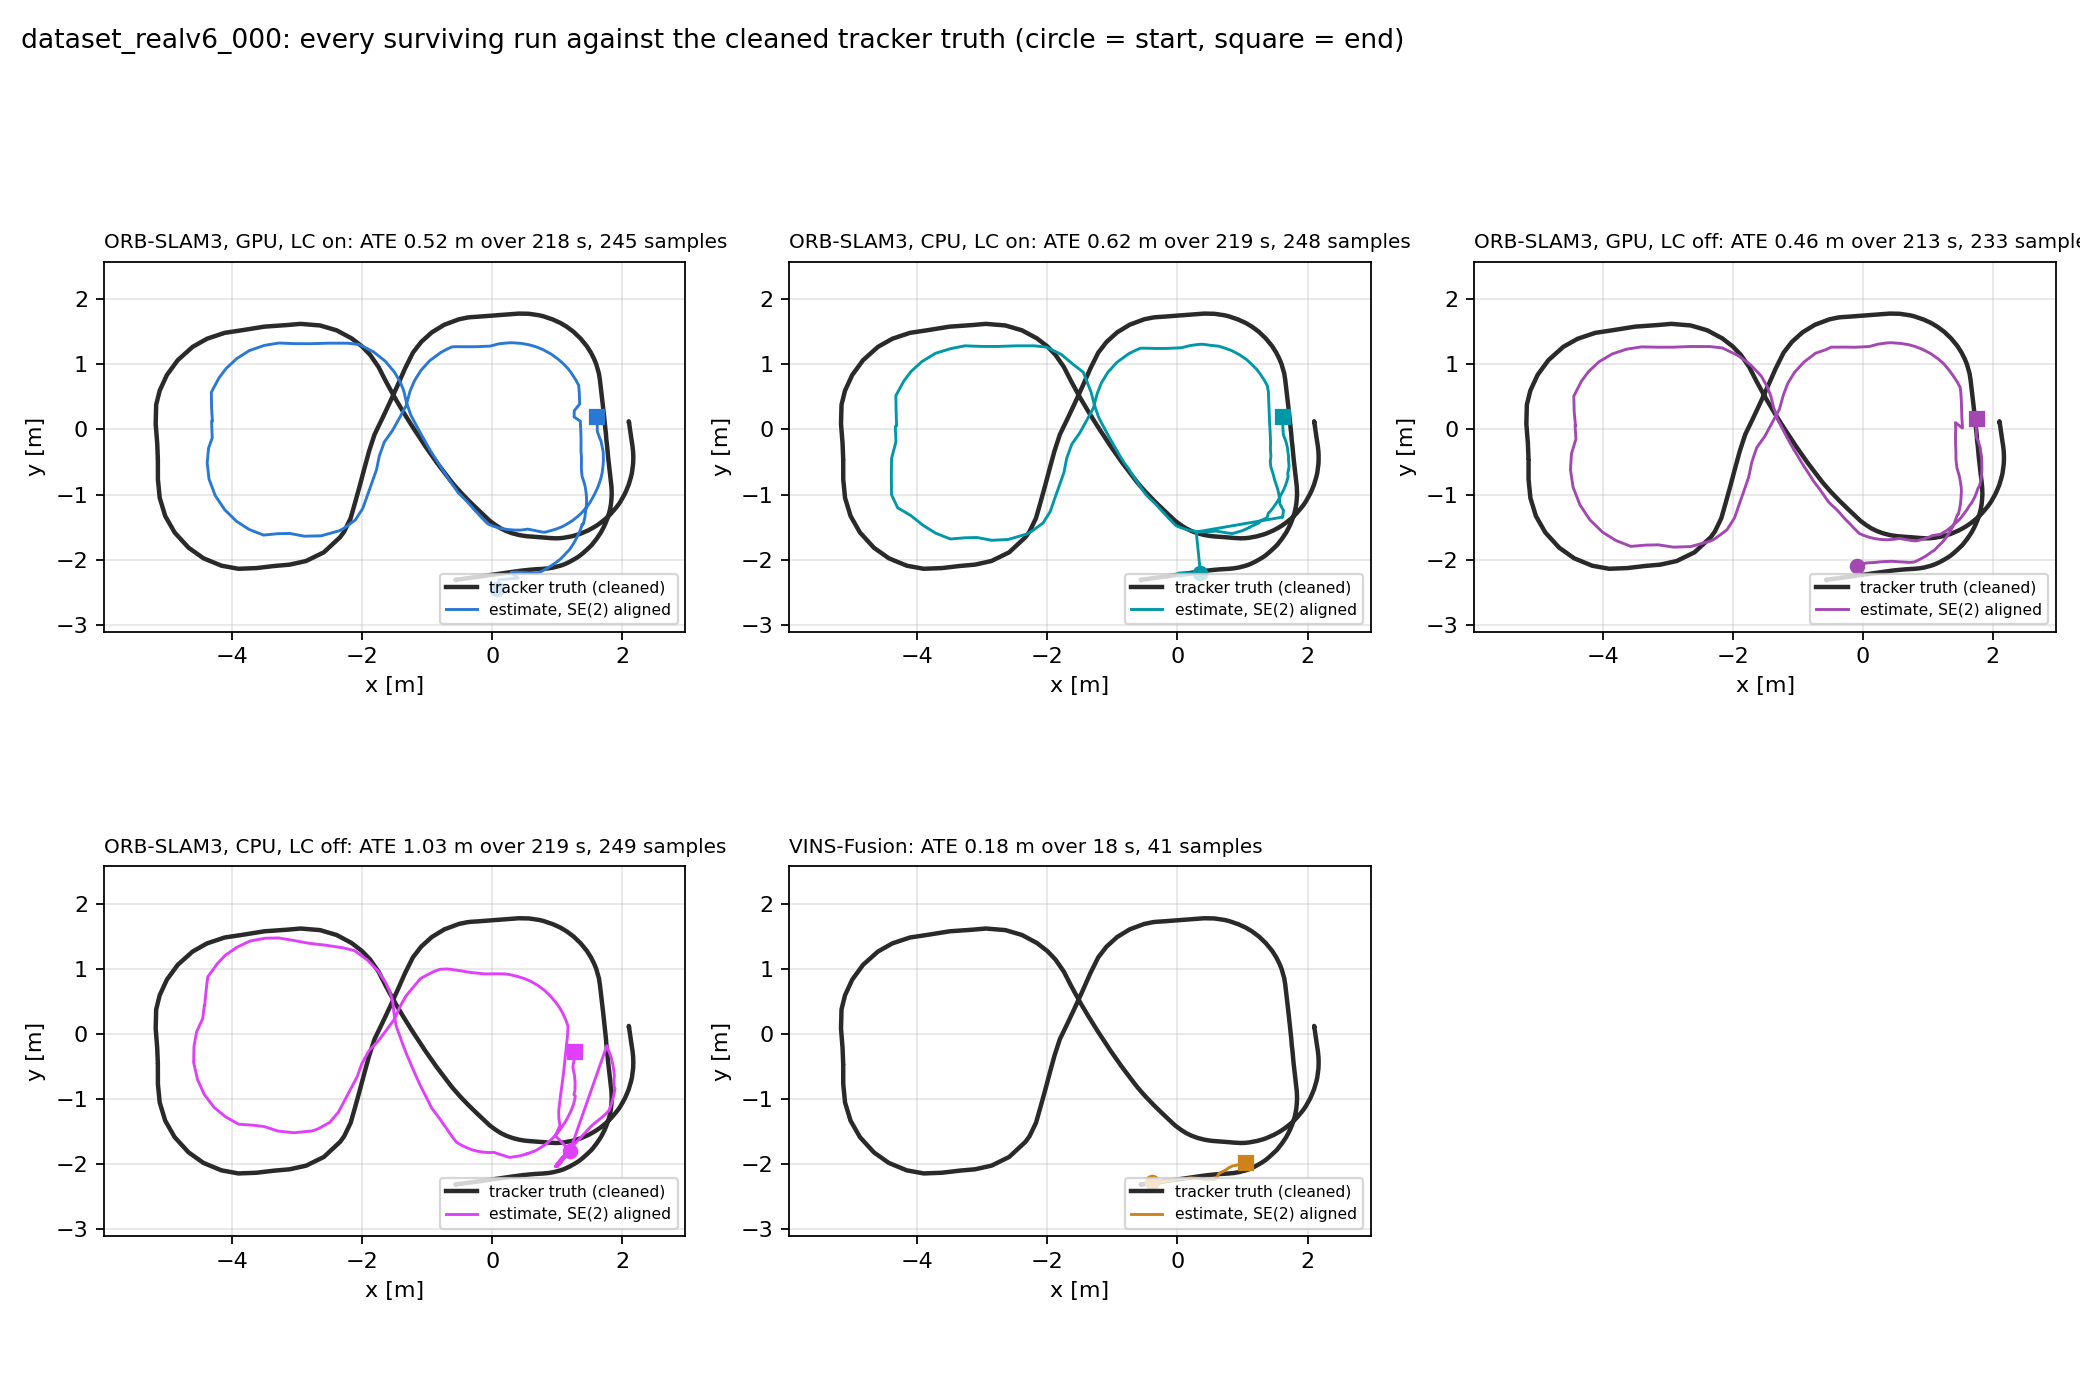
\includegraphics[width=\textwidth]{../../../output/compare/real/realv6-insights/fig_paths_light.png}
  \caption[Real runs against the cleaned tracker truth.]{Every run against the
  cleaned tracker truth after rigid SE(2)
  alignment, one panel per run: ORB-SLAM3 with GPU or CPU extractor and loop
  closing on or off, and VINS-Fusion's \SI{18}{\second}.}
  \label{fig:realv6-paths}
\end{figure}

\begin{table}[htbp]
\centering
\small
\caption[Realv6: raw versus cleaned tracker export.]{The same ORB-SLAM3 run (GPU, LC on) scored against the tracker export as delivered and with one sample removed (the \SI{5.2}{\metre} excursion at \SI{184.9}{\second}). The time offsets are the values the wheel-speed cross-correlation found on each export on 2 November (peak correlation 0.10 raw, 0.61 cleaned), applied here as pinned values. The cleaned truth still fails the gap rule (66 gaps above \SI{1}{\second}, tracker at \SI{1.7}{\hertz}).}
\label{tab:realv6-cleaning}
\begin{tabular}{lrrrrr}
\toprule
Truth & GT path [m] & offset [s] & ATE [m] & median [m] & path ratio \\
\midrule
as delivered & 36.8 & 4.38 & 1.174 & 0.851 & 0.65 \\
one sample removed & 27.1 & -4.14 & 0.519 & 0.437 & 0.85 \\
\bottomrule
\end{tabular}
\end{table}


\paragraph{Analysis.} The front end is what separates the runs. The GPU
extractor drops a third to a half of the frames and holds \SI{0.5}{\metre}; the
CPU extractor drops two thirds and loses a factor of two, one of its runs with a
\SI{2}{\metre} vertical excursion the tool flags as implausible and the other
with three resets and a half-second of lost tracking. Loop closing changes
nothing that the front end does not change more. The remaining resets are an
initialisation effect, two or three \repo{local_mapping_bad_imu} map resets
inside the first \SI{13}{\second} and none after (zero in the GPU run without
loop closing); after them the error is a slow wave between \SI{0.05}{} and
\SI{1}{\metre}, not an accumulating drift (\cref{fig:realv6-orb}), and it does
not rise while turning in any run (\cref{tab:realv6-turning}). The estimates are
a uniform \SIrange{12}{15}{\percent} smaller than the tracker's path, which the
unmeasured lever arm, a stereo-baseline error or a tracker scale error could
each explain. One tracker sample decides the headline: scored against the
export as delivered, the GPU run reads \SI{1.17}{\metre} with a path ratio of
0.65, because that sample adds \SI{10}{\metre} of false path and dominates the
time alignment (\cref{tab:realv6-cleaning}).

\begin{figure}[htbp]
  \centering
  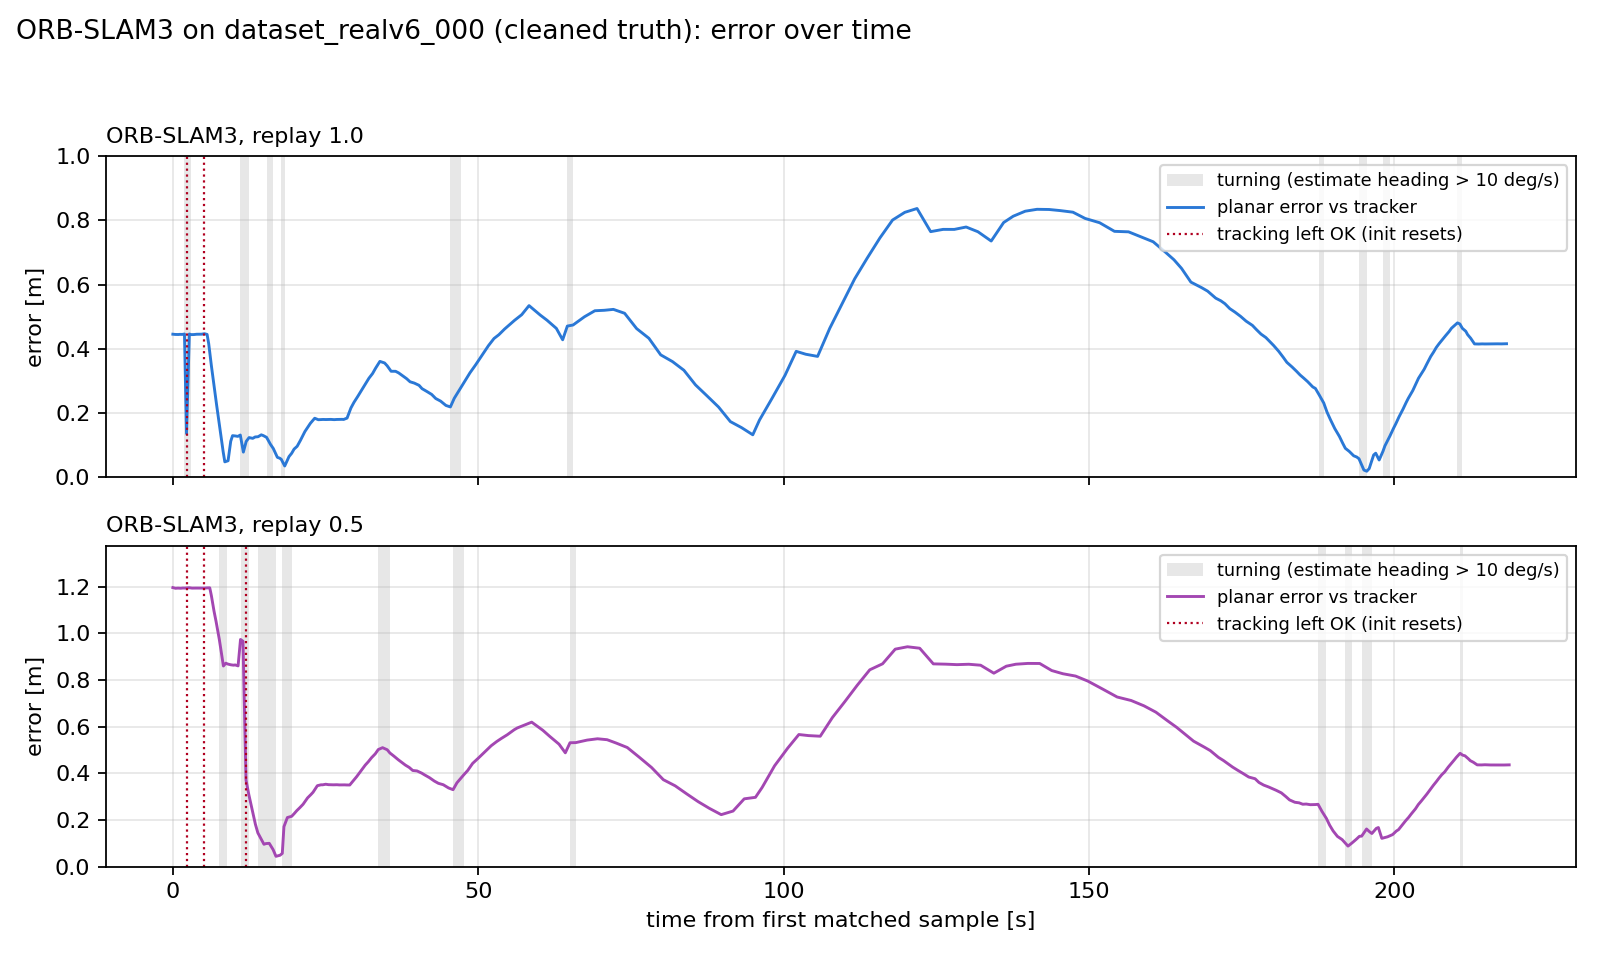
\includegraphics[width=\textwidth]{../../../output/compare/real/realv6-insights/fig_orb_timeline_light.png}
  \caption[ORB-SLAM3 planar error over the run.]{ORB-SLAM3 planar error over
  the run, one panel per configuration;
  grey bands are turns, dotted red the initialisation resets.}
  \label{fig:realv6-orb}
\end{figure}

\begin{table}[htbp]
\centering
\small
\caption[Realv6: ORB-SLAM3 drift while turning versus on straights.]{ORB-SLAM3 on \repo{dataset_realv6_000}, cleaned truth: growth rate of the planar error while the aligned estimate's heading changes faster than \SI{10}{\degree\per\second} and on straights, with the time in each state. Positive = error growing. One run per configuration, so no test is possible.}
\label{tab:realv6-turning}
\begin{tabular}{lrrrr}
\toprule
Run & turning [mm/s] & straight [mm/s] & time turning [s] & time straight [s] \\
\midrule
ORB-SLAM3, GPU, LC on & -11.2 & -0.3 & 23 & 171 \\
ORB-SLAM3, CPU, LC on & -29.8 & -1.4 & 23 & 162 \\
ORB-SLAM3, GPU, LC off & 4.9 & -2.1 & 11 & 185 \\
ORB-SLAM3, CPU, LC off & -49.9 & -0.9 & 20 & 182 \\
\bottomrule
\end{tabular}
\end{table}


The setting was reached by elimination. With the IMU noise densities copied
from the VINS file the estimator was unstable on this recording, running away
in its velocity state at a different place in each run; six out-of-bounds reads
in the library were fixed without removing it, every other candidate was varied
without removing it, and raising the IMU noise densities tenfold removed it in
every run since. Those earlier runs were overwritten and carry no number here;
the search is in the ORB-SLAM3 engineering record.

VINS-Fusion's failure is a delivery defect. The node received 3\,187 of 6\,601
frames but used 6\,498 of the 43\,494 IMU messages it received, reset 217 times
on \repo{imu_gap}, and stopped after \SI{19}{\second}; behind that defect the
configuration still fixes a gravity norm of \num{9.2642} against the
\SI{9.878}{\metre\per\second\squared} this IMU reads at rest.

\begin{table}[htbp]
\centering
\small
\caption[Realv6: the VINS-Fusion run.]{VINS-Fusion on \repo{dataset_realv6_000}, 3 November 2026 (\repo{config/wil/stereo_imu.yaml}, IMU noise $\times 10$, gravity norm still \num{9.2642} against the \SI{9.878}{\metre\per\second\squared} this IMU reads at rest). The scored span is the \SI{18}{\second} it tracked before its last reset and is not a result.}
\label{tab:realv6-vins}
\begin{tabular}{lr}
\toprule
Quantity & Value \\
\midrule
camera frames received (bag: 6\,601) & 3187 \\
IMU messages received / samples used & 43494 / 6498 \\
\repo{imu_gap} resets & 217 \\
poses written / span of poses & 286 / \SI{19}{\second} \\
tracker samples matched & 41 of 43 in span \\
ATE over the tracked span & \SI{0.18}{\metre} (not a result) \\
\bottomrule
\end{tabular}
\end{table}


\begin{figure}[htbp]
  \centering
  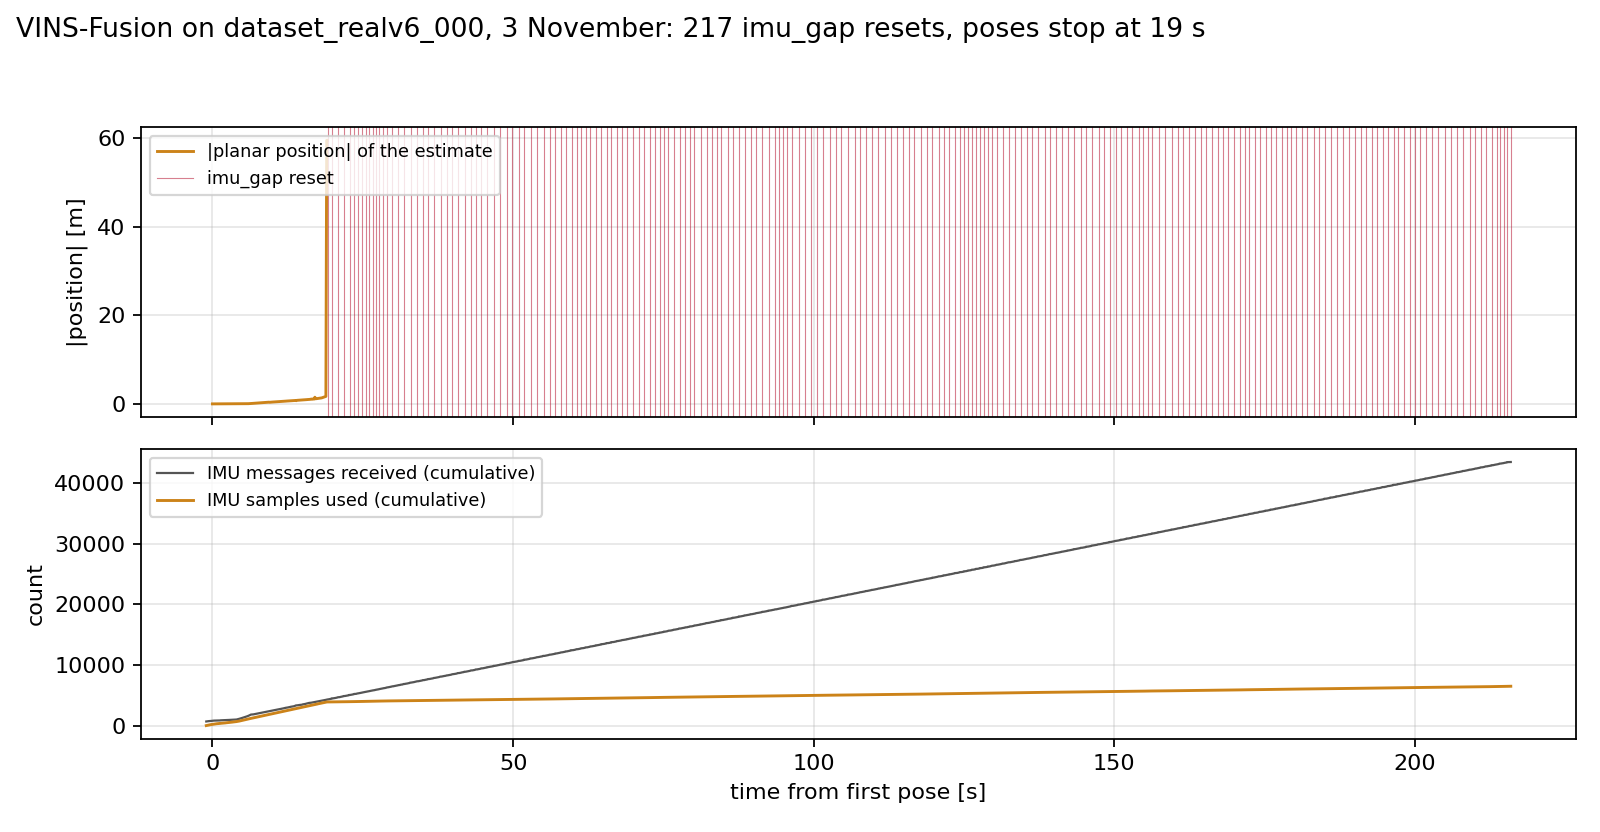
\includegraphics[width=\textwidth]{../../../output/compare/real/realv6-insights/fig_vins_light.png}
  \caption[VINS-Fusion resets and IMU sample use.]{VINS-Fusion: distance from
  origin with every \repo{imu_gap} reset
  marked, and IMU messages received against samples used.}
  \label{fig:realv6-vins}
\end{figure}

\paragraph{Second recording set, realv7.} Three further recordings of 3 November
2026 (\repo{dataset_realv7_000}, \repo{_001}, \repo{_002}: \SI{21.6}{},
\SI{31.7}{} and \SI{23.4}{\metre} over \SI{97}{}, \SI{134}{} and
\SI{104}{\second}) have tracker exports that pass every validity rule
(\SIrange{5}{6}{\hertz}, no gap, no step). Each carries the same four ORB-SLAM3
configurations and one VINS-Fusion run. As written in the live log
(\cref{tab:realv7-tilt}, \cref{fig:realv7-tilt}), a plane fitted to the
ORB-SLAM3 estimate lies within \SI{10}{\degree} of horizontal in three runs of
twelve and at \SIrange{88}{90}{\degree} in five, every \repo{000} run among
them, with the plane normal exactly a body axis in every run; scored as
written, those nine runs are not scorable.

The per-frame diagnostics give the mechanism. The IMU initialised
\SIrange{3}{4}{\second} after the first pose. The upstream rule that resets a
map with less than \SI{2}{\centi\metre} between consecutive keyframes in the
first ten seconds after the initialisation then discarded it, the robot being
still at rest. The new map starts in the camera frame of the reset instant, and
in it the re-initialisation was starved: upstream attempts it only with an
empty keyframe queue, which a keyframe every \SI{0.25}{\second} and
\SI{250}{\milli\second} of map-point creation per keyframe never allowed. The
IMU re-initialised after \SIrange{37}{92}{\second} in seven runs, never in two,
and early (\SI{6.7}{\second}) in the one run that was level. Until then the
estimate is stereo-only in a map whose vertical is the camera's $y$ axis, and
the late re-initialisation rotates the map under the already-written poses (the
\SIrange{1.9}{6.8}{\metre} steps).

A scorer-side repair was written while the cause was being found: it rotates
the pre-initialisation poses by the rotation measured at the initialisation
frame and levels each map's fitted plane, both without using the truth
(\cref{sec:method-realv7-repair}). It is kept for the record and is not used
for any result below, because the defect it worked around is now fixed in the
estimator; the one figure it produced that is still worth quoting is that on
\repo{000} it recovered \SIrange{0.252}{0.275}{\metre} from runs whose
estimates were lying on their side.

The fork's patch 15 adds two switches that attempt the initialisation with a
queued backlog and skip the low-motion reset for stereo. On 11 November 2026
all twelve runs were re-made with both active, and
\cref{tab:realv7-patch15} reports them scored \emph{raw}: neither of the two
repairs above was applied, which is the point of the table.

The upstream behaviour is gone from every run. The IMU initialised at
\SIrange{2.8}{4.7}{\second} and was retained; thirteen of the sixteen request
no map reset at all and the other three request one for a timestamp jump, not
for insufficient motion. The plane of the estimate now lies
\SIrange{0.2}{2.8}{\degree} from horizontal in every run against the
\SIrange{5}{90}{\degree} of \cref{tab:realv7-tilt}, and the vertical range
falls from as much as \SI{9.6}{} to at most \SI{1.00}{\metre}. Under the
scorer's own rules seven \repo{realv7} runs are now \status{completed} where
none was before and the other five are \status{partial}; the four
\repo{realv6} runs remain rejected, not for anything the estimator did but
because that recording's tracker export fails the validity rules.

The accuracy claim is narrower than the defect claim, and the three recordings
disagree. Set against the same configuration under upstream initialisation
\emph{after both repairs} --- each estimator at the best obtainable from it ---
patch 15 matches it on \repo{realv7_000} (\SIrange{0.251}{0.268}{} against
\SIrange{0.252}{0.275}{\metre}), is mixed on \repo{_001}, where two runs
improve and two worsen and one of those reaches \SI{1.278}{} against
\SI{0.817}{\metre}, and beats it on \repo{_002}
(\SIrange{0.172}{0.198}{} against \SIrange{0.472}{2.115}{\metre}, every one
of the four better than anything the repair obtained there) and on
\repo{realv6_000}, where all four improve
(\SIrange{0.404}{0.480}{} against \SIrange{0.457}{1.028}{\metre}) and the two
CPU runs improve most. The
defensible statement is therefore not that patch 15 is more accurate. It is
that patch 15 removes the need for the repair: it reaches on the raw estimate
what the stock estimator reaches only after its frame bookkeeping has been
corrected offline, and on the one recording the repair handled worst it
reaches considerably more. The
\SIrange{0.172}{0.198}{\metre} runs of \repo{_002} are the most accurate
real-robot ORB-SLAM3 figures in this report.

\begin{queried}[Open: what the improvement is owed to]
Two things differ between the two sets of runs, not one. Patch 15 is the
first; the second is that \repo{IMU.NoiseGyro} and \repo{IMU.NoiseAcc} were
inflated tenfold on 3 November, and no artefact records which values that
afternoon's runs used, because \repo{run_metadata.csv} stores the
configuration's path and not its contents. The loss of the tilt is
patch 15's: the upstream rule tests keyframe spacing below \SI{2}{\centi\metre}
within \SI{10}{\second} and cannot be influenced by an inertial noise density.
Any part of the accuracy difference is not separable on the present evidence.
One control run, the same bag at today's noise with both switches returned to
upstream, would separate them and has not been made.
\end{queried}

\begin{queried}[Provenance: the 3 November estimates are gone]
The re-runs overwrote \path{output/output_orb/real/dataset_realv7_00*/} in
place, so the pre-patch-15 estimates of all three recordings no longer exist
and neither \cref{tab:realv7-tilt} nor \cref{fig:realv7-tilt} can be
regenerated; the frozen copies beside the generator are the only record of the
behaviour this section reports as corrected. A run directory should be
written under a name that carries its configuration, so that a re-run cannot
overwrite the evidence for the behaviour it replaces.
\end{queried} VINS-Fusion
diverges on all three with the IMU stream intact (zero resets) and
\SIrange{40}{45}{\percent} of the frames received (\cref{tab:realv7-vins}); its
gravity norm has since been set to the measured \SI{9.886}{\metre\per\second\squared}.

% FROZEN 11 Nov 2026: the realv7_002 run directories this was computed from were
% overwritten by the patch-15 re-runs the same day, so realv7_002 CANNOT be
% regenerated. Do not replace this file from script/realv7_insights.py.
\begin{table}[htbp]
\centering
\scriptsize\setlength{\tabcolsep}{3pt}
\caption[Evidence of the initialisation defect: the plane of every estimate under stock ORB-SLAM3.]{ORB-SLAM3 on the three \repo{dataset_realv7} recordings, 3 November 2026 afternoon, same setting as the realv6 runs: the plane of each estimate as written in the live log, before any repair. ``Tilt'' is the angle between the plane fitted to the estimate's 3-D positions and the horizontal; ``off-plane'' the rms distance of the positions from that plane. A floor robot's estimate should be horizontal: a tilt near \SI{90}{\degree} means the poses were written while the map was not gravity-aligned (IMU not initialised; the vertical is then the camera's $y$ axis). The scores are in the patched runs of the real-robot results table.}
\label{tab:realv7-tilt}
\begin{tabular}{llrrrr}
\toprule
Recording & Run & tilt [\si{\degree}] & off-plane [m] & z range [m] & resets \\
\midrule
\repo{realv7_000} & GPU, LC on & \textcolor{flagred}{89.1} & 0.35 & 6.87 & 3 s \\
\repo{realv7_000} & GPU, LC off & \textcolor{flagred}{89.5} & 0.02 & 6.98 & 3 s \\
\repo{realv7_000} & CPU, LC on & \textcolor{flagred}{88.8} & 0.41 & 6.88 & 5 s \\
\repo{realv7_000} & CPU, LC off & \textcolor{flagred}{87.9} & 0.58 & 6.79 & 4 s \\
\addlinespace
\repo{realv7_001} & GPU, LC on & \textcolor{flagred}{88.8} & 0.05 & 9.64 & 4 s \\
\repo{realv7_001} & GPU, LC off & 6.1 & 1.12 & 5.77 & 3 s, 5 s \\
\repo{realv7_001} & CPU, LC on & 1.5 & 0.07 & 0.38 & 4 s \\
\repo{realv7_001} & CPU, LC off & \textcolor{flagred}{13.0} & 1.05 & 5.23 & 5 s \\
\addlinespace
\repo{realv7_002} & GPU, LC on & \textcolor{flagred}{37.7} & 0.87 & 4.08 & 3 s, 49 s, 59 s \\
\repo{realv7_002} & GPU, LC off & \textcolor{flagred}{59.7} & 0.83 & 4.80 & 49 s \\
\repo{realv7_002} & CPU, LC on & 5.2 & 0.73 & 2.94 & none \\
\repo{realv7_002} & CPU, LC off & \textcolor{flagred}{21.7} & 0.84 & 7.03 & none \\
\bottomrule
\end{tabular}
\end{table}


\begin{figure}[p]
  \centering
  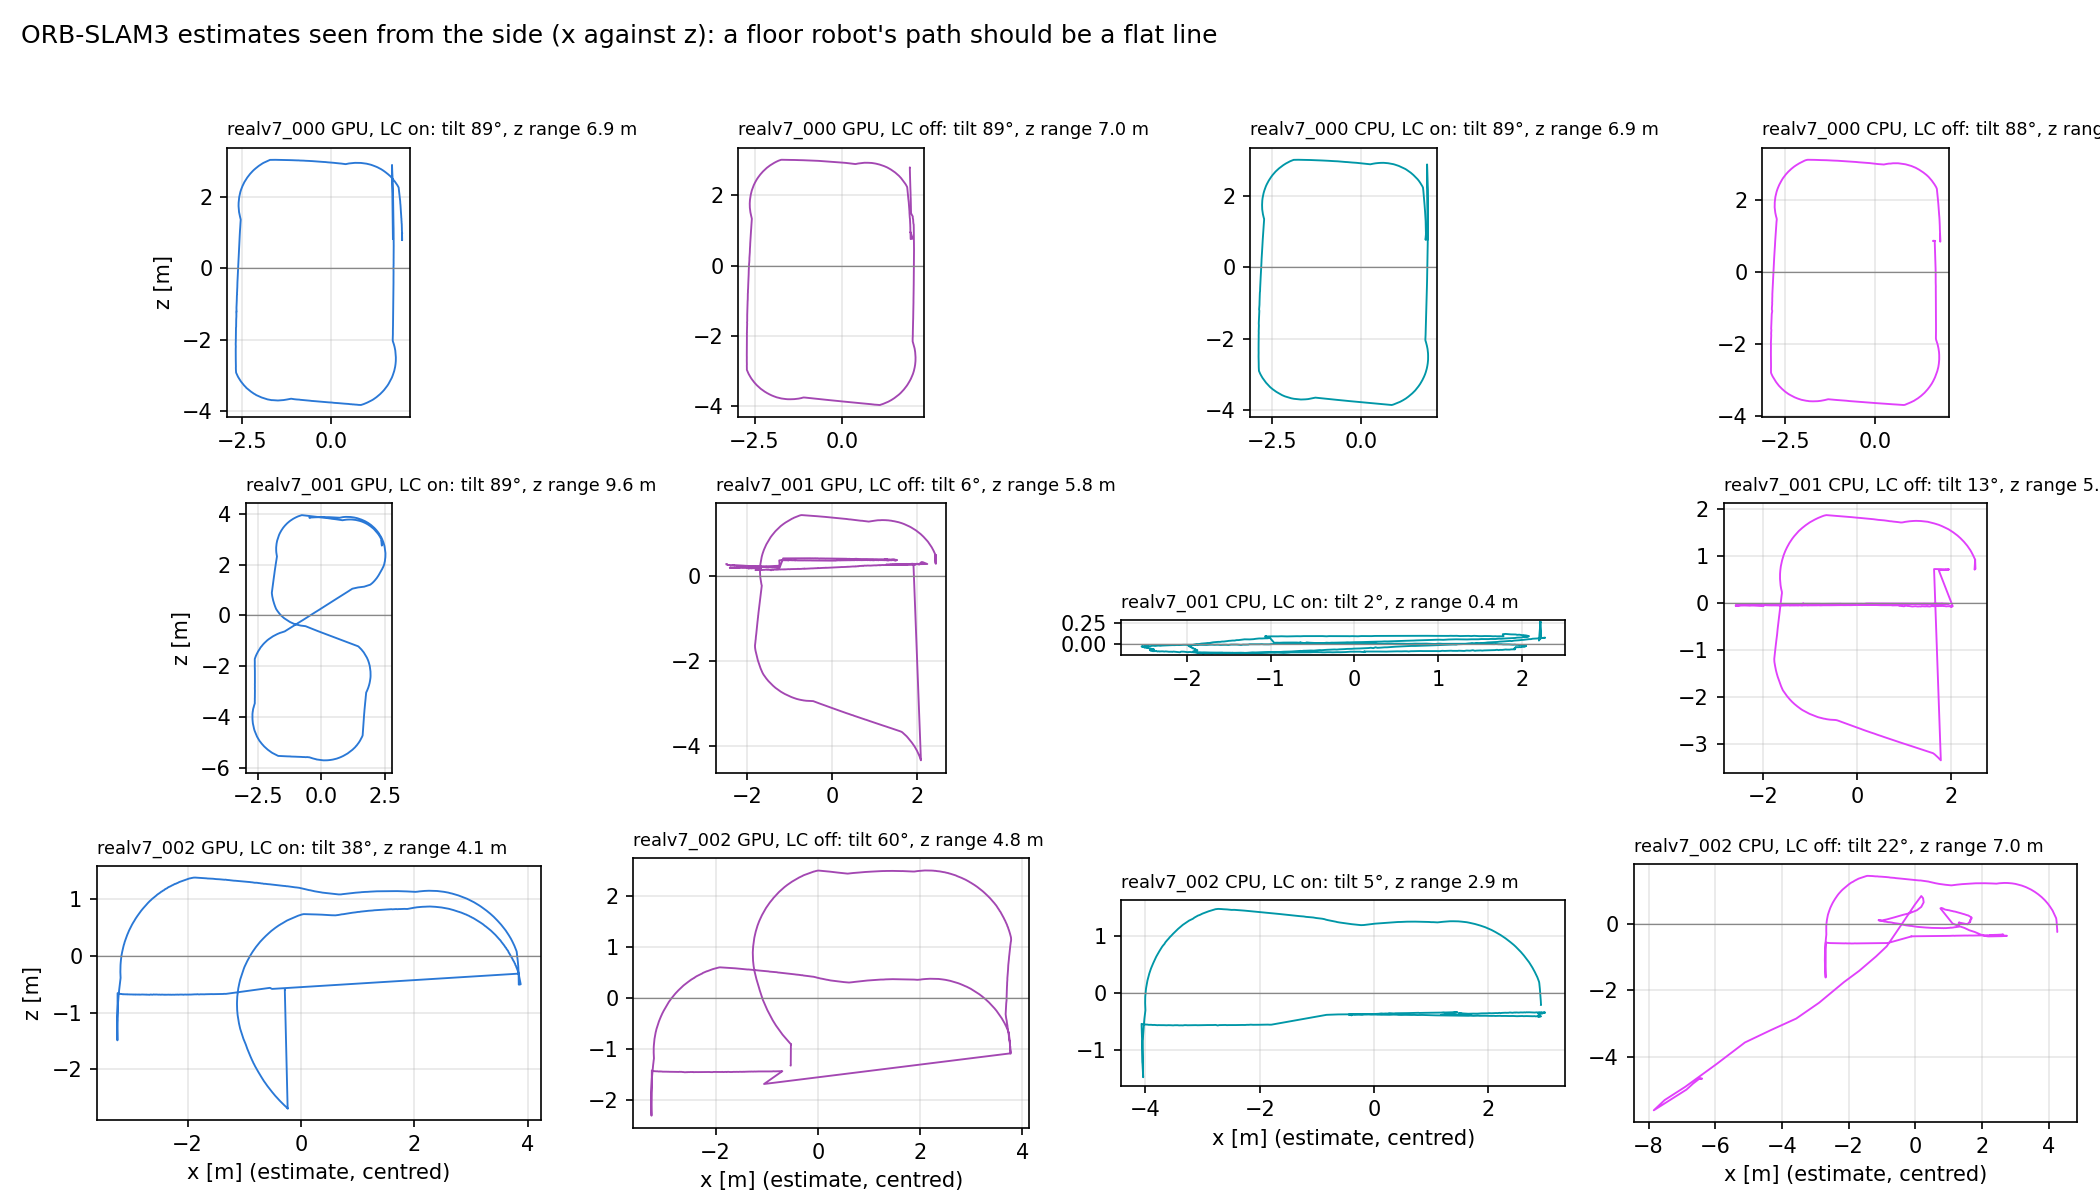
\includegraphics[width=\textwidth]{../../../output/compare/real/realv7-insights/fig_tilt_light_prepatch15.png}
  \caption[The twelve realv7 estimates as written in the live log.]{The twelve
  \repo{realv7} ORB-SLAM3 estimates as written in the live
  log, seen from the side ($x$ against $z$, centred); a floor robot's path should
  be a flat line. This is the defect that fork patch 15 removes; the estimates
  it produces instead are \cref{fig:realv7-paths-patch15}.}
  \label{fig:realv7-tilt}
\end{figure}

% Generated by script/realv7_patch15.py -- do not edit by hand.
\begin{table}[htbp]
\centering
\caption[Every real-robot run, with the upstream initialisation defect patched out.]{Every real-robot ORB-SLAM3 run on the four recordings that carry an independent planar reference, with fork patch 15 active (\repo{LocalMapping.resetOnLowMotion} 0, \repo{LocalMapping.initWithBacklog} 1) and scored \emph{raw}: neither \texttt{--join-imu-init} nor \texttt{--level-plane}, the repairs every other \repo{realv7} figure in this chapter depends on. ``Tilt'' and ``z range'' are measured the same way as in \cref{tab:realv7-tilt}, so the two are comparable. ``ATE before'' is the same configuration on the same recording on 3 November, scored raw. Front-end identity was confirmed from the median tracking latency (GPU \SIrange{41}{50}{\milli\second}, CPU \SIrange{104}{113}{\milli\second}), not from the run name. ``Stock + repair'' is the same configuration on the same recording on 3 November, under upstream initialisation and, for \repo{realv7}, only after the scorer-side frame repair that has since been retired: it is the fair comparison, each estimator at the best obtainable from it. For \repo{realv6_000}, which never showed the tilt and needed no repair, ``before'' is the same run scored against the same cleaned tracker export without the switches. Status is the scorer's: it rejects a run whose estimate spans more than \SI{1}{\metre} vertically, and it rejects every \repo{realv6} run because that recording's tracker export is \SI{1.7}{\hertz} and fails the validity rules written for the \SI{7}{\hertz} one, so its rows are diagnostics. Lever arm still unmeasured, so every value is provisional.}
\label{tab:realv7-patch15}
\small
\resizebox{\textwidth}{!}{%
\begin{tabular}{llrrr rr rrl}
\toprule
Recording & Run & IMU init [\si{\second}] & resets & tilt [\si{\degree}] & z range [\si{\metre}] & Kept & ATE [\si{\metre}] & Before [\si{\metre}] & status \\
\midrule
\repo{realv6_000} & GPU, LC on & 3.1 & 0 & 1.1 & 0.27 & 0.58 & 0.478 & 0.519 & failed \\
 & GPU, LC off & 4.5 & 1 & 1.2 & 0.33 & 0.51 & 0.404 & 0.457 & failed \\
 & CPU, LC on & 3.0 & 0 & 0.2 & 0.31 & 0.30 & 0.480 & 0.618 & failed \\
 & CPU, LC off & 2.8 & 0 & 1.8 & 0.36 & 0.28 & 0.456 & 1.028 & failed \\
\addlinespace
\repo{realv7_000} & GPU, LC on & 3.0 & 0 & 2.1 & 0.37 & 0.75 & 0.268 & 0.252 & partial \\
 & GPU, LC off & 3.0 & 0 & 2.0 & 0.36 & 0.69 & 0.251 & 0.259 & partial \\
 & CPU, LC on & 4.3 & 1 & 2.6 & 0.39 & 0.34 & 0.266 & 0.275 & partial \\
 & CPU, LC off & 4.3 & 1 & 1.6 & 0.34 & 0.32 & 0.259 & 0.261 & partial \\
\addlinespace
\repo{realv7_001} & GPU, LC on & 2.9 & 0 & 2.0 & 0.42 & 0.71 & 0.451 & 0.477 & completed \\
 & GPU, LC off & 4.7 & 0 & 1.7 & 0.45 & 0.67 & 1.278 & 0.817 & completed \\
 & CPU, LC on & 2.8 & 0 & 0.8 & 0.40 & 0.33 & 0.575 & 0.438 & completed \\
 & CPU, LC off & 2.9 & 0 & 2.0 & 0.42 & 0.32 & 0.442 & 0.558 & completed \\
\addlinespace
\repo{realv7_002} & GPU, LC on & 3.0 & 0 & 2.0 & 0.43 & 0.57 & 0.172 & 2.115 & completed \\
 & GPU, LC off & 3.1 & 0 & 2.5 & 0.45 & 0.63 & 0.198 & 2.079 & partial \\
 & CPU, LC on & 3.2 & 0 & 2.5 & 0.87 & 0.32 & 0.194 & 0.472 & completed \\
 & CPU, LC off & 3.2 & 0 & 2.8 & 1.00 & 0.31 & 0.198 & 1.675 & completed \\
\bottomrule
\end{tabular}}
\end{table}


\begin{figure}[p]
  \centering
  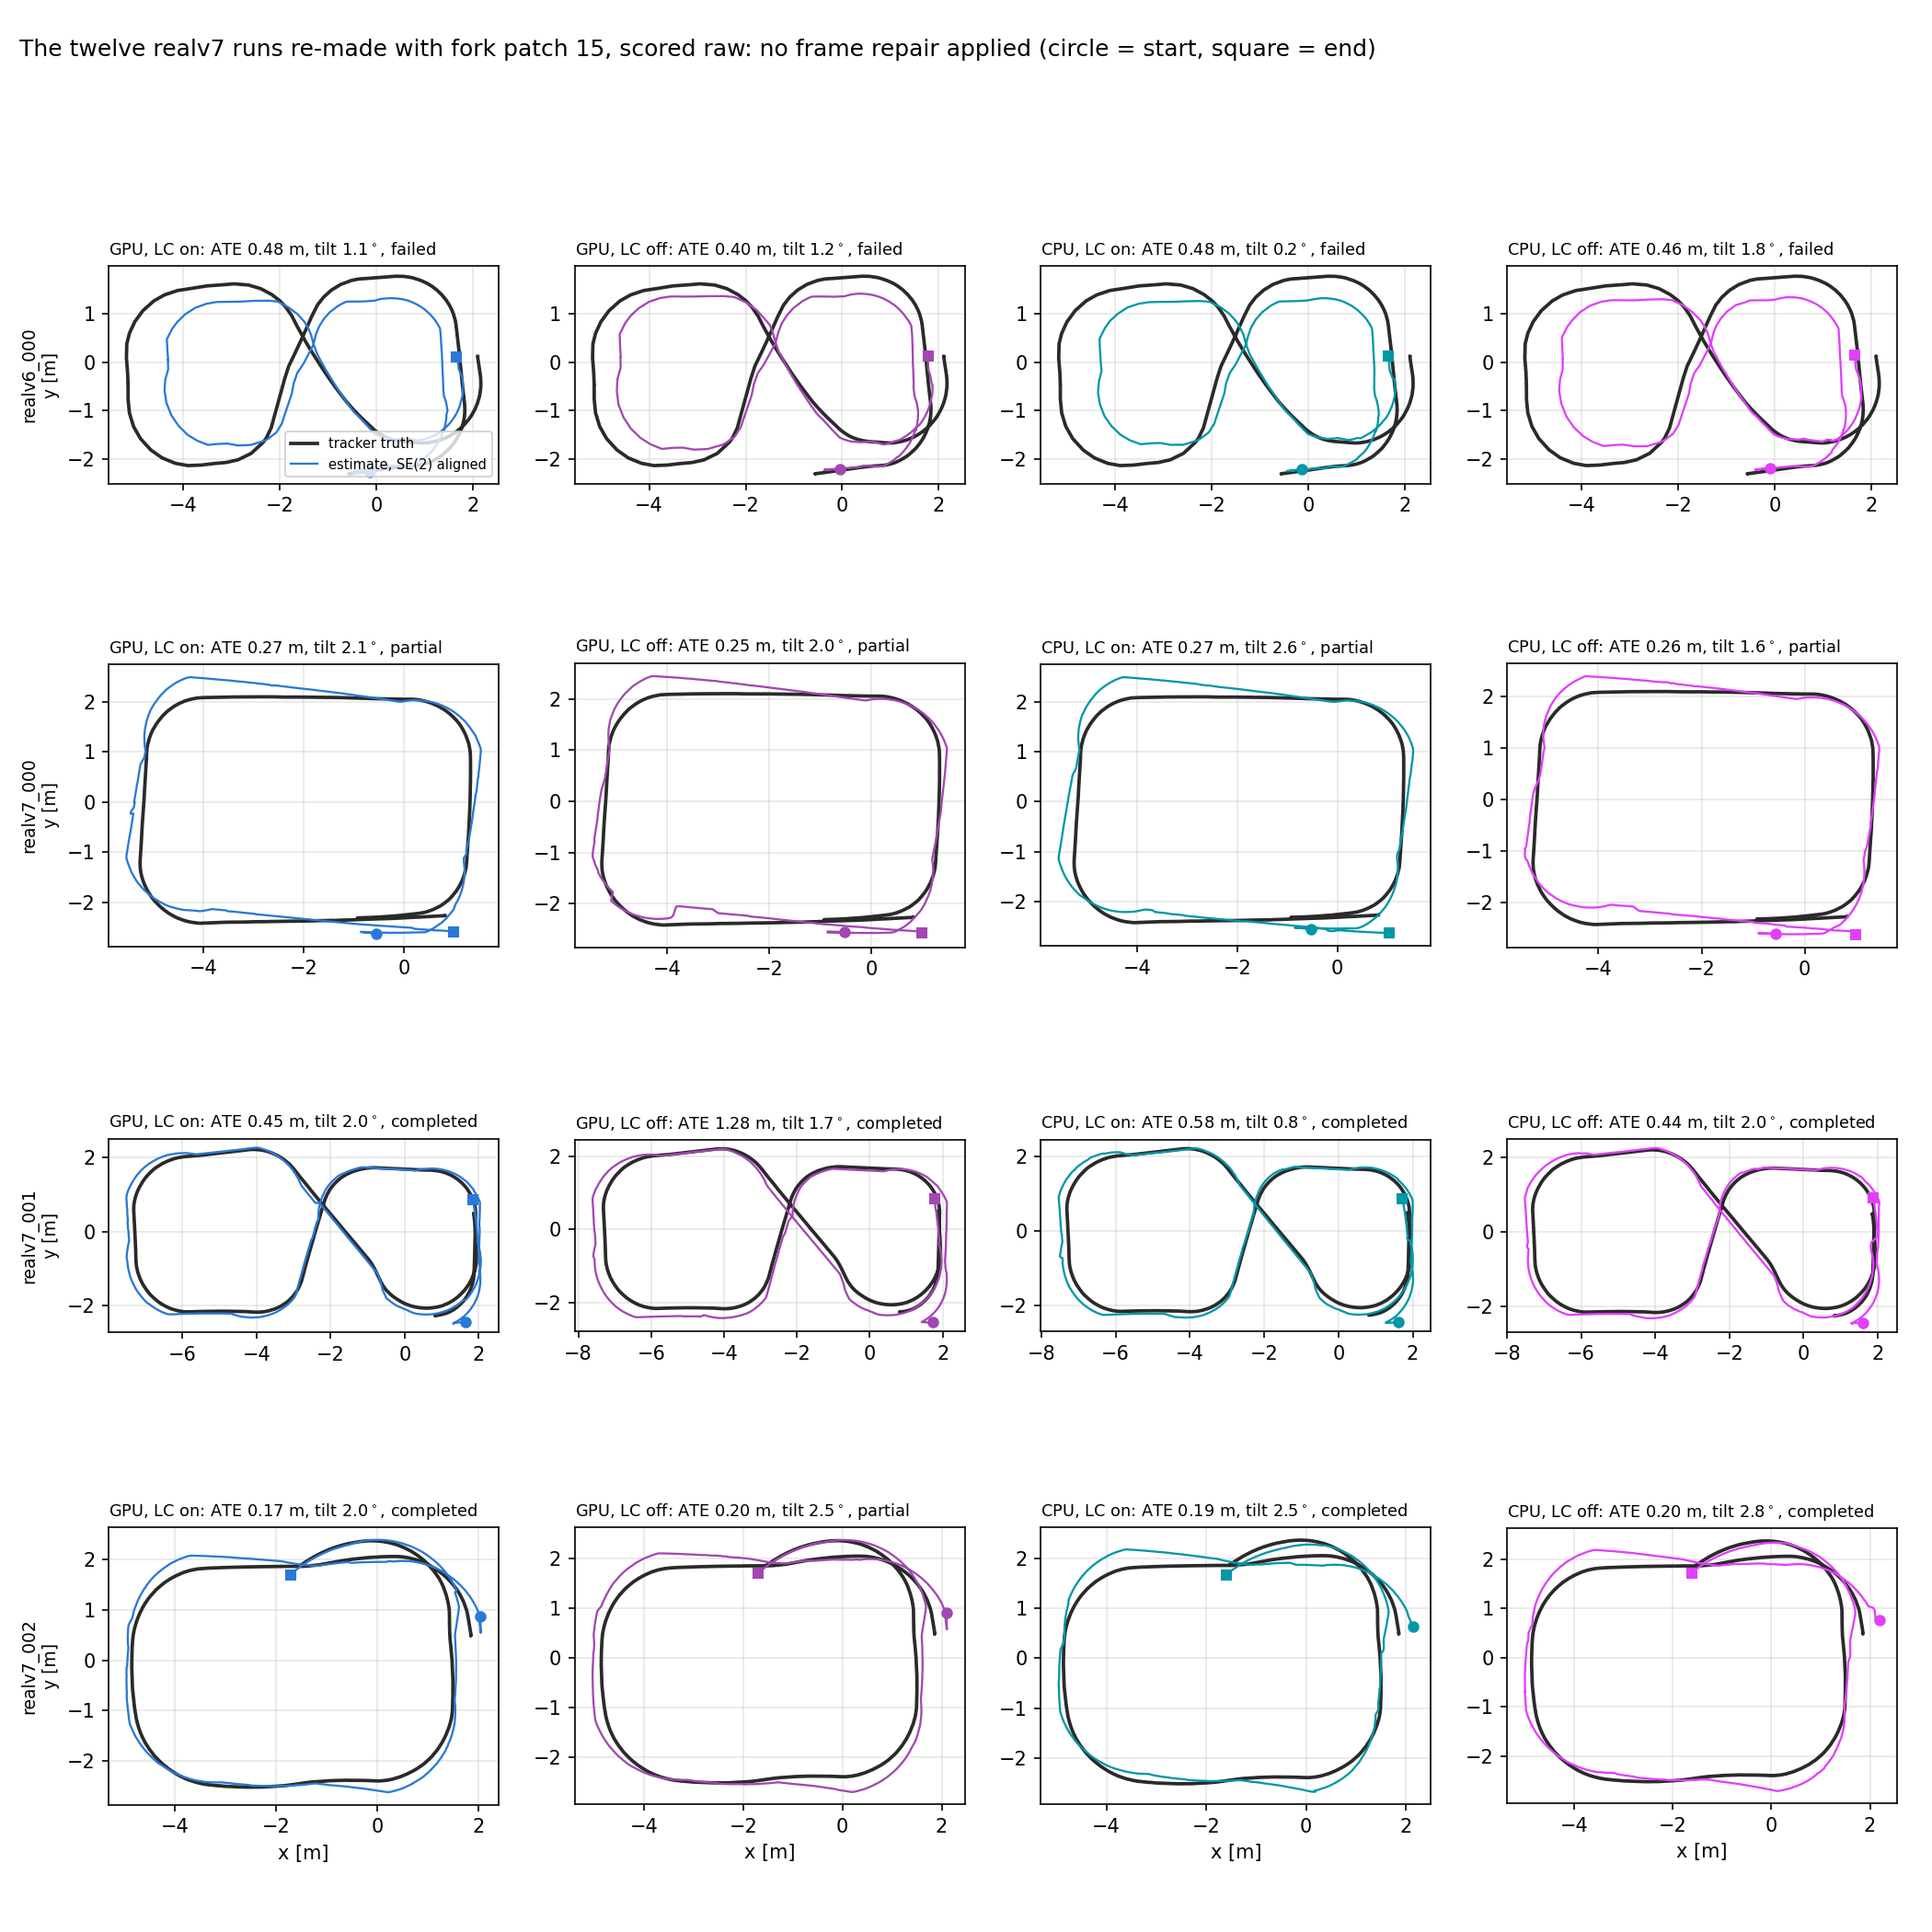
\includegraphics[width=\textwidth]{../../../output/compare/real/realv7-insights/fig_paths_patch15_light.png}
  \caption[Every real-robot run with patch 15, scored raw.]{Every real-robot
  ORB-SLAM3 run on the four recordings that carry an independent planar
  reference, with fork patch 15 active, against the tracker truth after rigid
  SE(2) alignment. No repair of
  any kind is applied: these are the estimates as the node wrote them, where
  those of \cref{fig:realv7-tilt} had to be levelled and rotated before they
  could be drawn at all. Each panel gives the planar ATE, the tilt of the
  fitted plane and the scorer's status.}
  \label{fig:realv7-paths-patch15}
\end{figure}

\begin{table}[htbp]
\centering
\small
\caption[Realv7: the VINS-Fusion runs.]{VINS-Fusion on the three \repo{dataset_realv7} recordings (\repo{config/wil/stereo_imu.yaml}, IMU noise $\times 10$, gravity norm \num{9.2642}). Frames received against the bag's count (\SI{30}{\hertz} over the recording), IMU use, resets, and where the estimate ended.}
\label{tab:realv7-vins}
\resizebox{\textwidth}{!}{%
\begin{tabular}{lrrrrr}
\toprule
Recording & frames received & IMU received / used & resets & z range [m] & $|p|$ at end [m] \\
\midrule
\repo{realv7_000} & 1155 of about 2663 & 17906 / 19053 & 0 & 12834403 & 37554 \\
\repo{realv7_001} & 1541 of about 3686 & 24809 / 26340 & 0 & 3701 & 15974 \\
\repo{realv7_002} & 1271 of about 2910 & 19368 / 20627 & 0 & 25937 & 5252 \\
\bottomrule
\end{tabular}}
\end{table}


\begin{queried}[Sparse reference]
The tracker ran at \SI{1.7}{\hertz} rather than its nominal \SI{7}{\hertz} on
\repo{realv6}, and
the validity rules were written for the faster export. Either the export has to
be re-captured at full rate or a rule for sparse references has to be written
before any value from this recording is quoted outside a diagnostic.
\end{queried}

\paragraph{Summary.} On the four real recordings the two families are in the
same accuracy class. Wheel+gyro dead reckoning, with one constant fitted on
\repo{realv7_000} and held, localises the robot to \SI{0.26}{} and
\SI{0.22}{\metre} on the other two \repo{realv7} recordings and
\SI{0.46}{\metre} on \repo{realv6}; ORB-SLAM3, with the upstream
initialisation defect patched out and scored raw, reads \SI{0.44}{},
\SI{0.17}{} and \SI{0.40}{\metre} on the same three. The baseline leads on
one, ties on one and is beaten on the third. The cause of the IMU staying
uninitialised for most of nine of the original twelve \repo{realv7} runs ---
an upstream map reset at the initialisation and a starved re-initialisation
--- is diagnosed, patched in the fork and now exercised on every run; what the
patch is shown to do is remove the need for the scorer's frame repair, not to
improve accuracy, which it matches on one recording, splits on a second and
improves on the other two. VINS-Fusion has no valid run on any recording,
through two delivery and configuration defects that are diagnosed and in part
corrected. The marker-to-IMU lever arm is unmeasured, so every figure here is
provisional, and \repo{realv6}'s tracker export fails the validity rules
written for the faster one, so its rows are diagnostics.

\textbf{Next action.} Run one \repo{realv7} recording with both initialisation
switches returned to upstream at the current inertial noise, which is the
control that separates patch 15 from the tenfold noise change made the same
week; re-run VINS-Fusion with the corrected gravity norm; measure the
marker-to-IMU lever arm, which every real figure in this chapter is
provisional on; and replace the fitted wheel-speed constant with a measured
one. Write each run under a directory name that carries its configuration, so
that no re-run overwrites the evidence it replaces.

\FloatBarrier

% =====================================================================
\FloatBarrier
\section{Experiment 2: Offline YOLO Detector Performance}
\label{sec:exp2}

\FloatBarrier
\subsection{Simulation}
\label{sec:yolo-performance}
\label{fig:yolo-ground-truth-overlay}
\label{sec:exp2-sim}

\slotstatus{completed}{Four realistic-warehouse recordings, 12\,698 left-camera
frames, scored on 7 November 2026 against projected simulator ground truth
with the four-class checkpoint
(\repo{weight/runs_1/detect/train/weights/best.pt}: bin, box, bucket,
forklift), whose fourth class fires on the pallet jacks that are the moving
objects of these recordings. Pooled precision 0.747; recall 0.502 over the
truth boxes the exemptions keep and 0.288 over every truth box;
moving-object recall 0.288. The walking people are simulator actors with no
pose and no class, so they are outside the score on both sides.}

\textbf{Objective.} Measure how well the project detector localises and
names warehouse objects, independently of either SLAM integration, so that
the dynamic filters of Experiment~3 have a known input quality; the
moving-object recall is the headline, because it is the ceiling of any
filtering benefit.

\textbf{Process.} \repo{script/yolo_eval.py} projected the collision mesh of
every model it has a class for into \repo{cam0} from the simulator's pose
stream to form truth boxes (the pallet jacks included, moving or parked), ran
the checkpoint at confidence 0.35 with NMS at IoU 0.5 on the GPU, matched
predictions greedily by class at IoU 0.5, and wrote per-frame and
per-detection records; twelve overlays per recording were inspected before
the aggregates were accepted. Truth boxes under 12 pixels or more than
\SI{70}{\percent} covered by nearer geometry are exempt (scored as neither hit
nor miss), and predictions on unlabelled box-like scenery (loaded shelves,
desks) are ignored. The three-class checkpoint of the retired evaluation is
not used: it has no class for the moving objects. The earlier evaluation on
the scripted worlds was retired on 6 November with its recordings and is not
cited.

\textbf{Datasets.} The four \repo{dataset_allsensor_realistic} recordings:
\repo{000} and \repo{001} static (U and I layout), \repo{002} and \repo{003}
with four pallet jacks on logistics jobs and four walking people. Ten pallet
jacks stand in each world, so the forklift class has truth in every recording
and \emph{moving} truth only in \repo{002} and \repo{003} (3\,333 and 4\,562
moving truth boxes). Sources: \path{output/yolo_eval/dataset_allsensor_realistic_*_4class/}
(\repo{yolo_eval.csv}, \repo{yolo_detections.csv}, \repo{yolo_confusion.csv},
\repo{overlay/}), \path{output/yolo_eval/summary_metrics.csv},
\path{output/compare/simulation/exp2-insights/}.

\textbf{Reporting rules.} Precision is over all retained predictions that
were not ignored; recall is quoted on two bases, over the truth boxes the
exemptions keep (the detector's task) and over every projected truth box
(what is physically in view); moving-object recall counts a truth box as
moving when its model moved more than \SI{0.05}{\metre} between frames.
Class metrics are conditional on a correct localisation.

\paragraph{Results.} \Cref{tab:exp2-summary}. The detector names what it
finds and finds about half of what the exemptions leave it: pooled
precision 0.747, recall 0.502 on the scored basis and 0.288 on the all-box
basis, class F1 0.994 conditional on a match. Moving pallet jacks are found
in 0.283 and 0.291 of their frames on \repo{002} and \repo{003}. The forklift
class is the weakest on the all-box basis (recall 0.12 to 0.18 against 0.18
to 0.45 for the others, \cref{tab:e2i-class}), and the box class carries
\SIrange{34}{70}{\percent} of the false positives.

\begin{table}[htbp]
\centering
\caption[Detector scores per recording and pooled.]{Detector scores per
recording and pooled, four-class checkpoint,
confidence 0.35, matching IoU 0.5. ``Truth'' counts every projected box and
``exempt'' those under 12 pixels or more than \SI{70}{\percent} covered;
$R_{\mathrm{scored}}$ is recall over the rest, $R_{\mathrm{all}}$ over every
box, $R_{\mathrm{mov}}$ over the moving truth boxes.}
\label{tab:exp2-summary}
\small
\resizebox{\textwidth}{!}{%
\begin{tabular}{lrrrrrrrrr}
\toprule
Recording & Frames & Truth & Exempt & Pred. & TP & FP & $P$ & $R_{\mathrm{scored}}$ & $R_{\mathrm{all}}$ / $R_{\mathrm{mov}}$ \\
\midrule
\repo{realistic_000} & 3\,805 & 38\,401 & 16\,157 & 16\,673 & 10\,940 & 2\,693 & 0.802 & 0.492 & 0.285 / --- \\
\repo{realistic_001} & 2\,937 & 33\,260 & 14\,286 & 14\,359 & 8\,834 & 3\,907 & 0.693 & 0.466 & 0.266 / --- \\
\repo{realistic_002} & 2\,409 & 28\,049 & 10\,907 & 13\,002 & 8\,821 & 2\,332 & 0.791 & 0.515 & 0.314 / 0.283 \\
\repo{realistic_003} & 3\,547 & 40\,498 & 18\,235 & 19\,148 & 11\,852 & 4\,757 & 0.714 & 0.532 & 0.293 / 0.291 \\
\midrule
Pooled & 12\,698 & 140\,208 & 59\,585 & 63\,182 & 40\,447 & 13\,689 & 0.747 & 0.502 & 0.288 / 0.288 \\
\bottomrule
\end{tabular}}
\end{table}

\paragraph{Analysis.} The misses are a size effect and the false positives
are near misses. Frame-level recall rises monotonically with the truth-box
side, from 0.02 at 24--32 pixels to 0.64 above 192 pixels
(\cref{tab:e2i-size}, \cref{fig:exp2-size}); at object level every object is
found in most of the frames where its box is large, and the moving pallet
jacks follow the same curve as the parked ones, so the moving-object recall
of 0.29 is what the pallet jacks' typical distance from the camera gives,
not a motion effect. Of the unmatched predictions, \SIrange{74}{79}{\percent}
overlap the right object below the IoU threshold and only
\SIrange{8}{9}{\percent} land on nothing (\cref{tab:e2i-fp},
\cref{fig:exp2-fp}): a looser matching threshold would move most false
positives into the hits, and a filter that masks by box does not care which.
The misses come as flicker rather than blindness: \SIrange{39}{47}{\percent}
of the gaps between consecutive detections of one object are a single frame,
and gaps longer than \SI{2}{\second} hold \SIrange{20}{32}{\percent} of the
misses (\cref{tab:e2i-miss}). Raising the confidence threshold buys
precision at a steep price in recall: at 0.75 precision is 0.84 to 0.91 and
moving-object recall 0.16 to 0.20 (\cref{tab:e2i-threshold}).

\begin{table}[htbp]
\centering
\scriptsize
\setlength{\tabcolsep}{3pt}
\caption[Recall against truth-box size.]{Recall against truth-box size, pooled over the four recordings. Frame level: the frame's truth boxes are binned by the frame's mean truth-box side (square root of the mean truth area; the per-box truth is not logged), recall is TP/(TP+FN) of those frames. Object level: each object's median matched-box side; a miss is a frame inside a gap shorter than \SI{2}{\second} between two matches of that object, so objects that leave the view are not charged. Moving: object moving in at least half of its matched frames. Source: \path{recall_by_size.csv}.}
\label{tab:e2i-size}
\resizebox{\textwidth}{!}{%
\begin{tabular}{lrrrrrrr}
\toprule
Side [px] & \multicolumn{3}{c}{frame level} & \multicolumn{4}{c}{object level} \\
 & boxes & recall & R$_{\mathrm{mov}}$ / R$_{\mathrm{stat}}$ & objects mov/stat & frames & R$_{\mathrm{mov}}$ & R$_{\mathrm{stat}}$ \\
\midrule
0--24 & 0 & --- & --- / --- & 0/1 & 21 & --- & 0.24 \\
24--32 & 745 & 0.02 & --- / 0.02 & 1/1 & 932 & 0.96 & 0.93 \\
32--48 & 30027 & 0.10 & 0.16 / 0.10 & 0/18 & 7120 & --- & 0.79 \\
48--64 & 29454 & 0.18 & 0.11 / 0.18 & 3/17 & 7453 & 0.89 & 0.72 \\
64--96 & 37685 & 0.30 & 0.35 / 0.30 & 0/42 & 14312 & --- & 0.80 \\
96--128 & 21342 & 0.43 & 0.56 / 0.42 & 2/39 & 9856 & 0.53 & 0.85 \\
128--192 & 17840 & 0.54 & 0.70 / 0.53 & 3/45 & 9524 & 0.87 & 0.85 \\
192--$\infty$ & 3115 & 0.64 & 0.60 / 0.64 & 0/14 & 2794 & --- & 0.83 \\
\bottomrule
\end{tabular}}
\end{table}

\begin{table}[htbp]
\centering
\scriptsize
\setlength{\tabcolsep}{3pt}
\caption[What the unmatched predictions are.]{What the unmatched predictions are, per recording. An unmatched prediction is a \emph{duplicate} when it overlaps a matched prediction of the same class by IoU $\ge 0.5$; a \emph{near miss} when its best IoU with an unmatched truth box of its class is in $[0.2, 0.5)$; \emph{slight overlap} when that IoU is in $(0, 0.2)$; \emph{no overlap} when it touches no truth box. The scorer excludes the predictions that land on unlabelled scenery (\emph{ignored}); they are counted here from the per-frame totals because the per-box file does not flag them, so the four categories sum to unmatched, not to scored false positives. ``At border'': the box touches an image edge. Source: \path{output/compare/simulation/exp2-insights/fp_anatomy.csv}.}
\label{tab:e2i-fp}
\resizebox{\textwidth}{!}{%
\begin{tabular}{lrrrrrrrr}
\toprule
Recording & unmatched & scored FP & ignored & duplicate & near miss & slight & none & at border \\
 & & & (scenery) & & [0.2,0.5) & (0,0.2) & 0 & \\
\midrule
\repo{dataset_allsensor_realistic_000_4class} & 5210 & 2693 & 3040 & 2 (0\,\%) & 3994 (77\,\%) & 745 (14\,\%) & 469 (9\,\%) & 12\,\% \\
\repo{dataset_allsensor_realistic_001_4class} & 5229 & 3907 & 1618 & 0 (0\,\%) & 4330 (83\,\%) & 626 (12\,\%) & 273 (5\,\%) & 13\,\% \\
\repo{dataset_allsensor_realistic_002_4class} & 3860 & 2332 & 1849 & 1 (0\,\%) & 2860 (74\,\%) & 684 (18\,\%) & 315 (8\,\%) & 13\,\% \\
\repo{dataset_allsensor_realistic_003_4class} & 6849 & 4757 & 2539 & 2 (0\,\%) & 5101 (74\,\%) & 1213 (18\,\%) & 533 (8\,\%) & 12\,\% \\
\bottomrule
\end{tabular}}
\end{table}

\begin{table}[htbp]
\centering
\small
\caption[Structure of the misses.]{Structure of the misses, per recording, from the gaps between consecutive matches of the same object (gaps under \SI{2}{\second} only). ``Single-frame'' is the share of gaps one frame long; ``in long gaps'' the share of the gap frames that lie in gaps of \SI{1}{\second} or more. ``Short-gap misses / FN'' compares the misses this reading finds with the scorer's total false negatives: the remainder are misses at the ends of tracks or in gaps longer than \SI{2}{\second}, which this reading cannot separate from objects leaving the view. ``Objects under 0.5'': objects with at least 30 frames whose in-track recall is below one half. Source: \path{miss_structure.csv}.}
\label{tab:e2i-miss}
\resizebox{\textwidth}{!}{%
\begin{tabular}{lrrrrrrr}
\toprule
Recording & objects & gaps & median & p90 & single-frame & in long gaps & short-gap misses / FN \\
 & & & [frames] & [frames] & & & \\
\midrule
\repo{dataset_allsensor_realistic_000_4class} & 45 (4 under 0.5) & 513 & 2 & 9 & 47\,\% & 20\,\% & 2038 / 27461 (7\,\%) \\
\repo{dataset_allsensor_realistic_001_4class} & 51 (12 under 0.5) & 513 & 2 & 17 & 40\,\% & 24\,\% & 2952 / 24426 (12\,\%) \\
\repo{dataset_allsensor_realistic_002_4class} & 45 (7 under 0.5) & 288 & 2 & 8 & 44\,\% & 30\,\% & 1330 / 19228 (7\,\%) \\
\repo{dataset_allsensor_realistic_003_4class} & 45 (4 under 0.5) & 646 & 2 & 15 & 39\,\% & 32\,\% & 3658 / 28646 (13\,\%) \\
\bottomrule
\end{tabular}}
\end{table}

\begin{table}[htbp]
\centering
\scriptsize
\setlength{\tabcolsep}{3pt}
\caption[Score-threshold sweep.]{Score-threshold sweep over the retained predictions. Precision, recall and moving-object recall if every prediction below the threshold were discarded; the logged operating point is \num{0.35}, and nothing below it was retained, so the sweep can only go up. Matching is not re-run, so a discarded higher-scored box cannot free its truth for a lower-scored one; the values are therefore lower bounds on recall by a small margin. Source: \path{threshold_sweep.csv}.}
\label{tab:e2i-threshold}
\resizebox{\textwidth}{!}{%
\begin{tabular}{lrrrrrrrrrrrr}
\toprule
Threshold & \multicolumn{3}{c}{\repo{realistic_000}} & \multicolumn{3}{c}{\repo{realistic_001}} & \multicolumn{3}{c}{\repo{realistic_002}} & \multicolumn{3}{c}{\repo{realistic_003}} \\
 & P & R & R$_{\mathrm{mov}}$ & P & R & R$_{\mathrm{mov}}$ & P & R & R$_{\mathrm{mov}}$ & P & R & R$_{\mathrm{mov}}$ \\
\midrule
0.35 & 0.80 & 0.28 & 0.00 & 0.69 & 0.27 & 0.00 & 0.79 & 0.31 & 0.28 & 0.71 & 0.29 & 0.29 \\
0.45 & 0.82 & 0.28 & 0.00 & 0.72 & 0.26 & 0.00 & 0.82 & 0.31 & 0.27 & 0.74 & 0.28 & 0.28 \\
0.55 & 0.85 & 0.27 & 0.00 & 0.74 & 0.25 & 0.00 & 0.85 & 0.30 & 0.26 & 0.76 & 0.27 & 0.26 \\
0.65 & 0.87 & 0.25 & 0.00 & 0.77 & 0.23 & 0.00 & 0.88 & 0.28 & 0.23 & 0.79 & 0.24 & 0.23 \\
0.75 & 0.89 & 0.21 & 0.00 & 0.81 & 0.19 & 0.00 & 0.91 & 0.23 & 0.20 & 0.84 & 0.20 & 0.16 \\
0.85 & 0.94 & 0.12 & 0.00 & 0.86 & 0.08 & 0.00 & 0.94 & 0.11 & 0.09 & 0.93 & 0.09 & 0.06 \\
\bottomrule
\end{tabular}}
\end{table}

\begin{table}[htbp]
\centering
\scriptsize
\setlength{\tabcolsep}{3pt}
\caption[Misses and false positives by class.]{Misses and false positives by class, per recording, from the scorer's class-agnostic confusion counts. Recall is the share of truth boxes of the class associated with any prediction; FP share is the class's share of the recording's background-row predictions. The pallet jack is not a class of the loaded 3-class weights and is an ignore region, so it does not appear. Source: \path{output/yolo_eval/dataset_allsensor_realistic_*_4class/yolo_confusion.csv}.}
\label{tab:e2i-class}
\resizebox{\textwidth}{!}{%
\begin{tabular}{llrrrrrrrrrrrr}
\toprule
 & & \multicolumn{3}{c}{\repo{realistic_000}} & \multicolumn{3}{c}{\repo{realistic_001}} & \multicolumn{3}{c}{\repo{realistic_002}} & \multicolumn{3}{c}{\repo{realistic_003}} \\
Class & & truth & recall & FP share & truth & recall & FP share & truth & recall & FP share & truth & recall & FP share \\
\midrule
bin & & 4219 & 0.30 & 0.09 & 1072 & 0.18 & 0.00 & 3038 & 0.40 & 0.05 & 1624 & 0.00 & 0.04 \\
box & & 15541 & 0.22 & 0.34 & 19658 & 0.32 & 0.70 & 11161 & 0.45 & 0.46 & 20068 & 0.35 & 0.51 \\
bucket & & 11428 & 0.44 & 0.29 & 6529 & 0.21 & 0.07 & 6515 & 0.26 & 0.19 & 10816 & 0.35 & 0.16 \\
forklift & & 7213 & 0.18 & 0.27 & 6001 & 0.17 & 0.22 & 7335 & 0.12 & 0.30 & 7990 & 0.15 & 0.29 \\
\bottomrule
\end{tabular}}
\end{table}


\begin{figure}[htbp]
  \centering
  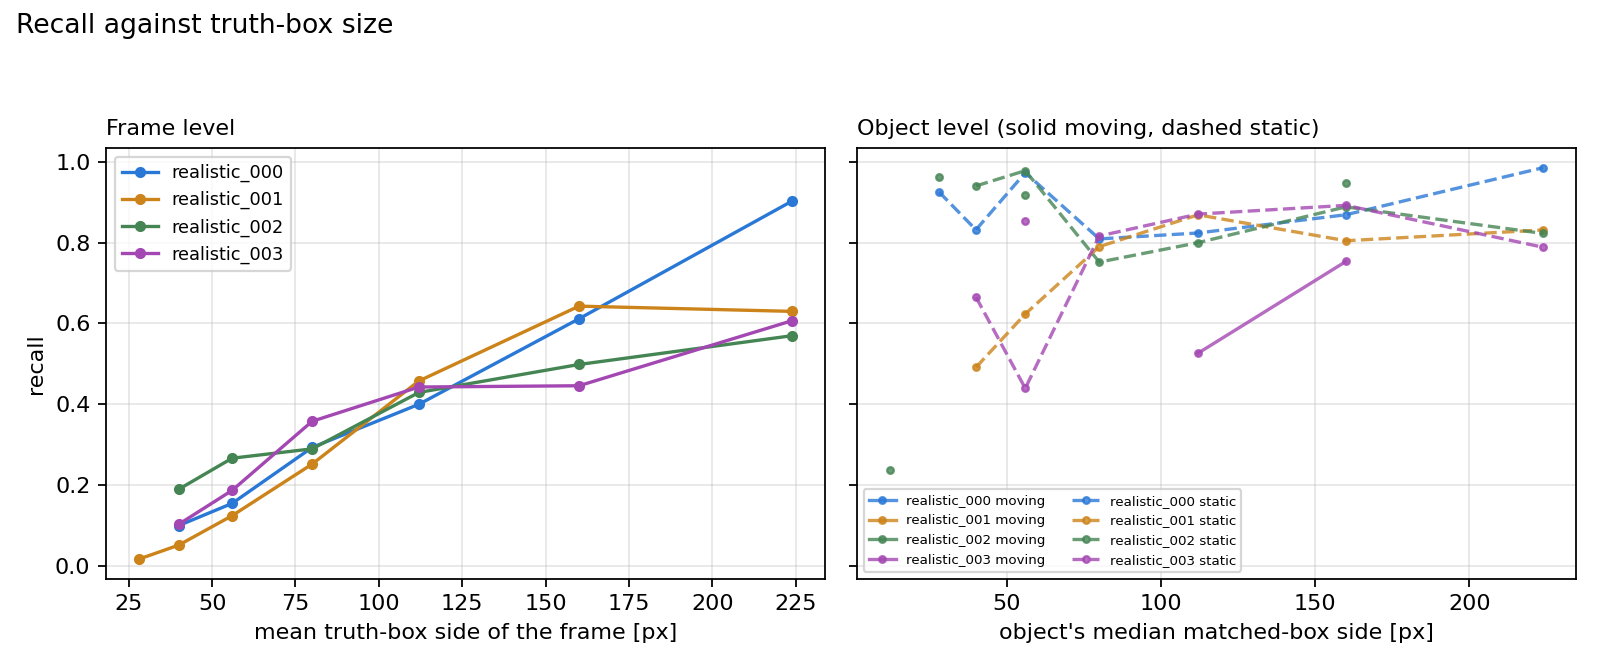
\includegraphics[width=\textwidth]{figures/yolo_fig_size.png}
  \caption[Recall against truth-box size.]{Recall against truth-box size: per
  frame (left, the frame's mean
  truth-box side) and per object (right, the object's median matched-box
  side; solid moving, dashed parked). The curves of the four recordings
  coincide, and the moving pallet jacks lie on the parked objects' curve.}
  \label{fig:exp2-size}
\end{figure}
\begin{figure}[htbp]
  \centering
  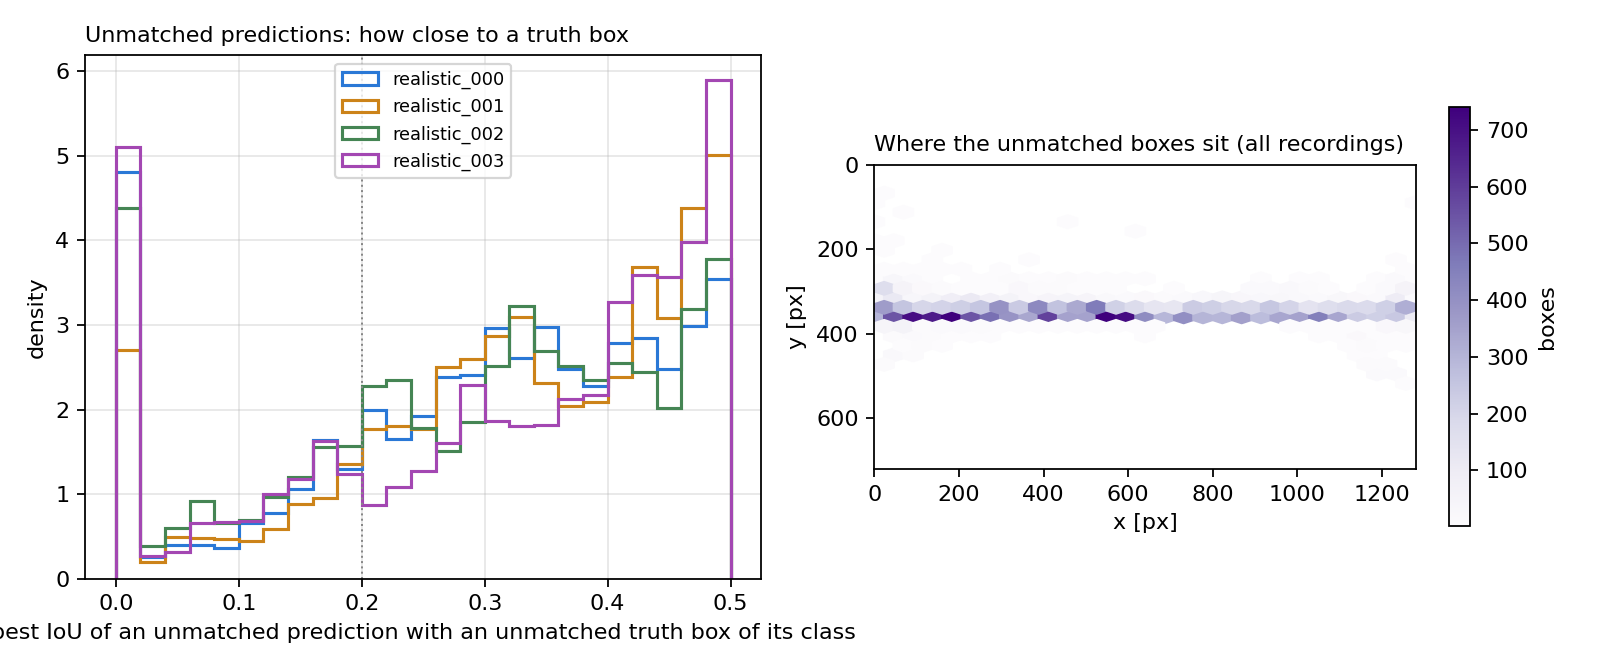
\includegraphics[width=\textwidth]{figures/yolo_fig_fp_anatomy.png}
  \caption[What the unmatched predictions are.]{What the unmatched predictions
  are, per recording: near misses
  (right object, IoU 0.2--0.5), slight overlaps, boxes on nothing, and
  predictions ignored on unlabelled scenery.}
  \label{fig:exp2-fp}
\end{figure}

\textbf{Limitations, each stated once.} \emph{Projected truth:} boxes are the
projection of collision meshes, tighter than a human would draw and exempted
by rules a human would not apply; the scored basis is the easier one and both
are given. \emph{People:} the walking people are actors without pose or mesh
and outside the checkpoint's classes; no truth exists for them, their
detections (if any) are charged as false positives, and a filter built on
this detector cannot mask them at all. \emph{One operating point:} a single
confidence threshold was retained, so no average precision. \emph{Checkpoint
provenance:} the four-class checkpoint was trained on 8 October 2026 and its
training set is not registered in this write-up.

\paragraph{Summary.} The detector is reliable at naming and unreliable at
finding: class F1 0.994 given a match, recall 0.50 over the boxes it is
asked to find and 0.29 over everything in view, moving-object recall 0.29.
The miss is a size effect and the false positives are mostly boxes a little
off the right object. For the filters of Experiment~3 the input is a mask
that covers under a third of the moving pallet jacks' frames and none of the
people.

\paragraph{Future plan.} Add a person class and give the actors projectable
geometry, or annotate a frame subset by hand, so that the moving agents the
filter exists for are all scorable; raise the input resolution or the
training set's share of small boxes, since the miss is a size effect; and
report a precision--recall curve from a run with the threshold at zero.

\FloatBarrier

\FloatBarrier
\subsection{Real robot}
\label{sec:exp2-real}

\slotstatus{planned}{Real imagery exists; no real ground-truth boxes do.}

\textbf{Reason.} Projected ground truth needs object poses and meshes,
which the real site does not provide. The four real recordings in use
(\repo{realv6_000}, \repo{realv7_000}--\repo{002}) hold the imagery, so the
detector can be run on them, but nothing can score it until frames are
annotated by hand.

\textbf{Next action.} Annotate a stratified frame subset of
\repo{dataset_realv6_000} and \repo{dataset_realv7_000} to \repo{_002} across
the illumination levels of the test site, run the detector at confidence 0.35
and matching IoU 0.5, and report precision, recall, F1 and moving-object
recall; the same annotated subset is the only route to a scored simulation
slot as well, since the realistic worlds give the detector nothing projectable
to find.

% =====================================================================
\FloatBarrier
\section{Experiment 3: Dense Map Reconstruction and Map-Quality Evaluation}
\label{sec:exp3}

\FloatBarrier
\subsection{Simulation}
\label{sec:map-quality}

\slotstatus{partial}{Five databases are scored for geometry and drivability:
the tiny warehouse, which passes, and four realistic-warehouse maps --- two
mapping recordings, one per layout, each built closure-free under two
back-end configurations, A and B --- all of which fail the quality
criterion fixed before scoring. The tiny map's independent drivability
reference remains lost.}

\textbf{Objective.} Verify that the reconstructed map reflects the physical
environment and is usable by a planner (\cref{sec:map-eval-method}).

\textbf{Process.} RTAB-Map 0.23.7 built \repo{map/map_tiny.db}; its placement
was measured by \repo{script/fit_map_pose.py}; geometry and drivability were
scored by \repo{script/validate_map.py} against the world file and a
ground-truth route. Four further databases were built in the realistic worlds
with loop closure disabled on both sides of the pipeline, two per layout under
the October and the current configuration, and scored by the same two scripts,
each against a recording that did not build it (\cref{sec:map-realistic}).

\textbf{Dataset.} \repo{dataset_map_tiny} (the build run) and the independent
route \repo{dataset_static_tiny_repeat}, which no longer exists; and, for the
large warehouse, \repo{dataset_map_01} (\cref{tab:dataset-registry}). The
realistic-warehouse builds postdate that registry:
\repo{dataset_allsensor_realistic_map} (U layout, \SI{285.7}{\second}; held
until 26 October as \repo{_mapv2}) built \repo{map/map_realistic} and
\repo{map/dataset_allsensor_realistic_map}, and
\repo{dataset_allsensor_realistic_01_map} (I layout, \SI{314.9}{\second})
built \repo{map/map_realistic_01} and
\repo{map/dataset_allsensor_realistic_01_map}; their independent probes are
the static twins \repo{dataset_allsensor_realistic_000} and \repo{_001} of
\cref{sec:realistic-worlds}.

% Verbatim from minor_report/chapters/chapter_4_results.tex lines 1399-1707 (retired report),
% headings demoted by 1 level(s). Do not edit here; edit the source of the numbers.

\subsubsection{Question, scope, and conditions}

Trajectory error answers whether the robot knew where it was. It does not answer
whether the map it produced describes the building, nor whether a planner could
have used that map. This section evaluates the one dense map reconstructed so far
against two references of very different strength: the simulator's own collision
geometry, which is independent of the map, and the ground-truth route of the run
that built the map, which is not. The two questions are kept separate because
they fail in different ways --- a map can be geometrically faithful and still
unusable, and it can be navigable over an easy route while misrepresenting the
parts of the building that route never entered --- and because only the first
reference is independent evidence.

The evaluation is confined to the \textbf{tiny} warehouse. A large-warehouse
equivalent is \status{planned}; no database for it exists at the reporting
cutoff. Tiny-map and large-map results must not be pooled or read as repeated
trials of one condition, because the two worlds differ in extent, aisle width,
and route length. \Cref{tab:map-conditions} records the conditions.

\begin{table}[htbp]
\centering
\caption[Conditions for the dense-map evaluation.]{Conditions for the dense-map evaluation. The database and the
ground-truth route come from the \emph{same} run, which bounds what the
drivability figures can establish.}
\label{tab:map-conditions}
\small
\begin{tabularx}{\textwidth}{>{\raggedright\arraybackslash}p{0.26\textwidth}>{\raggedright\arraybackslash}X}
\toprule
Factor & Level \\
\midrule
Map under test & \repo{map/map_tiny.db}, RTAB-Map 0.23.7, created 2026-09-08 \\
World &
  \repo{aws-robomaker-small-warehouse-world/worlds/small_warehouse_static/small_warehouse_static_tinymap.world}
  (tiny geometry, despite residing in the \repo{small_warehouse_static} family
  directory) \\
Scene dynamics & static \\
Grid resolution & \SI{0.05}{\metre} \\
Geometry tolerance & \SI{0.25}{\metre} \\
Robot footprint & $0.83\times0.50$~m rectangle from
  \repo{nav2_ackermann.yaml}, not a circumscribed radius \\
World-to-map placement & $x=\SI{1.850}{\metre}$, $y=\SI{8.600}{\metre}$,
  $\theta=\SI{-89.90}{\degree}$, measured once by \repo{script/fit_map_pose.py} \\
Drivability reference, as plotted & \repo{dataset_static_tiny_repeat},
  \num{2973} poses; an independent run, no longer present in the workspace or on
  the removable drive \\
Substitute available & \repo{dataset/dataset_map_tiny},
  \repo{/ground_truth/odometry}: \num{3032} messages over \SI{60.6}{\second} of
  simulation time. This is the run that \emph{built} the map, so it is not an
  equivalent replacement \\
Evaluator & \repo{script/validate_map.py} \\
Experimental unit, $n$ & one database; $n=1$ \\
\bottomrule
\end{tabularx}
\end{table}

\subsubsection{Map placement as a validity precondition}
\label{sec:map-placement}

Both metrics depend on seating the occupancy grid in world coordinates, so
placement is a precondition rather than a display choice: a mis-seated grid
scores real structure against the wrong cells and makes a good map look bad. The
transform is a constant for a given database and is measured once, by fitting
occupied cells to the world file's wall and obstacle edges without using odometry
or ground truth. It is deliberately not taken from the live
\texttt{map~$\rightarrow$~odom} correction, which moves with front-end drift.

The measured fit is $(1.850, 8.600)\,\si{\metre}$ at \SI{-89.90}{\degree}, with a
margin of \SI{60.9}{\percent} over the best rival orientation more than
\SI{5}{\degree} away. An independent prediction --- the spawn pose of the IMU body
frame, which sits \SI{0.338}{\metre} ahead of \texttt{base\_footprint} --- gives
$(1.800, 8.662)\,\si{\metre}$. The two agree to \SI{0.080}{\metre}, inside the
grid's own \SI{0.05}{\metre} resolution. Two independent routes to the same
number is what makes this a measurement rather than a tuned parameter.

\subsubsection{Graph and database summary}

\Cref{tab:map-graph} summarizes the stored graph, read directly from the database
in read-only mode. The counts are small: \num{30} nodes over a \SI{59.3}{\second}
span, reflecting RTAB-Map's retention policy rather than the rate at which images
were offered to it.

\begin{table}[htbp]
\centering
\caption[Stored contents of \repo{map/map_tiny.db}.]{Stored contents of \repo{map/map_tiny.db}. Link rows are stored per
direction; the undirected count is the number of distinct node pairs.}
\label{tab:map-graph}
\small
\begin{tabularx}{\textwidth}{>{\raggedright\arraybackslash}p{0.30\textwidth}rr>{\raggedright\arraybackslash}X}
\toprule
Element & Rows & Undirected & Note \\
\midrule
Nodes & 30 & -- & ids 1--30, stamp span \SI{59.3}{\second} \\
Neighbour links & 56 & 28 & sequential odometry constraints \\
Global loop closures & 5 & 3 & pairs $(9,22)$, $(10,23)$, $(29,30)$ \\
Gravity links & 30 & 30 & one per node \\
Local-space links & 0 & 0 & none recorded \\
Visual words & \num{10357} & -- & vocabulary size \\
Features & \num{28374} & -- & stored keypoints \\
\bottomrule
\end{tabularx}
\end{table}

Of the three distinct closure pairs, $(9,22)$ and $(10,23)$ join nodes roughly
half a lap apart and are genuine revisits of an earlier place. The third,
$(29,30)$, joins consecutive nodes and is therefore not a revisit; it should not
be counted as evidence of place recognition.

\subsubsection{Geometry against the world file}

Geometry is scored against the rasterized collision geometry of the world file at
a \SI{0.25}{\metre} tolerance. Recall is measured against \emph{surfaces} rather
than filled interiors, because a stereo camera can only observe the outside of a
shelf; counting its interior as missed geometry would cap even a perfect map well
below \SI{100}{\percent}.

\begin{table}[htbp]
\centering
\caption{Occupied-cell geometry of \repo{map/map_tiny.db} against
\repo{small_warehouse_static_tinymap.world} at \SI{0.25}{\metre} tolerance.}
\label{tab:map-geometry}
\small
\begin{tabularx}{\textwidth}{>{\raggedright\arraybackslash}p{0.34\textwidth}r>{\raggedright\arraybackslash}X}
\toprule
Metric & Value & Population \\
\midrule
Occupied-cell precision & \SI{96.6}{\percent} & \num{11634} occupied cells \\
Recall, region the map observed & \SI{89.5}{\percent} & observed surfaces \\
Recall, whole building & \SI{67.2}{\percent} & all surfaces in the world file \\
\bottomrule
\end{tabularx}
\end{table}

The gap between \SI{89.5}{\percent} and \SI{67.2}{\percent} is route coverage, not
mapping failure: the run never entered the side aisles, so roughly a third of the
building was never observed by any sensor. The two numbers answer different
questions and neither replaces the other --- the first is a statement about
mapping quality, the second about where the robot went.

\subsubsection{Drivability against the true route}
\label{sec:map-drivability}

The robot demonstrably drove the reference route, so every pose on it was
collision-free in reality. Stamping the real footprint onto the map at each pose
therefore converts any collision into a \emph{proven} false obstacle, and any
unknown cell into a hole a planner would have to cross blind. This metric needs no
assumption about what a good map looks like.

It does, however, depend on where the route came from, and that is the weak point
of this result. The route used to produce \cref{tab:map-drivability} came from a
separate run, \repo{dataset_static_tiny_repeat}, which is no longer present in
the workspace or on the removable drive. The figures below therefore stand as a
dated independent measurement that cannot currently be re-derived.

The only surviving recording of this warehouse, \repo{dataset/dataset_map_tiny},
is not an equivalent substitute, because it is the run that built the map. Three
measurements establish this. Applying the placement of
\cref{sec:map-placement} to the stored node poses puts them a median of
\SI{0.069}{\metre} from that recording's ground-truth route; comparing each node
against the ground-truth pose carrying the \emph{same} timestamp gives a median
of \SI{0.340}{\metre} and a maximum of \SI{0.52}{\metre}; and all \num{30}
nodes fall inside the recording's sim-time interval. The second of these is the
discriminating one, since a different run over the same loop would agree in space
but not in time. The two routes are also visibly different: the lost run is a
single oval circuit, while this one is a figure-eight through the centre of the
building.

The evaluation was nevertheless repeated against this recording, and the outcome
confirms the objection rather than resolving it. Both results are reported in
\cref{tab:map-drivability}.

\begin{table}[htbp]
\centering
\caption[Drivability of \repo{map/map_tiny.db} under the true $0.83\times0.50$~m nav2 footprint, evaluated against two different routes.]{Drivability of \repo{map/map_tiny.db} under the true
$0.83\times0.50$~m nav2 footprint, evaluated against two different routes.
``Independent'' is \repo{dataset_static_tiny_repeat}, the run that did not build
the map and is no longer available. ``Build run'' is
\repo{dataset/dataset_map_tiny}, the run the map was constructed from. Geometry
is identical in both cases because it does not depend on the route.}
\label{tab:map-drivability}
\small
\setlength{\tabcolsep}{4pt}
\begin{tabularx}{\textwidth}{>{\raggedright\arraybackslash}p{0.30\textwidth}rr>{\raggedright\arraybackslash}X}
\toprule
Metric & Independent & Build run & Meaning \\
\midrule
Poses scored & \num{2973} & \num{3032} & \\
Clear and mapped & \SI{99.3}{\percent} & \SI{100.0}{\percent} & footprint free
  and observed \\
False obstacle & \SI{0.7}{\percent} & \SI{0.0}{\percent} & proven error \\
Unmapped under footprint & \SI{0.0}{\percent} & \SI{0.0}{\percent} & blind cells
  on the route \\
Clearance, median & \SI{1.07}{\metre} & \SI{1.01}{\metre} & to nearest obstacle \\
Clearance, 5th percentile & \SI{0.45}{\metre} & \SI{0.46}{\metre} & inflation
  radius is \SI{0.80}{\metre} \\
\bottomrule
\end{tabularx}
\end{table}

The difference between the two columns is the independence effect, measured rather
than assumed. Against the run that built it, the map records \emph{no} false
obstacle at all: it cannot contradict the trajectory it was constructed from. The
\SI{0.7}{\percent} that the independent run exposes is precisely the part of the
map that only a route the mapper had not seen could reveal. The right-hand column
is therefore not a better result than the left; it is a weaker question, and the
\SI{0.0}{\percent} should not be quoted as a map-quality figure.

Clearance is nearly unchanged between the two, which is expected: it is a property
of where each route runs relative to mapped geometry, not of which run built the
map. Both routes spend part of their length inside nav2's inflation radius.

\begin{figure}[htbp]
  \centering
  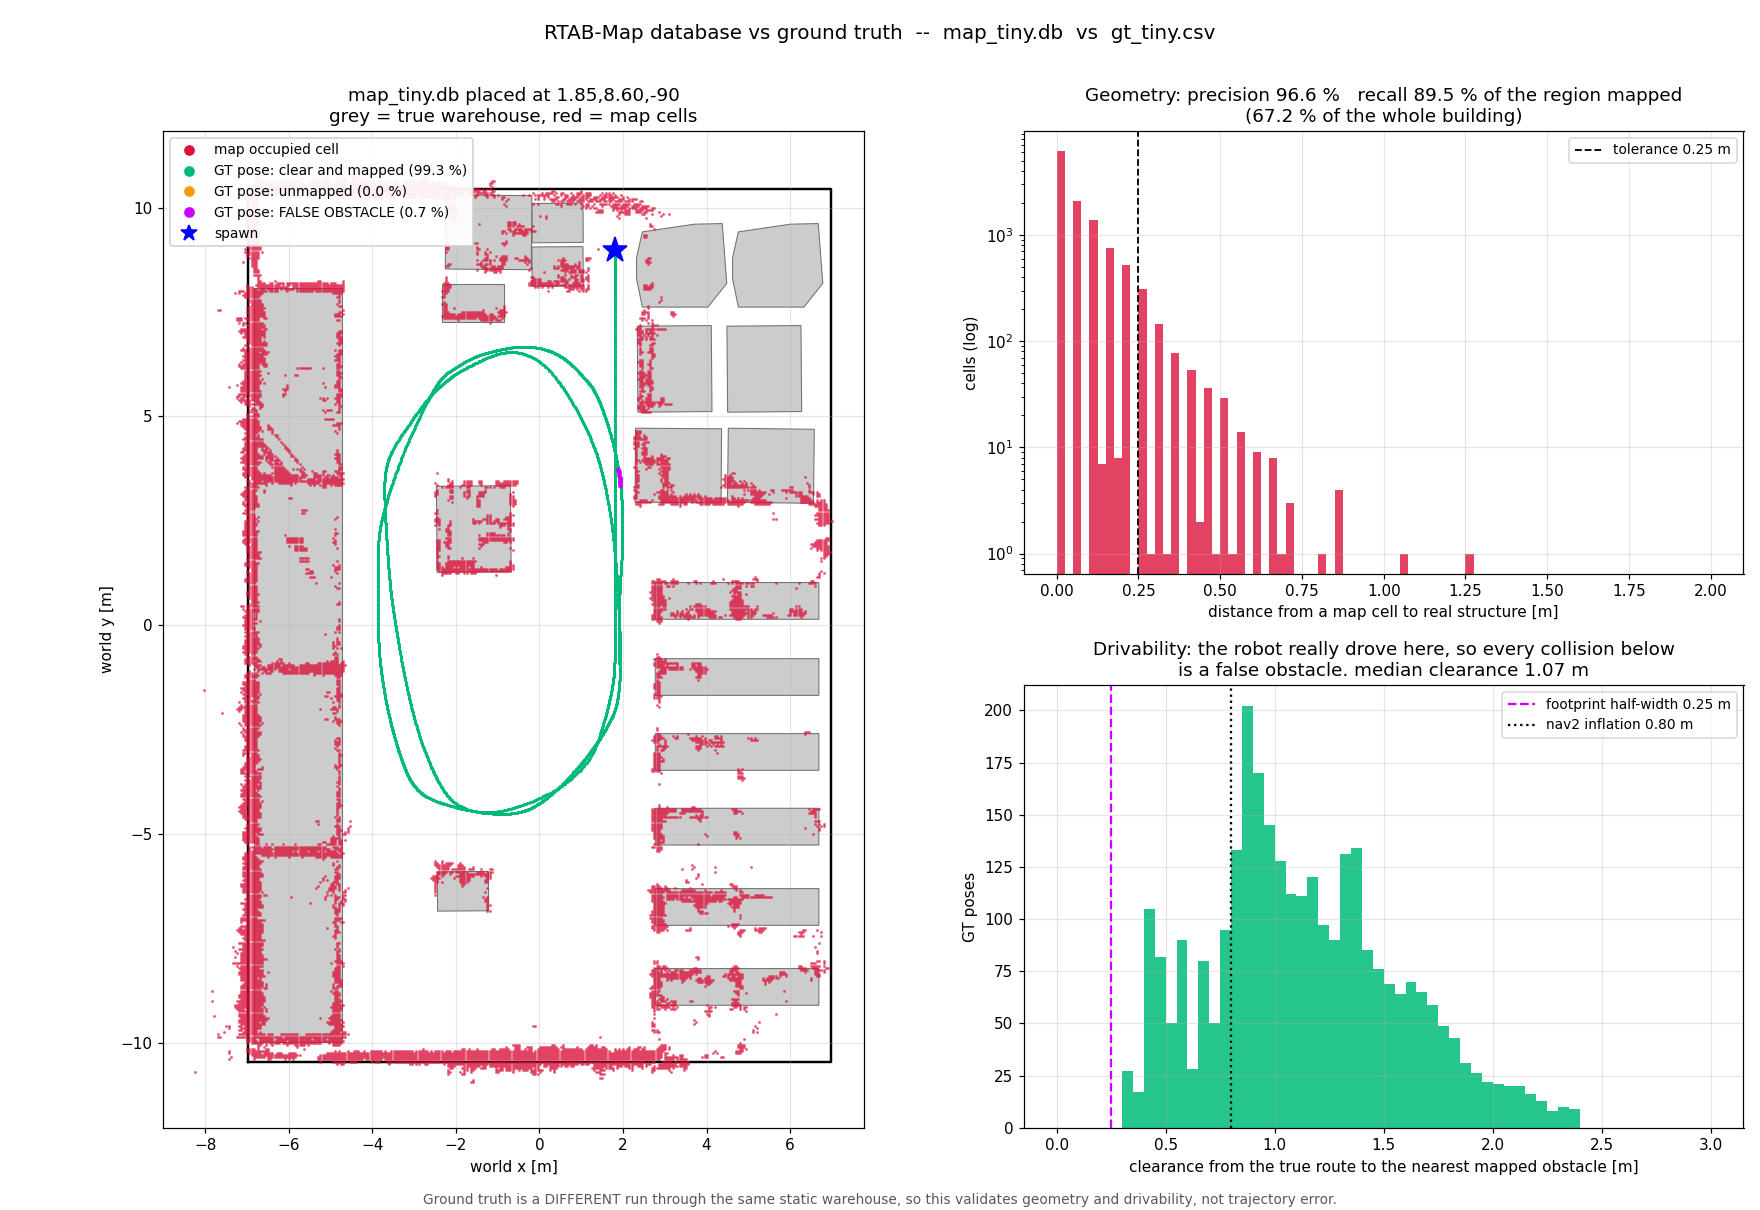
\includegraphics[width=\textwidth]{../../../output/compare/rtab_map_vs_gt.png}
  \caption[Dense-map evaluation of \repo{map/map_tiny.db}.]{Dense-map evaluation of \repo{map/map_tiny.db}. Left: occupied cells
  (red) over the world file's true collision geometry (grey), with the
  ground-truth route coloured by drivability and the spawn marked. Top right:
  distance from each occupied cell to real structure, with the
  \SI{0.25}{\metre} tolerance marked; the bulk falls well inside tolerance with a
  thin tail to about \SI{1.25}{\metre}. Bottom right: clearance from the true
  route to the nearest mapped obstacle, against the footprint half-width and the
  nav2 inflation radius. The ground truth was a different run through the same
  static warehouse, so this validates geometry and drivability, not trajectory
  error; that run is no longer available
  (\cref{sec:map-drivability}).}
  \label{fig:map-vs-gt}
\end{figure}

\begin{figure}[htbp]
  \centering
  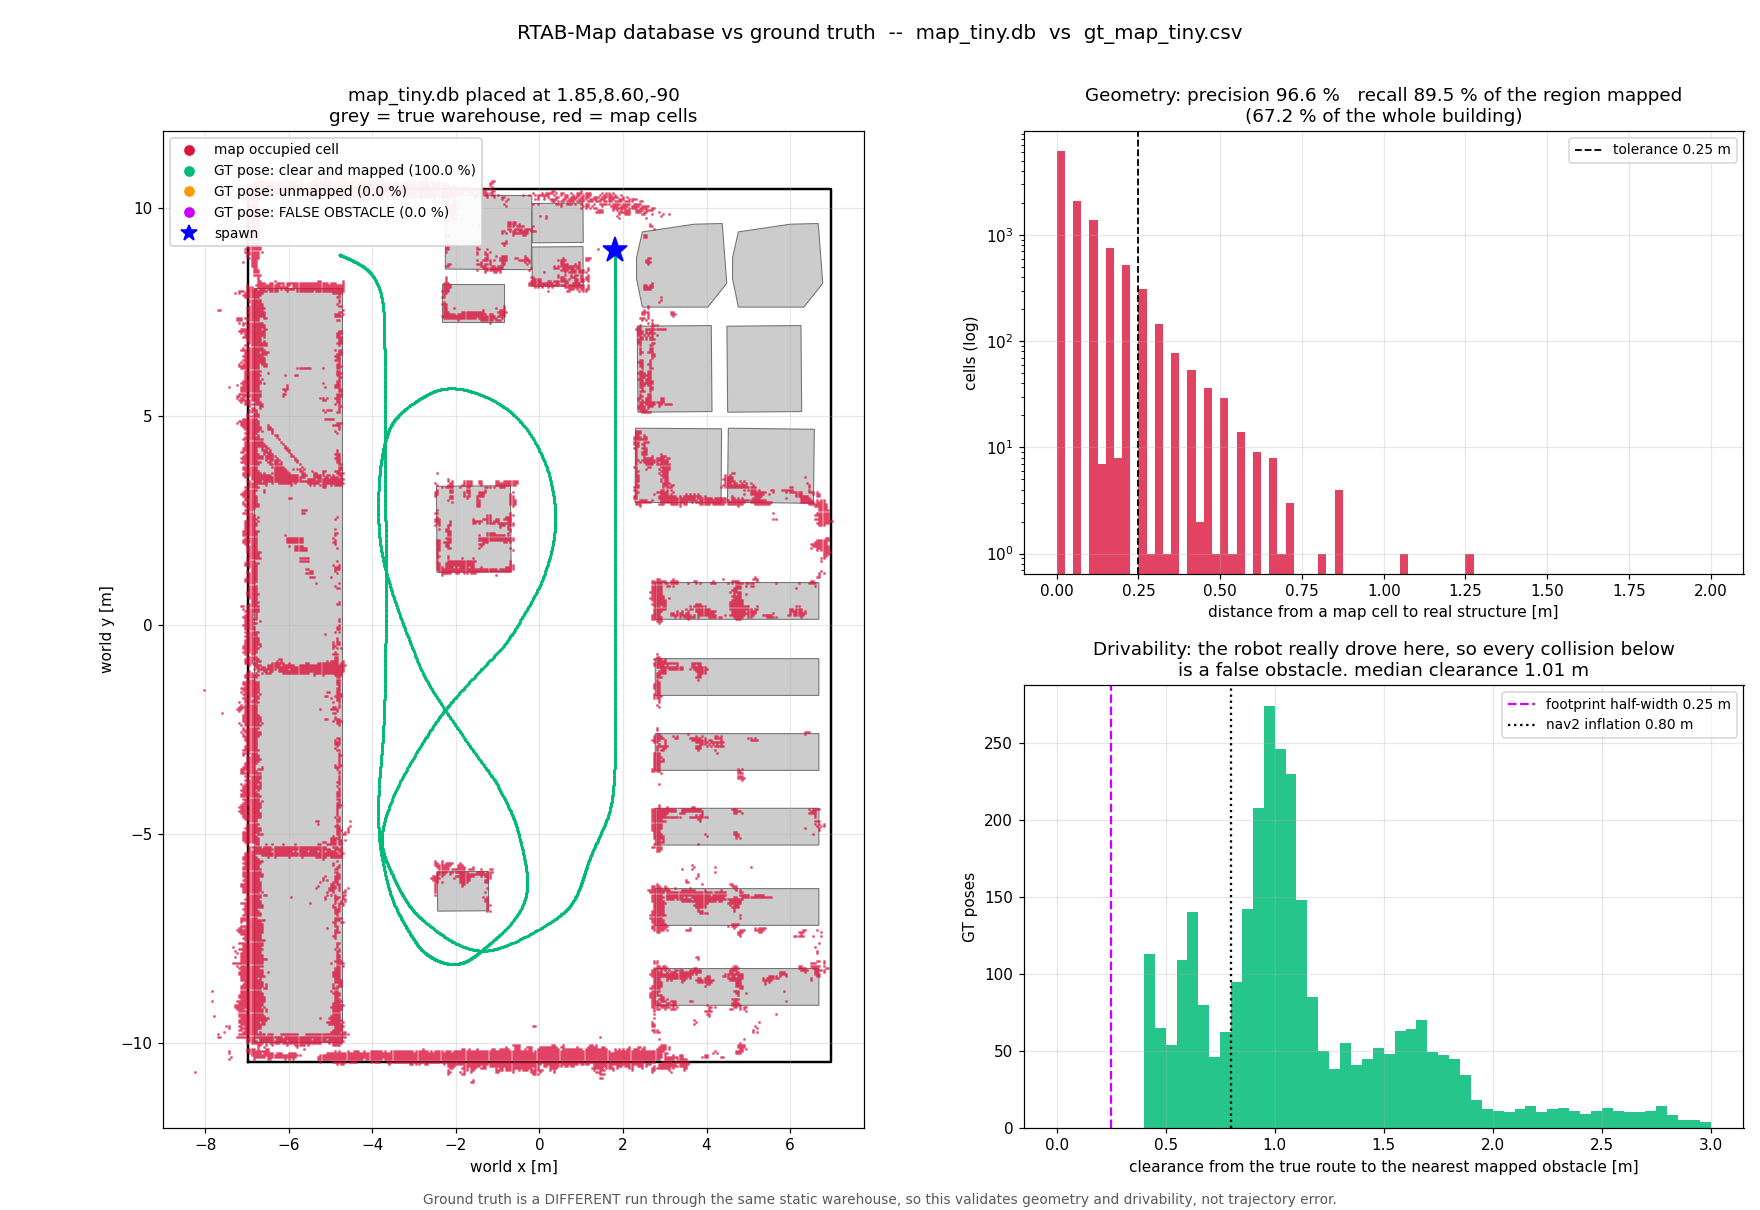
\includegraphics[width=\textwidth]{../../../output/compare/rtab_map_vs_gt_selfcheck.png}
  \caption[The same database scored against the run that built it, \repo{dataset/dataset_map_tiny}.]{The same database scored against the run that built it,
  \repo{dataset/dataset_map_tiny}. The route is a figure-eight rather than the
  oval of \cref{fig:map-vs-gt}, and no pose on it collides with the map: the
  false-obstacle rate falls from \SI{0.7}{\percent} to \SI{0.0}{\percent}. The
  geometry panels are identical to \cref{fig:map-vs-gt} because geometry does not
  depend on the route. The footer claiming a different run is emitted
  unconditionally by the evaluator and is incorrect for this figure.}
  \label{fig:map-vs-gt-selfcheck}
\end{figure}

\subsubsection{Interpretation and limitations}

Within its stated scope the tiny map is geometrically faithful and navigable:
\SI{96.6}{\percent} of what it marks as occupied is real, it recovers
\SI{89.5}{\percent} of the surfaces it actually observed, and it contains no blind
cells and only \SI{0.7}{\percent} proven false obstacles along a route the robot
really drove. The geometry half of that is independent evidence and is the
strongest map result the project currently holds; the drivability half is a
self-consistency check and is weaker than it looks. Both are a direct improvement
on earlier assessments that judged the same database unnavigable --- those were measured with the grid mis-seated, so the comparison
was against the wrong cells. That correction is a methodological finding in its
own right and is why \cref{sec:map-quality} reports placement before any metric.

Four limitations bound what these numbers support.

\begin{itemize}
  \item \textbf{The drivability reference cannot be re-read.} The run that
    provided it is lost, and the only surviving recording of this warehouse is the
    one that built the map, which would answer a weaker question. Re-establishing
    this result needs a fresh independent recording --- a second run, not a second
    map.
  \item \textbf{The route is easy.} It is one large loop down the wide central
    aisle and never squeezes into a side aisle. The \SI{0.7}{\percent} false-obstacle
    figure is therefore a floor, not a worst case. A route through the narrow
    aisles is the test that would actually stress this map, and it has not been
    run.
  \item \textbf{Clearance couples to planner cost.} The 5th-percentile clearance
    of \SI{0.45}{\metre} sits below nav2's \SI{0.80}{\metre} inflation radius, and
    a visible share of the true route lies inside it. Nothing is blocked, but a
    planner would charge a high cost for driving where the robot demonstrably
    drove. That coupling should be examined before any planned path is trusted.
  \item \textbf{$n=1$, and the scope is one world.} A single database on the tiny
    warehouse supports no uncertainty estimate and no claim about the large
    warehouse, where longer routes and narrower bays change both the drift
    exposure and the clearance margin.
  \item \textbf{Residual distortion is not a placement problem.} Walls appear
    doubled and thickened and shelf rows bowed in the overlay. No rigid transform
    removes that; it is internal map distortion and is the property that would
    limit navigation, independently of how well the grid is seated.
\end{itemize}

\begin{queried}[Queried: reproducibility of the drivability half]
The geometry result is fully reproducible: both \repo{map/map_tiny.db} and the
world file are present. The drivability result is not. Its reference run,
\repo{dataset_static_tiny_repeat}, is absent from \repo{dataset/} and from the
removable drive, and the only surviving recording of this warehouse is the one
that built the map, which would answer a weaker question
(\cref{sec:map-drivability}). The database additionally stores an empty parameter
set, so the configuration that produced it is not recoverable from the file, and
the RTAB-Map engineering record's claim that the node stamps match no dataset is
contradicted by the pose agreement reported above. The drivability figures should
therefore be read as a dated measurement rather than a standing result, and should
not be carried into the major report until an independent route has been recorded
and retained.
\end{queried}

\subsubsection{Planned extension to the large warehouse}

The same evaluation is \status{planned} for the large warehouse and is not
started: no large-map database exists at the cutoff. Three things must be settled
before those numbers would mean anything. The world-to-map placement must be
measured for the new database rather than assumed, since the tiny-map constant
$(1.850, 8.600, \SI{-89.90}{\degree})$ is specific to that database and world. A
ground-truth route must be recorded from a run \emph{other} than the one that
builds the map, which the tiny-map case did not do and which is what would turn
drivability into independent evidence. Finally, the route should deliberately
include narrow bays, so that the false-obstacle rate is exercised rather than
merely reported. Until then,
no map-quality claim extends beyond the tiny warehouse.


\subsubsection{Large-warehouse attempt}
\label{sec:map-large}

The progress update of 23 September 2026 reports that the large-warehouse map
attempt \status{failed}: the front end lost tracking in the repetitive bay
structure of the large world, the estimated pose diverged from the ground-truth
route within a few time steps of the loss, and the resulting map was not
scorable. The failure was attributed there to the front end under repeated
structure, not to the mapping back end.
\flag{No database, run directory or figure for this attempt is registered in
the repository at the cutoff, so the result is reported on the strength of the
progress record and cannot be audited. A database identified from its contents
as this attempt (18 nodes, \SI{37}{\metre} along one aisle, poses leaving the
floor, placeable in no large world) was found among the unregistered
databases on 22 October 2026 and deleted with them on 6 November, unscored.
The attempt must be repeated with its artifacts retained before it is carried
into any conclusion.}

\subsubsection{Realistic-warehouse maps}
\label{sec:map-realistic}

Four databases built in the realistic
worlds of \cref{sec:realistic-worlds} replace the unauditable large-warehouse attempt: two
mapping recordings, one per layout, each built twice, under two back-end configurations, A and B. Every one has a
registered build recording, a fitted placement, a score and a figure, and all
four fail the quality criterion fixed before they were scored.

\textbf{Reporting rules.} The criterion, fixed in
\repo{script/eval_realistic_maps.py} before any map was placed, is occupied-cell
precision $\ge$ \SI{90}{\percent}, observed-region recall $\ge$ \SI{85}{\percent}
and false obstacles $\le$ \SI{1}{\percent} of probe poses, each taken from the
tiny map's result; whole-building recall is reported, not tested. The metrics
are those of \cref{sec:map-eval-method}. Placement was
measured by \repo{script/fit_map_pose.py} with the realistic spawn
$(5.250, 19.995, \SI{-90}{\degree})$ and confirmed on the overlays before
scoring. Scoring is the unchanged \repo{script/validate_map.py} at
\SI{0.25}{\metre} tolerance with the $0.83\times0.50$~m footprint, each map
probed by the static twin of its own layout, a recording that built none of
them. All four databases are closure-free (\repo{Rtabmap/LoopThr} 1.0,
\repo{RGBD/ProximityBySpace} false; \repo{loop_closure:=false}, RTAB-Map record
\S7c) and optimised with GTSAM. The two builds of each recording differ in
exactly three back-end parameters, \repo{Rtabmap/DetectionRate} 4 against
\SI{1}{\hertz}, \repo{Grid/RangeMax} 8 against \SI{10}{\metre} and
\repo{Grid/MaxGroundHeight} 0.29 against \SI{0.10}{\metre} (build A against build B), and in front-end session, which neither database records; they are
two configurations, not a repeat pair, so $n=1$ per cell and no difference
between builds is attributable to one parameter. The recording now named
\repo{dataset_allsensor_realistic_map} is the one held until 26 October as
\repo{_mapv2} (identical message counts); the original 103--316\,s mapping
recording and the 114-node database built from it were deleted that day, and
\repo{map/map_realistic} is the former \repo{map_realistic_v2}. Node stamps fix
the pairing: the U databases span 13--300\,s and the I databases 20--335\,s,
which the 125\,s and 97\,s probes cannot have produced. The November U
placement was fitted in the \SI{-180}{\degree} basin with \repo{--yaw-near},
because the global winner, \SI{4.2}{\percent} better by agreement, was the
rotational rival the overlay rejects; both candidates are in
\repo{fit_dataset_allsensor_realistic_map.log}. Every number is under the
experiment directory \repo{exp4-realistic-maps} of
\repo{output/compare/simulation}: the scores in
\repo{realistic_map_metrics.csv}, one \repo{validate_*.json} per map, the
inventory with the three parameters in \repo{map_inventory.json}, and the
placement logs.

\textbf{Results.} \Cref{tab:map-realistic-geometry} gives geometry,
\cref{tab:map-realistic-drivability} drivability against the independent
probes, \cref{tab:map-graph-accuracy} the accuracy of the graph each map was
built from, and \cref{tab:map-realistic-graph} the stored graphs and the three
parameters that separate the builds.
\Cref{fig:map-realistic-fit,fig:map-realistic-nov-fit} are the placement
overlays of the two U builds and
\cref{fig:map-realistic-validate,fig:map-realistic-nov-validate,fig:map-realistic-01-validate,fig:map-realistic-01-nov-validate}
the evaluation overlays.

\begin{table}[htbp]
\centering
\caption[Occupied-cell geometry of the four realistic databases.]{Occupied-cell
geometry of the four realistic-warehouse databases
against their world files at \SI{0.25}{\metre} tolerance, beside the tiny map.
Bold marks a value below the fixed criterion.}
\label{tab:map-realistic-geometry}
\small
\setlength{\tabcolsep}{4pt}
\resizebox{\textwidth}{!}{%
\begin{tabular}{llrrrrr}
\toprule
Database & Config.\ & Nodes & Occupied & Precision & Recall & Recall \\
 & & & cells & & observed & building \\
 & & & & [\si{\percent}] & [\si{\percent}] & [\si{\percent}] \\
\midrule
\repo{map_tiny} & --- & 30 & 11\,634 & 96.6 & 89.5 & 67.2 \\
\repo{map_realistic} & A & 165 & 26728 & \textbf{81.2} & \textbf{82.5} & 55.7 \\
\repo{dataset_allsensor_realistic_map} & B & 148 & 22715 & \textbf{77.8} & \textbf{74.9} & 57.1 \\
\repo{map_realistic_01} & A & 185 & 25440 & \textbf{84.8} & \textbf{81.4} & 54.5 \\
\repo{dataset_allsensor_realistic_01_map} & B & 127 & 23255 & \textbf{82.2} & \textbf{77.1} & 55.3 \\
\bottomrule
\end{tabular}}
\end{table}

\begin{table}[htbp]
\centering
\caption[Drivability of the realistic-warehouse databases.]{Drivability of the four
realistic-warehouse databases under the true $0.83\times0.50$~m nav2
footprint, against the independent probe of each layout; U-A is
\repo{map_realistic}, U-B \repo{dataset_allsensor_realistic_map}, I-A
\repo{map_realistic_01}, I-B \repo{dataset_allsensor_realistic_01_map}. The
tiny map's independent figures were 2\,973 poses, \SI{0.7}{\percent} false
obstacles, clearance 1.07 and \SI{0.45}{\metre}; its probe was one loop of a
wide aisle, so the comparison is not route-matched.}
\label{tab:map-realistic-drivability}
\footnotesize
\setlength{\tabcolsep}{4pt}
\begin{tabular}{lrrrr}
\toprule
Metric & U-A & U-B & I-A & I-B \\
\midrule
Probe poses & 6278 & 6278 & 4847 & 4847 \\
Clear and mapped [\si{\percent}] & 96.2 & 95.0 & 94.9 & 89.5 \\
False obstacle [\si{\percent}] & \textbf{3.8} & \textbf{5.0} & \textbf{4.4} & \textbf{10.2} \\
Unmapped under footprint [\si{\percent}] & 2.4 & 1.9 & 0.7 & 0.5 \\
Clearance, median [\si{\metre}] & 1.96 & 2.00 & 2.16 & 1.98 \\
Clearance, 5th percentile [\si{\metre}] & 0.62 & 0.38 & 0.36 & 0.18 \\
\bottomrule
\end{tabular}
\end{table}

\begin{table}[htbp]
\centering
\caption[Stored contents and build parameters of the realistic-warehouse
databases.]{Stored contents and build parameters of the four
realistic-warehouse databases, read in read-only mode. The three parameter rows
are the only ones that differ between the builds of a recording. Neighbour
links are stored per direction; a ``spanning'' closure joins nodes more than
three apart and none exists, by configuration. The margin is the agreement
over the best rival more than \SI{5}{\degree} away; ``basin'' marks the
placement chosen with \repo{--yaw-near}.}
\label{tab:map-realistic-graph}
\scriptsize
\setlength{\tabcolsep}{3pt}
\resizebox{\textwidth}{!}{%
\begin{tabular}{lrrrr}
\toprule
 & U-A & U-B & I-A & I-B \\
\midrule
\repo{Rtabmap/DetectionRate} [\si{\hertz}] & 4.0 & 1.0 & 4.0 & 1.0 \\
\repo{Grid/RangeMax} [\si{\metre}] & 8.0 & 10.0 & 8.0 & 10.0 \\
\repo{Grid/MaxGroundHeight} [\si{\metre}] & 0.29 & 0.1 & 0.29 & 0.1 \\
Nodes & 165 & 148 & 185 & 127 \\
Node stamp span [\si{\second}] & 285.7 & 286.2 & 314.9 & 313.9 \\
Optimised path [\si{\metre}] & 369.5 & 364.2 & 384.7 & 372.3 \\
Neighbour links, rows & 322 & 294 & 356 & 248 \\
Closure rows / spanning $>3$ & 3 / 0 & 0 / 0 & 4 / 0 & 0 / 0 \\
Visual words & 55802 & 51539 & 63276 & 44342 \\
Database size [\si{\mega\byte}] & 417 & 462 & 438 & 377 \\
Placement $(x,y,\theta)$ & $(5.300, 19.500, \SI{-179.9}{\degree})$ & $(5.200, 19.800, \SI{-180.1}{\degree})$ & $(5.150, 20.450, \SI{179.4}{\degree})$ & $(4.950, 20.400, \SI{-179.9}{\degree})$ \\
Fit agreement, margin & 0.183, \SI{+10.1}{\percent} & 0.161, \SI{-4.2}{\percent} (basin) & 0.260, \SI{+66.1}{\percent} & 0.252, \SI{+60.2}{\percent} \\
\bottomrule
\end{tabular}}
\end{table}

\begin{figure}[p]
  \centering
  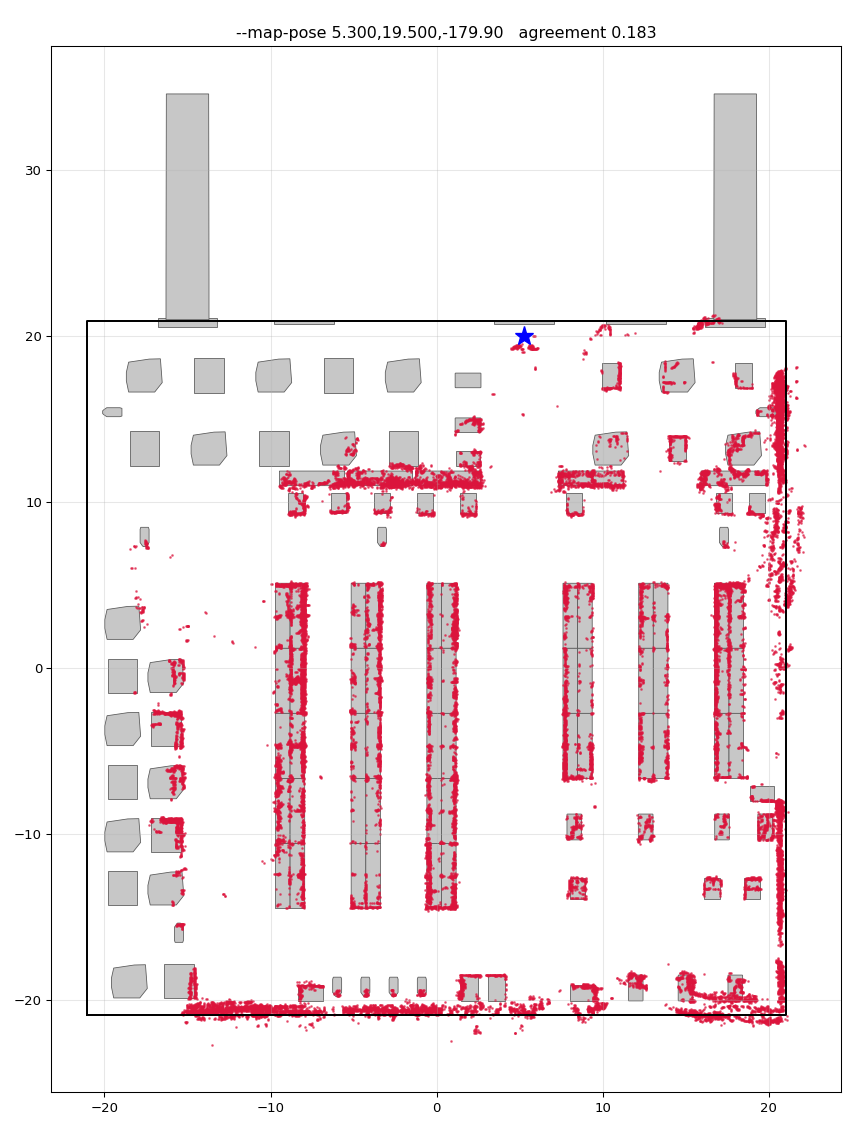
\includegraphics[width=0.7\textwidth]{figures/map_realistic_fit.png}
  \caption[Placement overlay of \repo{map/map_realistic} (U-A).]{Placement
  overlay of \repo{map/map_realistic} (U-A), agreement 0.183,
  \SI{10.1}{\percent} margin over the rival orientation. Red occupied cells
  over the world file's obstacle footprints and wall; shelf rows, the bay strip
  at $y\approx11$ and all four walls coincide.}
  \label{fig:map-realistic-fit}
\end{figure}

\begin{figure}[p]
  \centering
  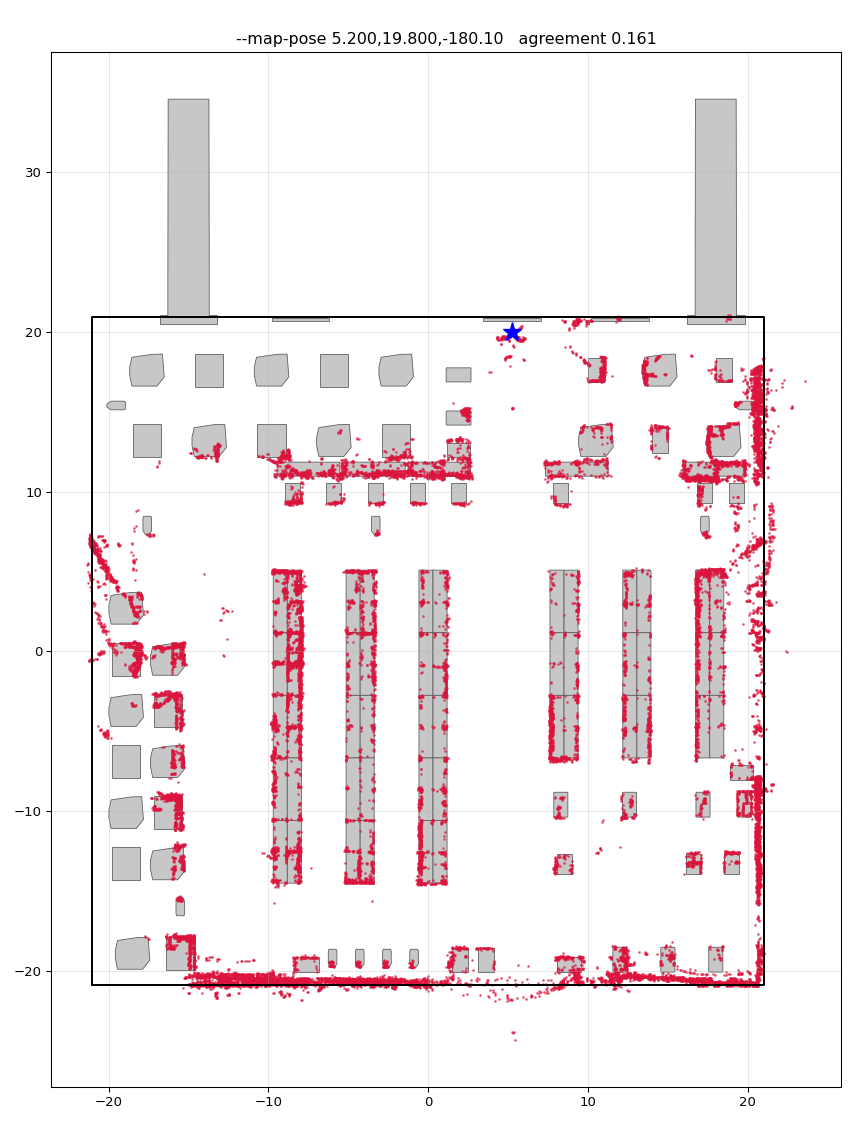
\includegraphics[width=0.7\textwidth]{figures/dataset_allsensor_realistic_map_fit.png}
  \caption[Placement overlay of the U-Bember database.]{Placement overlay of
  \repo{map/dataset_allsensor_realistic_map} (U-B). The unconstrained sweep
  preferred the \SI{180}{\degree}-rotated rival at $(-5.6, -19.6)$, agreement
  0.168 against 0.161, which puts shelf rows between shelves; the basin
  placement shown sits \SI{0.15}{\metre} from the spawn of the IMU body, as its
  build-A sibling does.}
  \label{fig:map-realistic-nov-fit}
\end{figure}

\begin{figure}[p]
  \centering
  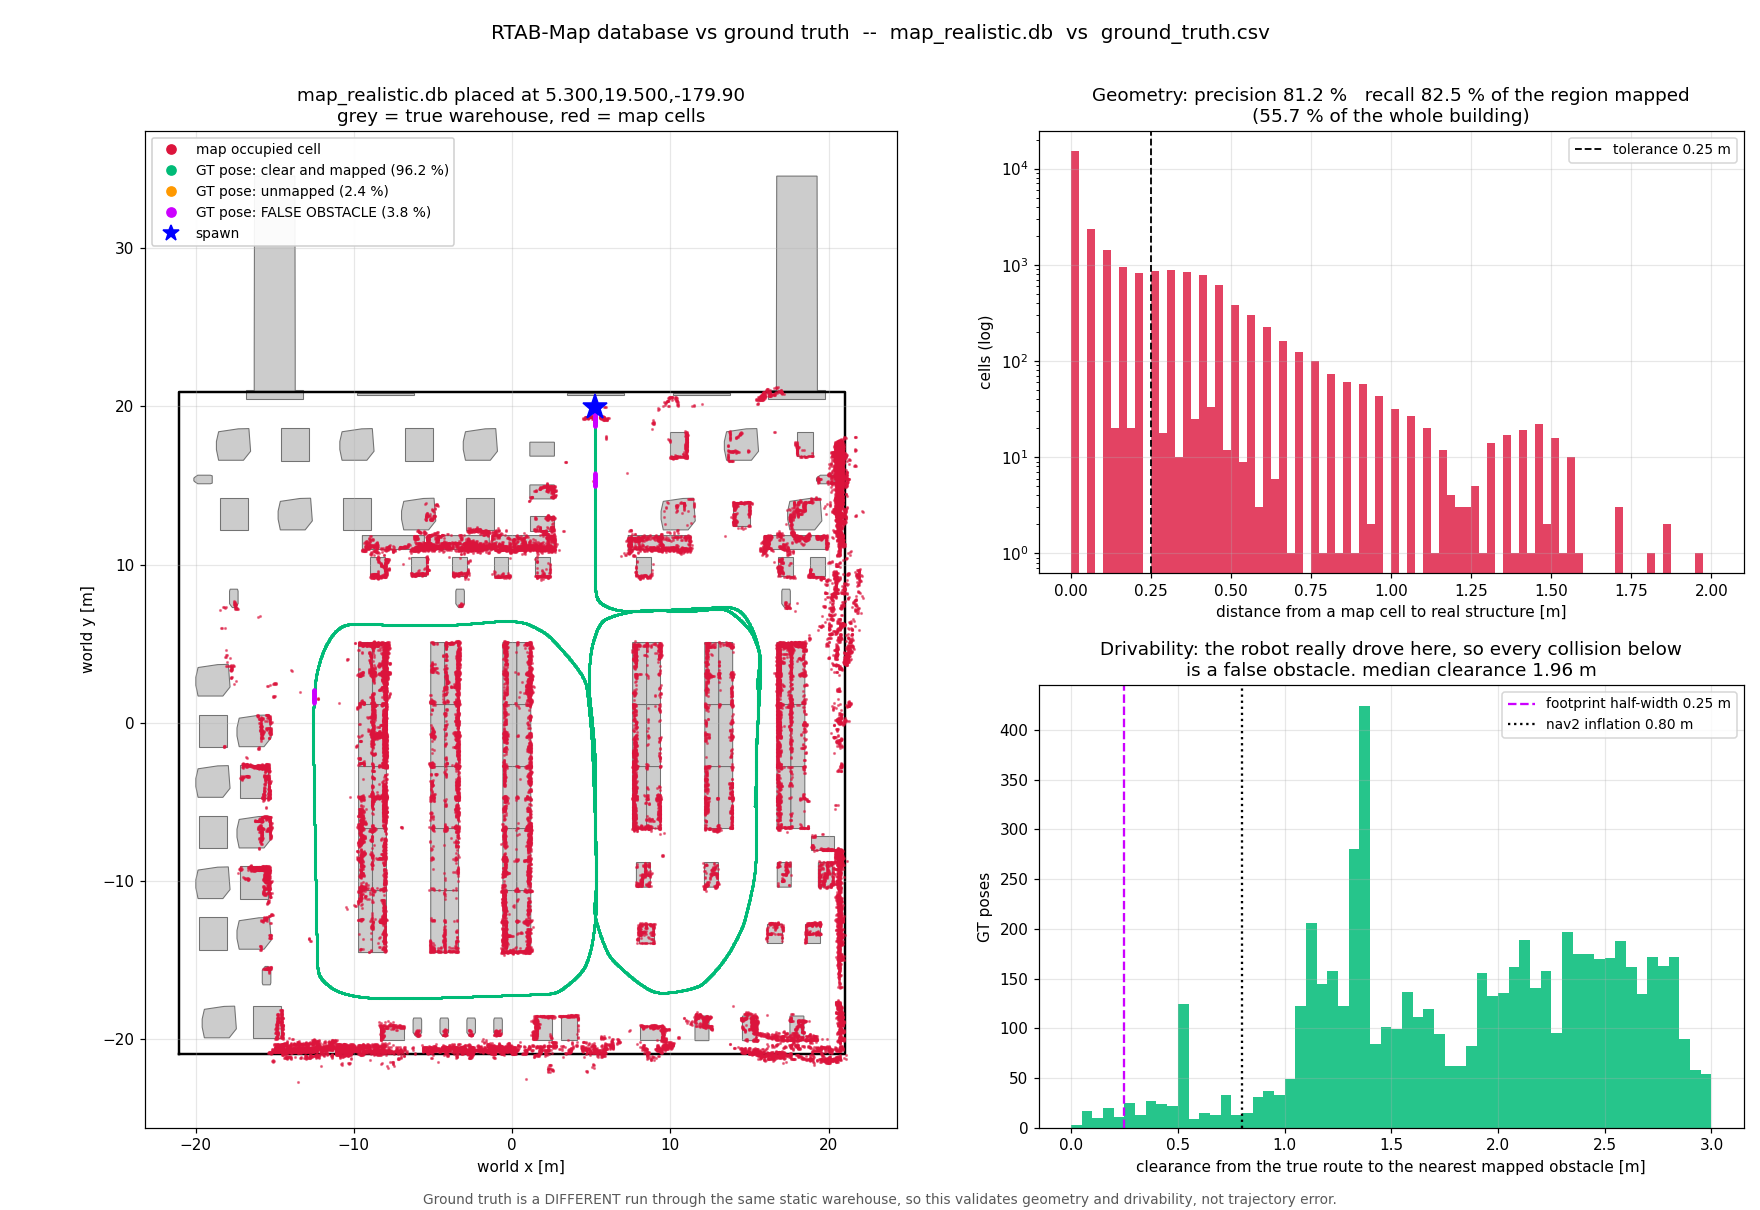
\includegraphics[width=\textwidth]{figures/map_realistic_validate.png}
  \caption[Dense-map evaluation of \repo{map/map_realistic} (U-A) against
  the independent probe.]{Dense-map evaluation of \repo{map/map_realistic}
  (U-A) against \repo{dataset_allsensor_realistic_000}. Panels as in
  \cref{fig:map-vs-gt}. The shelf rows are thickened toward the aisles; the
  false-obstacle poses sit on the first metres below the spawn and where the
  probe hugs the left shelf column at $x\approx-12.5$.}
  \label{fig:map-realistic-validate}
\end{figure}

\begin{figure}[p]
  \centering
  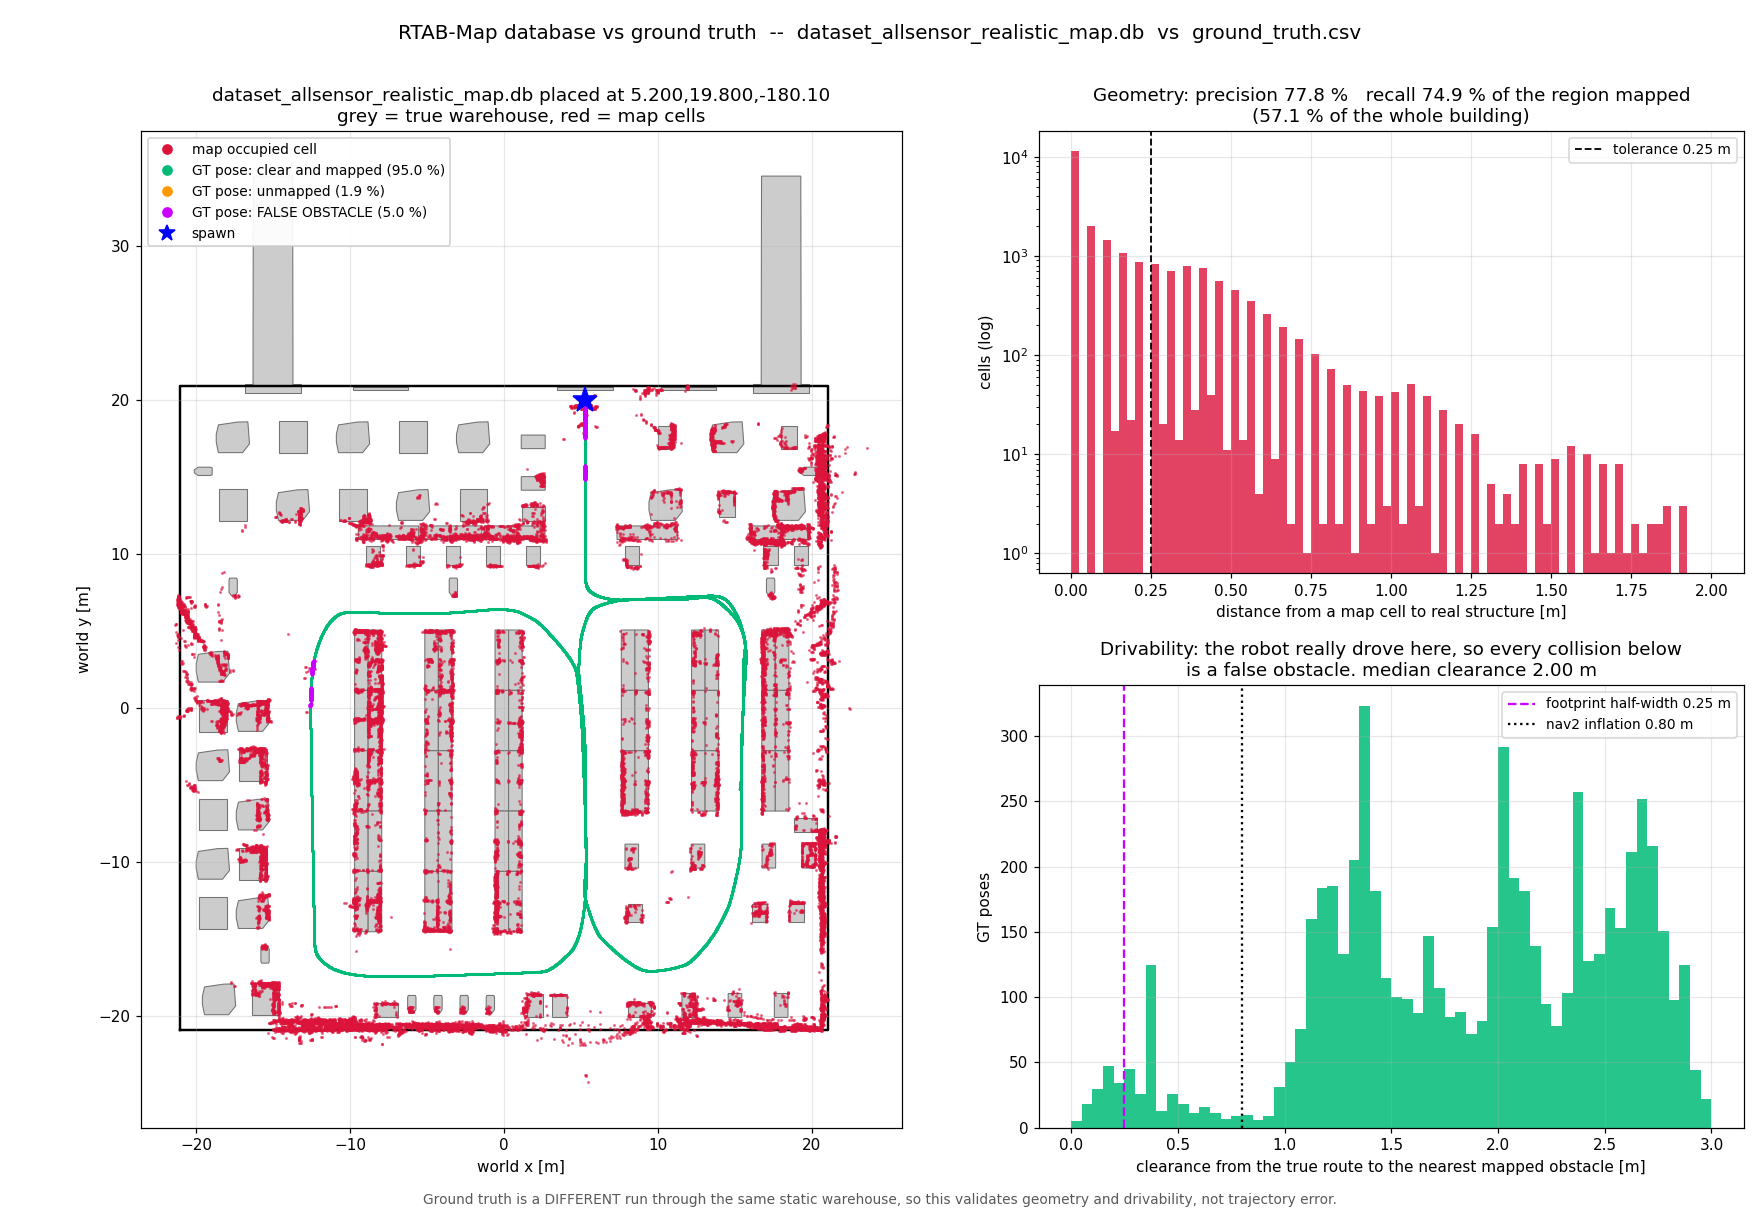
\includegraphics[width=\textwidth]{figures/dataset_allsensor_realistic_map_validate.png}
  \caption[Dense-map evaluation of the U-Bember database.]{Dense-map evaluation of
  \repo{map/dataset_allsensor_realistic_map} (U-B) against the same probe.
  The same two blocked places as U-A, the spawn stretch now longer, and more
  scatter in the outer bays and along the west wall, which this build's
  \SI{10}{\metre} grid range reaches and the build A's did not.}
  \label{fig:map-realistic-nov-validate}
\end{figure}

\begin{figure}[p]
  \centering
  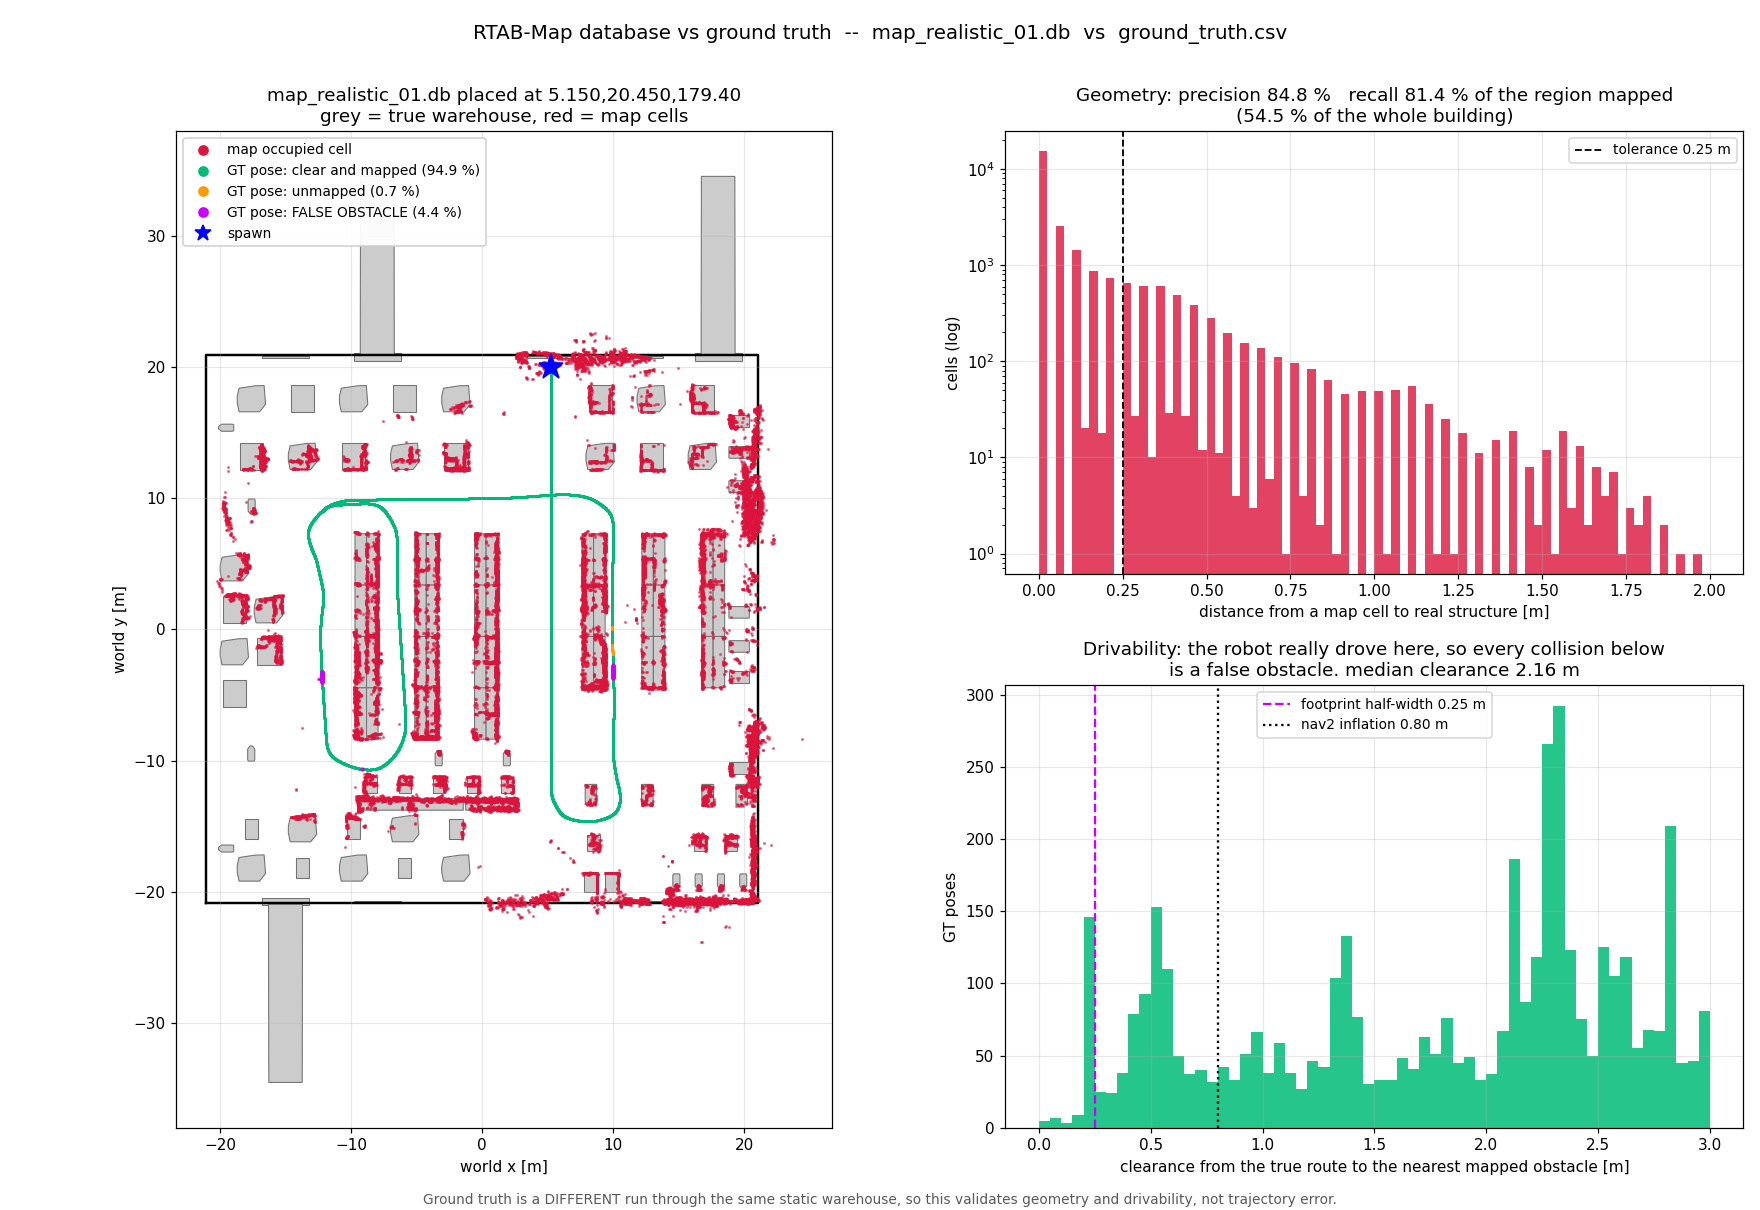
\includegraphics[width=\textwidth]{figures/map_realistic_01_validate.png}
  \caption[Dense-map evaluation of \repo{map/map_realistic_01} (I-A) against
  the independent probe.]{Dense-map evaluation of \repo{map/map_realistic_01}
  (I-A) against \repo{dataset_allsensor_realistic_001}. The clearance mode at
  exactly \SI{0.25}{\metre} is the probe threading the one-aisle gap at
  $x\approx10$ between two mapped shelf rows.}
  \label{fig:map-realistic-01-validate}
\end{figure}

\begin{figure}[p]
  \centering
  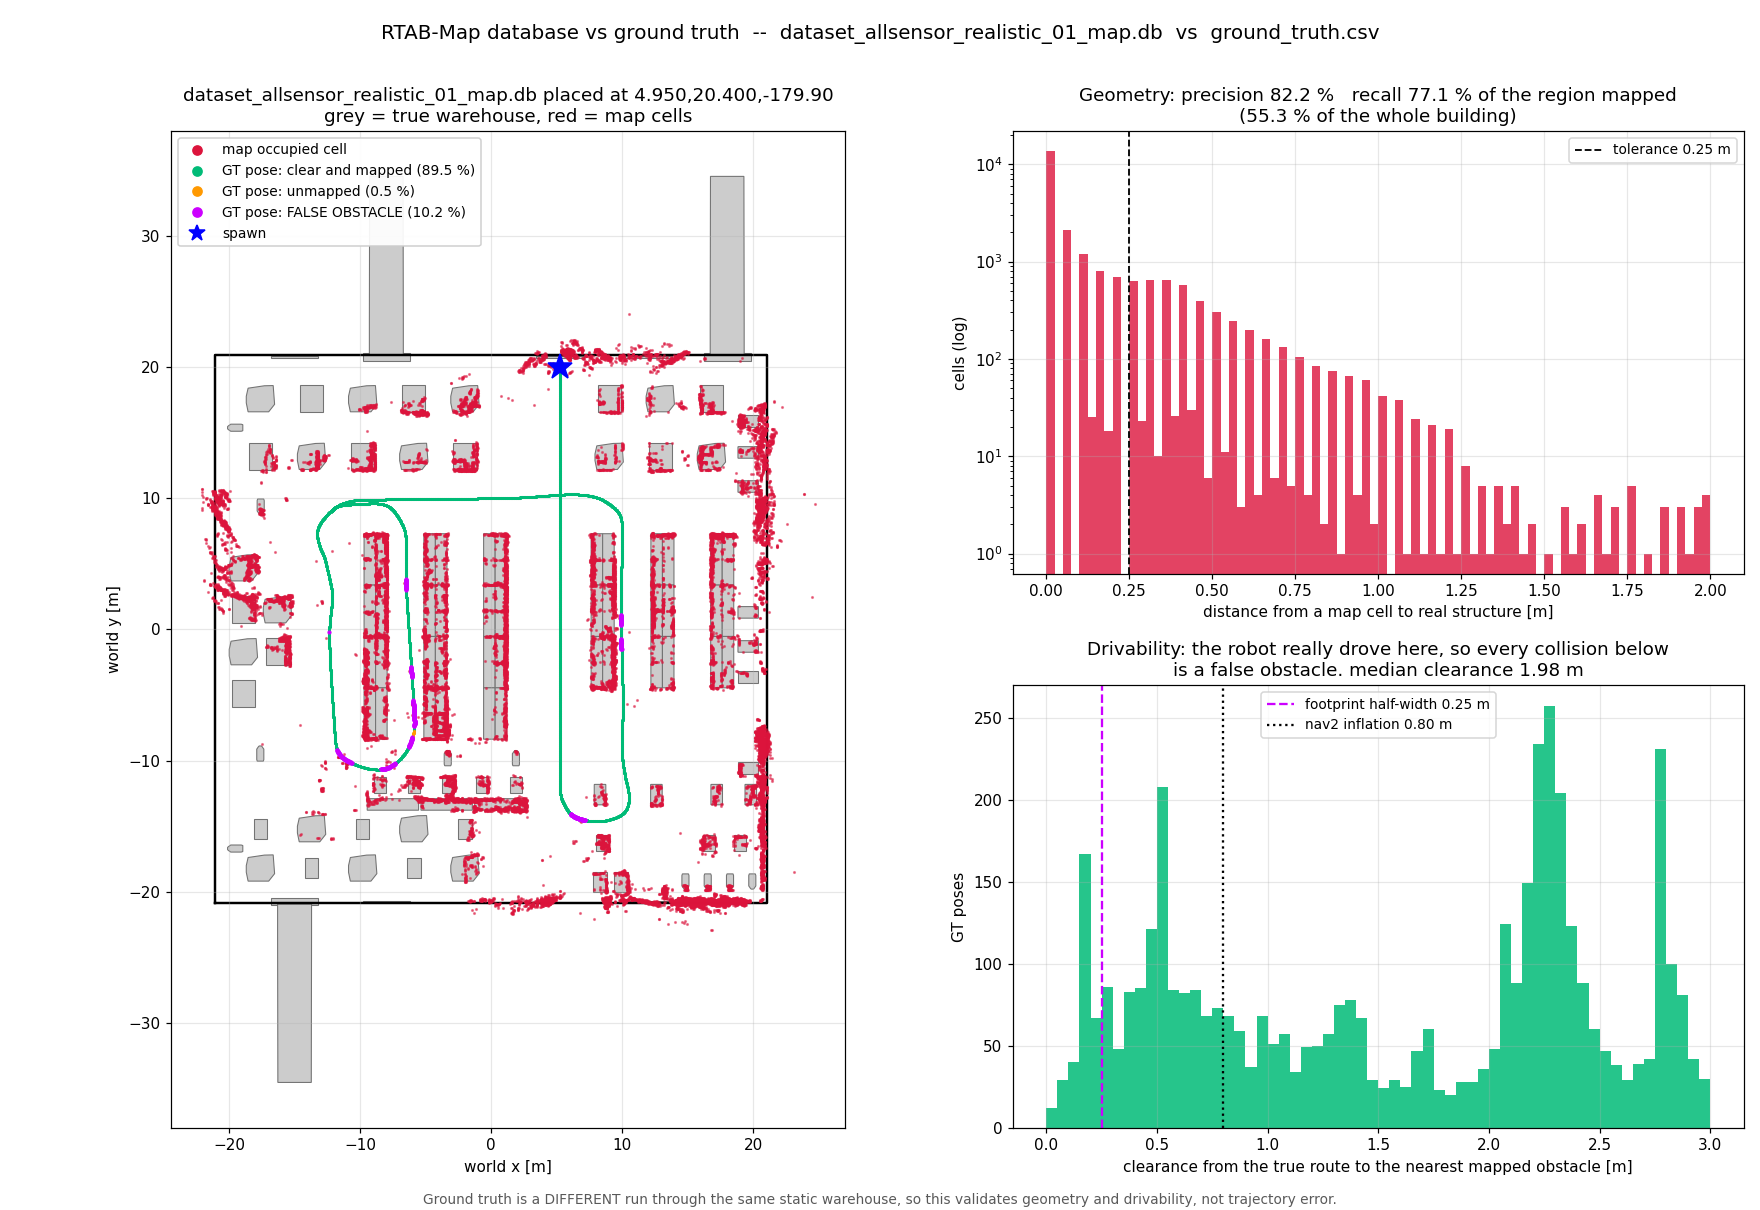
\includegraphics[width=\textwidth]{figures/dataset_allsensor_realistic_01_map_validate.png}
  \caption[Dense-map evaluation of the I-Bember database.]{Dense-map evaluation of
  \repo{map/dataset_allsensor_realistic_01_map} (I-B) against the same probe.
  The blocked poses are no longer confined to the spawn: stretches of 68, 55
  and 50 poses sit mid-route in the aisles of the probe's left loop and along
  its bottom straight, on cells the map places on the floor of the aisle.}
  \label{fig:map-realistic-01-nov-validate}
\end{figure}

\textbf{Analysis.} All four maps fail, and the build B of each recording
scores below its build-A sibling on every criterion: precision by 3.4 and 2.6
points, observed recall by 7.6 and 4.3, false obstacles from 3.8 to 5.0 and
from 4.4 to \SI{10.2}{\percent}. The build-A pair fail by similar margins on
both layouts, which made their failure a property of the build rather than of
one run; the build-B pair move it further in the same direction.

Three parameters moved together between the builds, and each has its own
signature in the data, so the reading is consistent-with, not attribution. The
detection rate, 4 to \SI{1}{\hertz}, shows as fewer nodes (148 against 165, 127
against 185) and fewer observations per cell, which the view-count effect of
the tiny-map insight analysis turns into lower precision and recall. The grid
range, 8 to \SI{10}{\metre}, shows as structure the build As never
reached: the west wall and the far outer bays now carry occupied cells, and the
largest new phantom clusters sit on them. The ground-height threshold, 0.29 to
\SI{0.10}{\metre}, shows where it would: on the I layout the build B
blocks 518 probe poses against 213, and the new stretches are mid-route, in
the aisles, on cells first observed at median node 27 rather than at the
start. A one-parameter rebuild is the test that would separate the three, and
is the next action.

In the build As the loss is mostly thickened structure, with a phantom
share the tiny map did not have. Classifying the wrong cells
(\repo{script/exp4_insights.py}): 13.4 and \SI{9.7}{\percent} of occupied
cells are surfaces drawn too thick, within \SI{0.50}{\metre} of true
structure, and 5.2 and \SI{5.3}{\percent} are phantoms further out, against
3.0 and \SI{0.4}{\percent} on the tiny map; in the build Bs the shares
are 15.4 and \SI{11.5}{\percent} thickened and 7.3 and \SI{6.3}{\percent}
phantom. The thickening sits on the shelf rows the build route passed; the
phantoms are the east and south walls, drawn about \SI{0.5}{\metre} off their
true line in all four maps and far from any route. In the build As the
false obstacles are not the thickened shelving: every blocked probe pose lies
within \SI{0.6}{\metre} of a phantom cell, the largest blocked stretch of each
map is the first metres from the spawn, and 96 and \SI{63}{\percent} of the
phantom cells under those stretches were first observed by one of the first
five graph nodes, during the inertial initialisation transient. The November U
build repeats that pattern (224 spawn poses, \SI{88}{\percent} of the blocking
cells early); the November I build does not, which is the ground-height
signature above.

All four are an odometry picture by design, and should be read as one. Loop
closure was disabled on both sides of the pipeline after the A/B of 26 October
showed the front end's own closures corrupting an otherwise \SI{0.1}{\metre}
map (RTAB-Map record \S7c), so no node was ever corrected against a revisited
place; the stored graphs confirm it, with no closure spanning more than three
nodes and none at all in the build Bs. The thickening and the displaced
walls are therefore uncorrected drift along a 365--385-metre build route
re-observing the same structure from slightly different estimated places,
which is what this configuration was built to expose. It is not evidence
about RTAB-Map's loop closing, which was not exercised.

Whole-building recall of 54.5 to \SI{57.1}{\percent} is route coverage, as on
the tiny map: the build routes loop the central block and the outer bays were
seen only in passing. Observed-region recall, the mapping figure, is 74.9 to
\SI{82.5}{\percent}.

Placement needed the overlay on three of the four fits, and the spawn check
did not apply to any. The fits land about \SI{180}{\degree} from the
\SI{-90}{\degree} spawn prediction because the map frame was seated during the
inertial initialisation transient rather than at the body's spawn pose: node 1
of the October databases carries a yaw of \SI{57}{} and \SI{-89}{\degree} and a
height still settling over the first nodes, where the tiny map's node 1 is the
identity. On the November U build the unconstrained sweep chose the rotated
rival outright; the overlays leave no doubt about any of the four placements,
and the two builds of each layout agree to \SI{0.3}{\metre} and
\SI{0.5}{\degree}.

\textbf{Limitations, each stated once.} \emph{Not route-matched:} the tiny
probe was one loop of a wide aisle, these probes thread shelf aisles
(5th-percentile clearance 0.18--0.62 against \SI{0.45}{\metre}), so part of the
false-obstacle gap is probe difficulty and the \SI{1}{\percent} threshold was
set against an easier route. \emph{No attribution:} world and route vary
together between layouts, and three parameters and the front-end session vary
together between builds, so no factor may be credited for any difference in
this slot. \emph{$n$:} one database per cell supports no uncertainty estimate.
\emph{Front end unrecorded:} the databases store the back end's parameters but
not which front end, in which session, supplied the odometry chain.

\begin{queried}[Queried: front end of the realistic builds]
RTAB-Map took its pose from TF, so the odometry came from whichever front end
was running; none of the four databases records which, and the build Bs
were made during the latency sessions of Experiment~3, whose load on the front
end is not recorded either. The precision loss cannot be placed on the front
end against the back end, nor the November drop on parameters against session,
until the build manifest names both.
\end{queried}

\paragraph{Were the poses the problem?} All four maps fail, and the failure
could lie in the trajectory the grid was built along or in how the grid was
built along it. The databases do not record which front end supplied their
odometry, so the failure cannot be placed on a front end; the poses
themselves can still be measured,
because the graph is in the database and both mapping recordings have ground
truth. \Cref{tab:map-graph-accuracy} scores every node against the recording
it was built from.

The poses are not the problem. Through the same fitted placement the occupancy
grid was scored with, the graphs sit \SI{0.102}{} and
\SI{0.128}{\metre} rms from the truth on the U layout and \SI{0.396}{} and
\SI{0.331}{\metre} on the I layout, which is \SIrange{0.03}{0.10}{\percent}
of the \SIrange{365}{381}{\metre} routes, every node of all four graphs
scored. A best-fit alignment of each graph
improves it by at most \SI{0.012}{\metre}, so the placements are right as
well: these maps are neither in the wrong place nor the wrong shape. Every one
of those figures is inside the \SI{0.25}{\metre} tolerance at which the
occupancy grids were scored, so a grid built from perfect poses would have been
scored the same way.

What follows is an attribution the chapter could not make before. The
\SIrange{77.8}{84.8}{\percent} occupied-cell precision and the
\SIrange{3.8}{10.2}{\percent} false-obstacle rate are not inherited from the
trajectory; they are produced where the grid is built from the depth image ---
the sensor range, the ground-height threshold and the ray tracing of
\cref{sec:map-eval-method} --- and that is where a fix has to be looked for.
Two qualifications hold it in place. The I-layout graphs reach
\SI{3.207}{} and \SI{2.586}{\metre} at their worst single node against
\SI{0.412}{} and \SI{0.287}{\metre} on the U layout, so the I builds do carry
a local excursion that the rms hides and that could account for part of one
layout's loss, though not for a failure both layouts share. And a graph is
scored at its nodes, one every few metres, while the grid is written from every
frame between them; a pose error that appears and is corrected between two
nodes would not be seen here.

% Generated by script/eval_map_graph.py -- do not edit by hand.
\begin{table}[htbp]
\centering
\caption[Pose accuracy of the graph each realistic map was built from.]{Pose accuracy of the graph each realistic map was built from, scored against the mapping recording's ground truth at every node stamp. ``Placed'' is the error where the map actually stands, through the fitted placement the occupancy grid was scored with, so it carries any placement error; ``aligned'' is the residual after a best-fit rigid $SE(2)$ transform of the graph itself, which absorbs placement and leaves the shape of the trajectory. Node poses are whatever TF frame the mapping session published, so each graph is scored against ground truth both at the model origin and at the IMU point and the better fit is reported. The IMU point fits better on all four, by \SIrange{0.08}{0.27}{\metre}, so the graph is closer to the estimator's frame than to the model origin; the model-origin figures would be that much larger and change no conclusion here.}
\label{tab:map-graph-accuracy}
\small
\resizebox{\textwidth}{!}{%
\begin{tabular}{llr rr rr r}
\toprule
Database & Layout & Nodes & Placed rms [\si{\metre}] & Placed max [\si{\metre}] & Aligned rms [\si{\metre}] & Aligned max [\si{\metre}] & Aligned/path [\si{\percent}] \\
\midrule
\repo{map_realistic} & U & 165 & 0.102 & 0.412 & 0.095 & 0.394 & 0.03 \\
\repo{dataset_allsensor_realistic_map} & U & 148 & 0.128 & 0.287 & 0.121 & 0.309 & 0.03 \\
\repo{map_realistic_01} & I & 185 & 0.396 & 3.207 & 0.387 & 3.102 & 0.10 \\
\repo{dataset_allsensor_realistic_01_map} & I & 127 & 0.331 & 2.586 & 0.319 & 2.464 & 0.09 \\
\bottomrule
\end{tabular}}
\end{table}


\paragraph{Summary.} Where tracking holds, the mapping pipeline is
geometrically sound on the tiny map: occupied-cell precision \SI{96.6}{\percent}
and observed-surface recall \SI{89.5}{\percent}, with whole-building recall of
\SI{67.2}{\percent} explained by route coverage; the drivability half is a dated
measurement whose independent reference is lost. On the realistic warehouse
four maps built without loop closure, two per layout under back-end
configurations A and B, are auditable end to end and all fail the same
criterion: precision 77.8 to \SI{84.8}{\percent} and false obstacles 3.8 to
\SI{10.2}{\percent} against independent probes. Their loss is thickened
shelving, displaced walls and phantoms at the spawn from uncorrected drift,
which the closure-free build was configured to expose; the current
configuration scores lower on every metric, for reasons the three parameters
it changed at once do not let this slot separate. The earlier large-warehouse
attempt that lost tracking remains unauditable.

\paragraph{Future plan.} Attribute the November drop by rebuilding one
recording with a single parameter restored at a time, first the ground-height
threshold (\repo{Grid/MaxGroundHeight}), then the detection rate, and rescoring
with the unchanged evaluator. Name the front end, its
session and the three parameters in every build manifest. Use the four maps as
the odometry baseline against which a corrected map is compared: re-enable
closure with a translation bound on accepted corrections, or merge the
closure-free sub-maps through Atlas, and rescore. Discard the cells of the
first few nodes, or start the map after the inertial transient has settled,
which the data predict would remove the spawn stretch. Record the
tiny-warehouse independent route again and retain it.

\FloatBarrier
\subsection{Real robot}
\label{sec:exp4-real}

\slotstatus{planned}{No RTAB-Map database has been built from real imagery, and
no reference geometry of the site exists to score one against.}

\textbf{Reason.} The geometry metric of \cref{sec:map-eval-method} scores
occupied cells against known collision geometry; the real site has no such
model yet, and the placement step needs it. The drivability metric needs the
motion-capture route. Neither input exists at the cutoff.

\textbf{Next action.} Survey the mock warehouse (walls, stacks, walkway) into a
reference occupancy grid at the same \SI{0.05}{\metre} resolution, build a
database from a real mapping run, and then score it with the unchanged
evaluator, using a motion-capture route from a second run for drivability.

% =====================================================================
\FloatBarrier
\section{Experiment 4: Autonomous Navigation on the Reconstructed Map}
\label{sec:exp4}

\FloatBarrier
\subsection{Simulation}
\label{sec:exp4-sim}

\slotstatus{partial}{Seven live runs on 12 November 2026, in three of the four
worlds, measure the localisation against ground truth over hand-driven routes
of \SIrange{21}{153}{\metre}. No goal was commanded in any of them, so the
goal-reaching measures of the reporting rules below are still unused and that
half of the experiment remains \status{planned}. The protocol, goal set and
success criteria are now fixed in code (\repo{script/exp4_protocol.yaml},
generated by \repo{script/exp4_goals.py}), which is what the previous revision
of this document recorded as missing.}

\textbf{Objective.} Establish whether the map of \cref{sec:exp3} is good enough to navigate on: whether the robot can relocalise
against a prior it did not build, hold that pose while driving, plan a path
through the map, and reach a sequence of goals without colliding with structure
the map got wrong. Experiment~3 scores the map as geometry; this experiment
scores it as something a planner consumes. The two are not the same question,
and the false obstacles Experiment~3 reports are the reason: a map can be
\SI{80}{\percent} precise and still block the one aisle the robot needs.

\textbf{Process.} \repo{vslam_navigation} exposes the three stages as
separate entry points, so the experiment follows them in order:
\texttt{mapping\_sim} builds the prior, \texttt{localize\_sim} gives a
read-only fix against it, and \texttt{navigate\_sim} adds the planner, the
localisation gate and the command interface. The prior is one of the databases
already scored in the simulation slot of Experiment~3, so that map quality and
navigation outcome are measured on the same artefact. The runs reported here
were driven by the operator rather than by the planner; \repo{exp4\_navigate.py}
provides both modes (\texttt{--drive} and \texttt{--run}) and records the same
data either way.

\textbf{Datasets and configuration.} The two realistic worlds of the
methodology chapter and the closure-free priors built from their mapping
recordings: \repo{dataset_allsensor_realistic_map} (U, 148 nodes) and
\repo{dataset_allsensor_realistic_01_map} (I, 127 nodes). No bag is replayed:
the simulator is driven live, because a navigation outcome depends on the
control loop and cannot be reconstructed from a recording. Every run used the
configuration frozen in the protocol file: \repo{Vis/EstimationType}~0, which
requires matched feature positions to agree in metres rather than merely to
reproject, and a \SI{5}{\second} hold on the back end so that no correction can
be latched from the front end's unstable first second. Both settings come from
the acceptance sweep of 11--12 November and are recorded in each run's
\repo{outcome.json}.

\textbf{Frames.} Ground truth is the Gazebo world frame; the prior, the
goals and the published pose are the map frame. The two are reconciled by a
closed-form planar fit of every graph node against the mapping run's ground
truth, which gives \SI{179.95}{\degree} and \SI{-179.61}{\degree} of rotation
for the U and I priors --- the map frame is the spawn, turned around --- with
median residuals of \SI{0.103}{\metre} and \SI{0.055}{\metre}. The ground truth
reports the model origin and every estimate reports the camera/IMU body, so the
\SI{0.338}{\metre} lever arm is applied to the ground truth before the fit and
before any comparison, and never to recorded data.
\flag{An earlier revision fitted against the uncorrected ground truth and
reported the resulting \SI{0.337}{\metre} residual as confirmation that the fit
was right, on the grounds that it equalled the lever arm. That was the bias, not
the evidence: a rigid transform cannot absorb an offset that rotates with the
body, so it absorbed part of it as translation and left the rest as residual.}

\textbf{Reporting rules, goal-reaching.} \flag{Fixed before any run exists,
so that the result cannot be chosen after the fact, and left unchanged here.} A
goal counts as reached when the base frame is within \SI{0.25}{\metre} and
\SI{10}{\degree} of it and the planner reports success. Per run the measures
are: the share of goals reached, the path length against the shortest
collision-free path in the ground-truth occupancy grid, the number of
collisions with true structure, the number of Nav2 recovery behaviours
triggered, the share of the run with a valid localisation fix, and the wall
time to complete the goal set. A run that loses localisation and does not
recover within \SI{30}{\second} is reported as failed, not excluded.

\textbf{Reporting rules, pose tracking.} \flag{Defined after these data
existed, and reported as the weaker claim it is.} Error is the planar distance
between the published \texttt{map}~$\rightarrow$~\texttt{base\_link} transform,
sampled at \SI{2}{\hertz}, and the lever-arm-corrected ground truth
interpolated to the same instants. That transform is used rather than
\texttt{/localization\_pose} because it is what RViz draws and Nav2 consumes,
and it includes the front end's dead reckoning between accepted fixes. The
error is reported as a median, a 95th percentile, a maximum, the median over
each half of the run, and split into the length of the mean error vector
(offset) and the standard deviation about it (scatter). A pose step over
\SI{1}{\metre} between consecutive samples is counted as a jump, excluding the
seed transition and the acquisition snap. Every run is reported on its own, as
in the other slots.

\textbf{Results.} \Cref{tab:exp4-tracking} gives the seven runs. The pose
tracks ground truth to a median of \SIrange{0.36}{0.62}{\metre}, with a median
across runs of \SI{0.499}{\metre}, and the error is bounded rather than growing:
in six of the seven runs the median over the first and second half of the run
agree. Minimum ground-truth clearance to a static model never fell below
\SI{0.58}{\metre}, so no run collided.

\begin{table}[htbp]
\centering\small
\caption{Pose tracking against ground truth, 12 November 2026. Route shapes
were driven by hand: straight, approximately square, approximately a
figure-of-eight. Offset is the length of the mean error vector, scatter the
spread about it, both over samples within \SI{2}{\metre} so that one diverged
run does not swamp them. Blind is the share of localisation poses carrying
RTAB-Map's no-information covariance.}
\label{tab:exp4-tracking}
\begin{tabular}{llrrrrrlrrr}
\toprule
World & Route & Driven & Dur. & Med. & p95 & Max & 1st/2nd & Offset & Scatter & Blind \\
      &       & (m)    & (s)  & (m)  & (m) & (m) & half (m) & (m) & (m) & \\
\midrule
U static  & straight & 24.7  & 25  & 0.499 & 0.562 & 0.58  & 0.50/0.45 & 0.466 & 0.057 & 0.045 \\
U static  & square   & 109.6 & 86  & 0.509 & 6.153 & 6.71  & 0.42/5.94 & 0.299 & 0.111 & 0.016 \\
U static  & figure-8 & 153.0 & 124 & 0.404 & 4.017 & 4.13  & 0.46/0.38 & 0.019 & 0.086 & 0.013 \\
I static  & straight & 20.9  & 25  & 0.359 & 0.530 & 0.55  & 0.43/0.34 & 0.322 & 0.150 & 0.158 \\
I static  & square   & 67.2  & 57  & 0.517 & 0.759 & 0.97  & 0.48/0.57 & 0.143 & 0.153 & 0.068 \\
I static  & figure-8 & 124.5 & 122 & 0.438 & 0.757 & 16.77 & 0.42/0.46 & 0.138 & 0.120 & 0.047 \\
U dynamic & straight & 26.0  & 30  & 0.624 & 1.275 & 1.35  & 0.62/0.55 & 0.588 & 0.247 & 0.103 \\
\bottomrule
\end{tabular}
\end{table}

\FloatBarrier
\paragraph{Insight: the error is the map's displacement, measured from the other
side.} The error is dominated by a constant offset, not by scatter: scatter is
\SIrange{0.06}{0.25}{\metre} across the seven runs while the offset reaches
\SI{0.59}{\metre}. The offset is also route-dependent in a way that identifies
its source. The three straight single-aisle drives carry
\SIrange{0.32}{0.59}{\metre}; the two routes that cover the building average to
\SI{0.019}{\metre} and \SI{0.138}{\metre}. A pose pulled onto a map whose local
geometry is displaced inherits that displacement while it stays in one region,
and averages it away over a route that visits many.

Experiment~3 measured the same quantity directly and independently: on all four
realistic maps the walls are displaced about \SI{0.5}{\metre} as phantom bands,
and the shelf fronts are drawn \SIrange{9.7}{15.4}{\percent} too thick. The two
figures agree in magnitude, from a cell-by-cell comparison of the grid against
the world in one case and from a pose comparison against ground truth in the
other. The reading is that this slot's accuracy is \emph{map-limited rather than
estimator-limited}: the estimator's own jitter is under a quarter of a metre,
and what remains is the prior being locally wrong. It also predicts the
improvement to chase --- a better map, not a better filter --- and it is
consistent with Experiment~3's recall result, that surfaces seen edge-on and
once are the ones reproduced worst, since a straight aisle drive sees its
surfaces grazing.

\paragraph{Insight: the initialisation transient damages both layers.}
Experiment~3 attributes the blocking false obstacles of three of the four
realistic maps to phantom cells laid by the first five graph nodes
(\SIrange{63}{96}{\percent} of them), and names discarding those cells, or
starting the map after the inertial transient has settled, as the one
correction its data predict would help. The same transient was found
independently in this slot, one layer up: the front end's orientation is
unstable for about a second after it starts, and a back end that accepts a fix
during that window latches a correction \SIrange{73}{76}{\degree} wrong and
holds it for roughly \SI{16}{\second}. Holding the back end back for
\SI{5}{\second} removed it, confirmed over three runs by the collapse of the
largest correction yaw from \SIrange{110}{177}{\degree} to \SI{25}{\degree}.
Neither \repo{wait_for_imu_init} nor the pose gate's \repo{init_ignore_s}
prevents it: the first tests inertial validity, which is already true through
the unstable window, and the second only withholds the pose from Nav2 after the
correction has been formed. One transient, two symptoms, and the same
prescription in both places --- do not consume the first second.

\textbf{Failures.} One run of the seven lost the pose. The U static square
route tracked at \SI{0.42}{\metre} through its first half and
\SI{5.94}{\metre} through its second, with four jumps, and did not recover
before the run ended. It is reported, not excluded. A second run, the I static
figure-of-eight, shows a \SI{16.77}{\metre} maximum against a 95th percentile
of \SI{0.76}{\metre} and flat halves: a single transient that recovered, which
the maximum alone would not distinguish from the failure above.

Availability is the weaker column. The I static straight run carried no
information for \SI{15.8}{\percent} of its poses and the U dynamic run for
\SI{10.3}{\percent}, against a criterion of \SI{10}{\percent}. Accuracy in both
was ordinary when a fix existed, so the difficulty is holding the fix rather
than obtaining one.

\textbf{Traffic.} The one dynamic run is the worst of the seven on both
offset (\SI{0.588}{\metre}) and scatter (\SI{0.247}{\metre}, about double the
static runs) and sat unlocalised \SI{10.3}{\percent} of the time. One run
decides nothing, but it points the same way as Experiment~1's finding that
traffic degrades the estimate without breaking tracking.

\textbf{What these data cannot answer.} Every cell is a single run, and the
acceptance sweep of 11--12 November established that this stack's run-to-run
spread over identical settings is as wide as most differences between settings,
so no comparison between worlds, layouts or routes in
\cref{tab:exp4-tracking} is evidence. The routes were driven by hand and
differ in shape and length, so route is a confound rather than a factor. No
goal was commanded, so nothing here speaks to planning, to the false-obstacle
question that motivates the experiment, or to recovery behaviour. One dynamic
world is sampled and one is not.

\textbf{Next action.} Collect the dynamic worlds and reps 2 and 3 of every
cell, then run the goal set with \texttt{--run} so the goal-reaching rules above
can be applied. The narrow question still outstanding is Experiment~3's: does
the \SIrange{3.8}{10.2}{\percent} false-obstacle rate block a route, or does the
planner drive around it.

\FloatBarrier

\FloatBarrier
\subsection{Real robot}
\label{sec:exp4-real-nav}

\slotstatus{planned}{No real-robot navigation run has been made, and the real
rig has no map to navigate on: the dense-map slot of \cref{sec:exp4-real} is
itself planned, because no RTAB-Map database has been built from real imagery
and no reference geometry of the site exists to score one against.}

\textbf{Objective.} As in simulation, on the real rig.

\textbf{Next action.} Blocked behind the real-robot half of Experiment~3: a map
must exist before navigation on it can be scored.

% =====================================================================
\FloatBarrier
\section{Cross-Experiment Discussion, Simulation-to-Real Comparison and
Limitations}
\label{sec:results-discussion}

\FloatBarrier
\subsection{Simulation against the real robot}
\label{sec:sim-vs-real}

Two slots now hold a number in both domains, and the comparison they allow is
narrow and consistent. ORB-SLAM3 with the GPU front end and no divergence
event holds \SIrange{0.14}{0.52}{\metre} aligned ATE on the realistic
simulated warehouse (\cref{sec:results-validity}) and, against the optical
tracker, \SIrange{0.25}{0.27}{\metre} on \repo{realv7_000} and
\SIrange{0.46}{0.52}{\metre} on \repo{realv6_000} (\cref{sec:exp1-real}); the
real figures are planar and provisional until the marker lever arm is
measured, and the routes are a fifth to a tenth as long, so the agreement in
metres is of order, not of value.

Normalising by distance travelled removes the route length from that
comparison and reverses its reading. As a percentage of the ground-truth path
the fifteen simulated runs that held tracking lie between \SI{0.09}{} and
\SI{0.64}{\percent} (\cref{tab:realistic-baseline}); every real run lies
above that band --- \SIrange{1.16}{1.24}{\percent} on \repo{realv7_000},
\SIrange{1.40}{4.04}{\percent} on \repo{_001} and
\SIrange{0.74}{0.85}{\percent} on \repo{_002} (\cref{tab:realv7-patch15})
--- except the four \repo{_002} runs, which fall inside it. One thing
qualifies that before it is read as a measurement of the reality gap: the
ratio penalises a short route, because a fixed start-up error is divided by
\SIrange{21}{23}{\metre} on the real robot and by up to \SI{172}{\metre} in
simulation, and no real recording long enough to remove that bias exists.
What the normalised figures do establish is the negative: per metre driven the
real and simulated results are not equivalent, and the agreement in metres
should not be read as though they were.

The two domains also differ in what the error is made of, and the difference
identifies where each one comes from. In simulation the visual error is scatter
about the truth: the mean of each signed component is
\numrange{0.17}{0.36} of its RMS in every arm
(\cref{tab:exp1-translation-pattern}). In navigation against a prior map it is
the opposite, a constant offset that reaches \SI{0.59}{\metre} against scatter
of \SIrange{0.06}{0.25}{\metre} (\cref{tab:exp4-tracking}). The two are
consistent once the references are separated: \cref{sec:exp1-sim} scores
against ground truth directly and sees only the estimator's own jitter, while
\cref{sec:exp4-sim} scores a pose pulled onto a map that is itself displaced.
The reading is that the offset belongs to the map and the scatter to the
estimator, which is the same conclusion \cref{sec:exp4-sim} reaches from its
own data and by a different route.

Its failure modes differ by domain. In simulation every divergence is
the loop closer's: a false closure between the repeated aisles of the I layout
in both front ends, and a vertical drift that only the closer corrects. On the
real robot the closer changed nothing on either recording set, and the
failures were the inertial initialisation (an upstream map reset at the
initialisation and a starved re-initialisation on nine \repo{realv7} runs) and
the CPU front end's frame loss at real time. VINS-Fusion has the opposite
record: the most accurate estimator on every simulated recording
(\SIrange{0.22}{0.66}{\metre}, no jump) and no valid real run on any of the
four, through IMU delivery and configuration defects that are diagnosed and
in part corrected but not yet re-run. The non-visual baseline now exists in both
domains. In simulation the measured-noise filter is the more accurate of the
two families; on the real robot wheel+gyro dead reckoning with one fitted
speed scale holds \SIrange{0.22}{0.46}{\metre} on the held recordings
against the best visual run's \SIrange{0.17}{0.46}{\metre}
(\cref{sec:exp1-real}), leading on one, tying on one and losing the third to
the patch-15 re-runs of \repo{realv7_002}. The claim the chapter can carry is
therefore that the two are in the same accuracy class on routes of this
length, not that either family wins; and the two hypotheses the project is named for,
filtering and dense mapping, have no real-robot number at all. What the
simulation slots establish for the real campaign is the order in which its
risks should be retired: the inertial noise model and the initialisation
before any pipeline is tuned (\cref{sec:results-proprio,sec:exp1-real}); the
loop closer's correction bound before it is trusted in repeated structure
(\cref{sec:results-validity}); and the detector's moving-object recall of 0.29, which bounds any filtering
benefit before the filter is judged (\cref{sec:yolo-performance}).

\FloatBarrier
\subsection{Limitations}
\label{sec:results-limitations}

\Cref{tab:limitations} lists the limitations of the results reported in this
chapter with the consequence each one carries. ``Scope'' identifies the
experiment affected.

\begin{table}[htbp]
\centering
\caption[Limitations of the results reported in this chapter, and what each one prevents.]{Limitations of the results reported in this chapter, and what each one
prevents. Scope: 1--4 the experiment, S simulation, R real robot.}
\label{tab:limitations}
\small
\begin{tabularx}{\textwidth}{l>{\raggedright\arraybackslash}p{0.38\textwidth}>{\raggedright\arraybackslash}X}
\toprule
Scope & Limitation & Consequence \\
\midrule
all S & one run per cell on the four accuracy recordings & no mean, deviation
  or interval there; the only repeated runs are the three per configuration on
  the two mapping recordings \\
1 S & ORB-SLAM3 repeats to \SI{0.089}{\metre} on one mapping recording and
  \SI{0.277}{\metre} on the other, against VINS-Fusion's \SI{0.035}{} to
  \SI{0.094}{\metre} (\cref{tab:mapping-repeats}) & an ORB-SLAM3 difference
  under about \SI{0.25}{\metre} is inside run-to-run spread; the divergences
  and the front-end comparison are not \\
all S & route and traffic confounded: no two recordings share a route &
  traffic is a condition of a recording, not a tested factor \\
all & one laptop, one replay rate, per-process resource figures & no evidence
  of real-time capability on the robot's computer; frame retention is a
  property of this machine \\
1 S & the shared inertial noise model was fitted to neither family & the
  EKF--VIO ordering is a tuning result; the measured-noise filter shows the
  size of the effect \\
1 S & idealised simulated encoders, slip under \SI{1}{\percent} & the
  proprioceptive estimators' best case \\
1 R & the wheel speed scale is fitted against the tracker on one recording,
  not measured; the steering feedback is a command echo & the baseline has
  one tuned constant and no yaw-rate observation, so no EKF \\
2 S & projected truth with exemptions; the walking people are actors without
  pose or mesh and outside the detector's classes & the scored basis is the
  easier one; people are unscorable and unmaskable \\
1 S & the ATE is three-dimensional & vertical drift is charged to a floor
  robot; the planar onset table is the complement \\
3, all & the path-normalised column divides by route length, and the real
  routes are a fifth to a tenth of the simulated ones & a fixed start-up error
  costs a short route more, so the simulated figures are flattered; the
  comparison bounds the gap's direction, not its size \\
1 S & the false closure is diagnosed from its correction, not its images &
  a diagnosis, not a fix \\
1 S & the mapping-recording repeats were run one configuration at a time, not
  interleaved, on a laptop that throttles & the I-recording front-end
  comparison is confounded with thermal state \\
1 R & marker-to-IMU lever arm unmeasured; \repo{realv6} tracker export at
  \SI{1.7}{\hertz} fails the validity rules & every real ATE provisional;
  \repo{realv6} values are diagnostics \\
1 R & VINS-Fusion has no valid real run & no real-robot estimator comparison \\
1 R & patch 15 is exercised on all twelve runs
  (\cref{tab:realv7-patch15}), one run each & the repair is no longer needed,
  but there is still one run per configuration, so the comparison with the
  repaired stock figures is run against run \\
1 R & the IMU noise densities were also changed between the two sets of
  \repo{realv7_002} runs, and no artefact records which the earlier set used &
  the loss of the tilt is attributable to patch 15, the size of the accuracy
  gain is not \\
3 S & the tiny map's independent drivability route is lost & its drivability
  result cannot be regenerated \\
3 S & the two configurations of each realistic map are one build each & the
  parameter attributions are signatures, not ablations \\
3 R & no real-imagery database & the slot is planned \\
\bottomrule
\end{tabularx}
\end{table}

No root cause is assigned in this chapter beyond what a run's own artefacts
show: the loop-closure corrections, the manifests, the initialisation logs. The
decisions the chapter leaves open are the ones the Open Concerns document
collects.
